\documentclass[12pt,a4paper,titlepage]{article} %twopage

%Befehle

%Grafik einbinden
%\centering
%\includegraphics[width=0.7\textwidth]{Bild.pdf}


%\usepackage{german} %deutsches Format
\usepackage[ngerman]{babel}
\usepackage[utf8]{inputenc} %Umlaute
\usepackage{graphicx} %Grafiken einbinden
\usepackage{amsmath,amssymb,amsthm}
\usepackage{nicefrac}
\usepackage{marvosym}[Lightning]
\usepackage{array}
\usepackage{dsfont} %statt \mathbb{1}
\usepackage{tikz}
\usetikzlibrary{matrix}
\usepackage{hyperref} %Hyperlinks in pdf

%Metadaten
\hypersetup{
	pdftitle = {Analysis I Skript (WS 18/19)},
	pdfauthor = {Pavel Zwerschke, Daniel Augustin}}

\theoremstyle{definition}
\newtheorem{satz}{Satz}[subsection]
\newtheorem{kor}[satz]{Korollar}
\newtheorem{lem}[satz]{Lemma}

\newtheorem{defi}[satz]{Definition}
\newtheorem*{beh}{Behauptung}

\theoremstyle{remark}
\newtheorem*{bem}{Bemerkung}
\newtheorem*{bsp}{Beispiel}

\newenvironment{bew}{\begin{proof}[Beweis]}{\end{proof}}
\newcommand{\N}{\mathbb{N}}
\newcommand{\Z}{\mathbb{Z}}
\newcommand{\Q}{\mathbb{Q}}
\newcommand{\R}{\mathbb{R}}
\newcommand{\gqq}[1]{\glqq{}#1\grqq{}}
\newcommand{\limes}[1]{\lim\limits_{#1\rightarrow\infty}}

\begin{document}
\title{Analysis I (WS 18/19)}
\date{\today}
\author{Pavel Zwerschke, Daniel Augustin}
\maketitle

%Inhaltsverzeichnis
\tableofcontents
\newpage

\setcounter{section}{-1}
\section{Organisatorisches}
\textbf{Dozent}\\
Prof. Dr. Dirk Hundertmark (20.30, 2.028)\\
\href{mailto:dirk.hundertmark@kit.edu}{dirk.hundertmark@kit.edu}\\
\textbf{Übungsleiter}\\
Dr. Markus Lange (20.30, 2.030)\\
\href{mailto:markus.lange@kit.edu}{markus.lange@kit.edu}\\
\textbf{Übungszettel}\\
Ausgabe:\\
donnerstags unter \href{http://www.math.kit.edu/iana1/lehre/ana12018w/}{\texttt{www.math.kit.edu/iana1/lehre/ana12018w/}}\\
Abgabe:\\
bis mittwochs um 19:00 in den Abgabekästen des Foyers des Mathematikgebäudes (20.30)\\
getackert, mit Namen, Matrikelnummer, Tutoriennummer und Deckblatt (optional) in das Fach mit der richtigen Kennzeichnung legen\\
Zettel dürfen zu zweit abgegeben werden\\
\textbf{Übungsschein}\\
Jede K-Aufgabe wird mit 4 Punkten bewertet. Einen Übungsschein erhält wer 50\% der Punkte aller K-Aufgaben erzielt.\\
\textbf{Klausur}\\
Die Anmeldung findet über das Online-Portal statt. Die Klausur findet am 26.03.2019 von 08:00 bis 10:00 statt. Der Übungsschein ist Voraussetzung für die Teilnahme an der Klausur.

\newpage
%17.10.2018
\section{Was ist Analysis?}
\textbf{Mathematik:} Streng logisches Herleiten neuer Aussagen (aus möglichst wenigen Grundannahmen, sog. Axiomen).\\
\textbf{Analysis:} Aus dem altgriech. \glqq Auflösen\grqq. Analysis hat ihre Grundlage in der \glqq Infinitisemalrechnung\grqq  von Leibnitz und Newton.\\
\textbf{Zentrale Begriffe:} Grenzwerte von Folgen und Reihen, Funktionen, stetig, differenzierbar, integrieren, Differential- und Integralrechnung, Differentialgleichungen (Newton, Maxwell, Schrödinger), unendlich dimensionale Räume
\begin{bsp}
	\(S = \frac{1}{2} + \frac{1}{4} + \dots + \frac{1}{2^n} + \dots\\
	2S = 1 + \frac{1}{2} + \dots + \nicefrac{1}{2} + \dots\\
	2S = 1 + S\)\\
	\(S\) entspricht der Wahrscheinlichkeit, dass irgendwann mal Kopf in einem Münzwurf kommt.\\
	Vorsicht!\\
	\(S = 1 + 2 + 4 + \dots\\
	2S = 2 + 4 + 8 + \dots = -1 + 1 + 2 + 4 + \dots = -1 + S\\
	S = -1\)\\
	Natürlich Quatsch!\\
  	Formales Rechnen kann gefährlich sein!

	\begin{itemize}
		\item Was sind mathematische Aussagen?
		\item Wie macht man Beweise, wie findet man sie? (learning by doing)
		\item logische Zusammenhänge
		\item Was sind Zahlen?
	\end{itemize}
\end{bsp}
\section{Etwas Logik}
Eine (mathematische) Aussage ist ein Ausdruck, der wahr oder falsch ist.\\
z. B.
\begin{enumerate}
  \item \(A :\) \gqq{\(1+1=2\).}  (auch \gqq{\(1+1=3\)}, \gqq{\(1+1=0\)})
  \item \(B :\) \gqq{Es gibt unendlich viele Primzahlen.}
  \item \(C :\) \gqq{Es gibt unendlich viele Primzahlen \(p\), für die \(p + 2\) auch eine Primzahl ist.} (Primzahlzwillingsvermutung)
  \item \(D :\) \gqq{Die Gleichung \(m \ddot{x} = F\) hat, gegeben \(\dot{x}(0) = v_0, x(0) = x_0\), immer genau eine Lösung.} (Lösung der Newtonschen Gleichung)
  \item \(E :\) \gqq{Jede gerade natürliche Zahl größer als 2 ist die Summe zweier Primzahlen.} (Goldbachsche Vermutung)
  \item \(F :\) \gqq{Morgen ist das Wetter schön.}
  \item \(G :\) \gqq{Ein einzelnes Atom im Vakuum mit der Kernladungszahl \(Z\) kann höchstens \(Z+1\) Elektronen binden.} (Ionisierungsvermutung, es ist noch nicht einmal bekannt, ob es eine Zahl \(Z\) gibt, sodass höchstens \(Z+1\) Elektronen gebunden werden.)
  \item \(H(k,m,n) :\) \gqq{Es gilt: \(k^2 + m^2 = n^2\).} (z. B. \(H(3,4,5)\) ist wahr.)
\end{enumerate}
Gegeben für natürliche Zahlen \(n\), Aussagen \(A(n)\), dann gilt:\\
Für jede nat. Zahl \(n\) ist \(A(n)\) wahr, genau dann, wenn 
\begin{enumerate}
  \item \(A(1)\) ist wahr.
  \item Unter der Annahme, dass \(A(n)\) wahr ist, folgt, dass \(A(n+1)\) wahr ist.
\end{enumerate}
\begin{bsp}
	\(A(n): 1+2+3+\dots+n=\frac{n(n+1)}{2}\).
\end{bsp}
\begin{bew} 
	Vollständige Induktion\\
	Induktionsanfang:\\
	$1 = \frac{1(1+1)}{2} \checkmark$\\
	Induktionsschluss:\\
	Wir nehmen an, dass $A(n)$ wahr ist (für $n\in\mathbb{N}$)\\
	D. h. Induktionsannahme:\\
	$1+2+3+\dots+n=\frac{n(n+1)}{2}$\\
	Dann folgt:\\
	$\underbrace{1+2+\dots+n}_{=\frac{n(n+1)}{2}}+(n+1)=\frac{n(n+1)}{2}+(n+1) \\
	=\frac{n(n+1) + 2(n+1)}{2} = \frac{(n+1)(n+2)}{2} = \frac{(n+1)((n+1)+1)}{2}$
\end{bew}
%18.10.2018
\begin{bem}
	Gaußscher Trick:\\
	1)\\
	$S=1+2+3+\dots+n=n+(n-1)+(n-2)+\dots+2+1\\
	2S = \underbrace{(n+1)+(n+1)+\dots+(n+1)}_{n\text{-mal}} \Leftrightarrow S = 
	\frac{n(n+1)}{2}$.\\
	2)\\
	$S_n = 0 + 1 + 2 + \dots + n\\=$ Anzahl der Punkte in\\
	%BILD EINFUEGEN
	$\approx$ Fläche eines rechtwinkligen Dreiecks $=\frac{1}{2}*n*n$.\\
	Also: Ansatz (\glqq geschicktes Raten\grqq , \glqq scientific guess\grqq , englisch: ansatz):\\
	$S_n = \underbrace{a_2 n^2 + a_1 n + a_0}_{\text{Polynom 2. Grades in n}}\\
	a_2 = \frac{1}{2}$\\
	Wie bekommt man $a_0, a_1, (a_2)$?
	$n=0: S_0 = 0 = a_2*0^2+a_1*0+a_0 \Rightarrow a_0 = 0$.\\
	$n=1: S_1 = 1 = a_2*1^2+a_1*1^2 = a_2 + a_1 = \frac{1}{2} + a_1$.\\
	also: $a_1 = \frac{1}{2}$\\
	$\Rightarrow$ Raten: $S_n = \frac{1}{2}n^2 + \frac{1}{2} n = \frac{n(n+1)}{2}$.
\end{bem}

\subsection{Grundbegriffe}
Aussagen: Notation\\
\begin{tabular}{r|l}
	$:$ & \glqq so, dass gilt\grqq\\
	$\exists$ & \glqq es gibt mindestens ein\grqq , \glqq es existiert\grqq\\
	$\forall$ & \glqq für alle\grqq\\
	$\Rightarrow$ & \glqq impliziert\grqq($A \Rightarrow B$ \glqq aus $A$ folgt $B$\grqq)\\
	$\Leftrightarrow$ & \glqq genau dann, wenn\grqq\\
	$\neg A$ & nicht $A$\\
	$A \wedge B$ & $A$ und $B$\\
	$A \vee B$ & $A$ oder $B$\\
	$A := B$ & $A$ ist per Definition gleich $B$
\end{tabular}

\begin{satz}
	Folgende Aussagen sind allein aus logischen Gründen immer wahr.
	\begin{tabular}{rl}
		$\neg(\neg A) \Leftrightarrow A$ & Gesetz der doppelten Verneinung\\
		$A \Rightarrow B \Leftrightarrow \neg B \Rightarrow \neg A$ & Kontraposition\\
		$A \Rightarrow B \Leftrightarrow (\neg (A \wedge \neg B))$ & beim Widerspruchsbeweis\\
		$\neg(A \wedge B) \Leftrightarrow (\neg A \vee \neg B)$ & de Morgan\\
		$\neg(A \vee B) \Leftrightarrow (\neg A \wedge \neg B)$ & de Morgan\\
	\end{tabular}
\end{satz}
\begin{bem}
	$A \Rightarrow B \Leftrightarrow B $ ist mindestens so wahr wie $A \Leftrightarrow A$ ist mindestens so falsch wie $B \Leftrightarrow \neg B \Rightarrow \neg A$.\\$(A\Leftrightarrow B) \Leftrightarrow (A \Rightarrow B \wedge B \Rightarrow A)$.
\end{bem}
\begin{bsp}
	$n \in \mathbb{N}$ ist gerade, falls $k \in \mathbb{N}$ existiert mit $n = 2k$.\\
	$n\in \mathbb{N}$ ist ungerade, falls $\exists k\in \mathbb{N}_0: \vee n = 2k+1$.\\
	Dann gilt: $n$ ist gerade $\Leftrightarrow n^2$ ist gerade.
	\begin{bew}
		\glqq $\Rightarrow$\grqq : $n$ gerade $\Rightarrow n=2k$, für $k\in \mathbb{N}$\\
		$n^2 = (2k)^2 = 4k^2 = 2(2k^2)$ ist gerade.\\
		Umgekehrt müssen wir zeigen:\\
		\glqq $\Leftarrow$\grqq : $n^2$ gerade $\Rightarrow n$ gerade\\
		Kontraposition: $n$ ungerade $\Rightarrow$ $n^2$ ungerade\\
		Also sei $n = 2k+1, k \in \mathbb{N}_0 \Rightarrow n^2 = (2k+1)^2 = 4k^2 + 4k + 1 = \underbrace{2(2k^2 + 2k)}_{\text{gerade}} + 1 \Rightarrow n^2$ ist ungerade. 
	\end{bew}
\end{bsp} 
\textbf{Mengen} (nach Cantor)\\
informell: Eine Menge ist eine Sammlung von Objekten (Elemente) zu einem neuen Objekt.\\
Vorsicht: Russels Paradox\\
genaue Definition von Zermelo-Fraenkel Axiome ($\rightarrow$ Logik Mengenlehre)\\
$a\in M: a$ ist Element von $M$\\
$a \notin M: a$ ist kein Element von $M$\\
z.B.:\\
$M = \{1, 4\}\\1\in M\\5 \notin M$\\
Angabe von Mengen durch 
\begin{itemize}
	\item Auflistung\\
	$M = \{x_1, x_2, x_3, \dots, x_{17} \}$
	\item Eigenschaft\\
	$M = \{a | a \text{ hat Eigenschaft } E\}$
\end{itemize}
z.B.:
\begin{itemize}
	\item $\mathbb{N} := \{1,2,3,\dots\}$
	\item $\mathbb{Z} := \{x | x \in \mathbb{N} \vee x \in -\mathbb{N} \vee x = 0 \}$
	\item $-\mathbb{N} := \{-n|n\in\mathbb{N}\}$
\end{itemize}
\begin{defi}
	Sei $M$ eine Menge und $A(x)$ Aussagen mit $x\in M$\\
	$\forall x \in M: A(x)$ ist wahr, falls alle $A(x)$ wahr sind.\\
	$\exists x\in M:A(x)$ ist wahr, falls mindestens eine Aussage $A(x)$ wahr ist.
\end{defi}
Achtung: Zusammensetzen: Reihenfolge ist wichtig!
\begin{bsp}
	Töpfe $:=$ Menge der Töpfe\\
	Deckel $:=$ Menge der Deckel\\
	$A: \forall T \in \text{Töpfe } \exists D\in \text{Deckel}: D \text{ passt auf } T$\\(Für jeden Topf gibt es einen Deckel, der passt)\\
	$B: \exists D \in \text{Deckel } \forall T \in \text{Töpfe}: D \text{ passt auf } T$\\(Es existiert mindestens ein Deckel, der auf alle Töpfe passt)
\end{bsp}
Negation:\\
$\neg (\forall x \in M : A(x)) \\ \Leftrightarrow \exists x \in M : \neg A(x)$\\
$\neg (\exists x \in M : A(x)) \\ \Leftrightarrow \forall x \in M : \neg A(x)$
\begin{defi}[wichtige Mengen]
	Seien $M,N$ Mengen.
	\begin{align*}
		\emptyset &:= \text{ die Menge ohne Elemente (leere Menge)}\\
		M \cap N &:= \{x | x \in M \wedge x \in N \} \text{ (Schnitt)}\\
		M \cup N &:= \{x | x \in M \vee x \in N \} \text{ (Vereinigung)}\\
		M \setminus N &:= \{x | x \in M \wedge x \notin N \} \text{ (Differenzmenge)}\\
		\mathcal{P}(M) &:= \{A | A \subset M \} \text{ die Menge aller Teilmengen von } M \text{ (Potenzmenge)}
	\end{align*}
	Sei $I$ eine Menge und für $i\in I$ eine Menge $M_i$.
	\begin{align*}
		\bigcap\limits_{i\in I} M_i &:= \{x | \forall i \in I:x\in M_i\}.\\	
		\bigcup\limits_{i\in I} M_i &:= \{x | \exists i \in I:x\in M_i\}.
	\end{align*}
	Ist $M\cap N = \emptyset$, so heißen $M$ und $N$ divergent.\\
	$M\subset N$, falls $\forall x \in M: x \in N$ ($M$ Teilmenge von $N$).\\
	$M = N$, falls $M$ und $N$ dieselben Elemente haben.\\
	Insbesondere ist $(M=N) \Leftrightarrow M\subset N \wedge N\subset M$.\\
	$M \subsetneq N : M \subset N \wedge M \neq N$ ($M$ echte Teilmenge von $N$).
\end{defi}
\begin{bsp}
$\emptyset \subset M$\\
$M = \{1,2\} \Rightarrow \mathcal{P}(M) = \{\emptyset, \{1\}, \{2\}, \{1,2\}\}$
\end{bsp}
\begin{enumerate}
	\item Eigenschaften von \glqq $\subset$\grqq
	\begin{enumerate}
		\item $\emptyset \subset M$
		\item $M\subset M$
		\item $M=N \Leftrightarrow M\subset N \wedge N\subset M$
		\item $A\subset B \wedge B \subset C \Leftrightarrow A \subset C$
	\end{enumerate}
	\item Assoziativität
	\begin{enumerate}
		\item $(A\cup B) \cup C = A \cup (B \cup C)$
		\item $(A\cap B) \cap C = A \cap (B \cap C)$
	\end{enumerate}
	\item Kommutativität
	\begin{enumerate}
		\item $A\cup B = B \cup A$
		\item $A\cap B = B \cap A$
	\end{enumerate}
	\item Distributivgesetz
	\begin{enumerate}
		\item $A \cap (B\cup C) = (A\cap B) \cup (A\cap C)$
		\item $A \cup (B\cap C) = (A\cup B) \cap (A\cup C)$
	\end{enumerate}
\end{enumerate}
\section{Die reellen Zahlen}
\subsection{Körperaxiome (engl. field)}
$\mathbb{K:}$ Menge mit zwei Operationen \glqq $+$\grqq und \glqq $\cdot$\grqq.\\
$\forall a,b \in \mathbb{K}$ ist $a+b\in \mathbb{K} \wedge a\cdot b \in \mathbb{K}$ erklärt sollen kompatibel sein.
\begin{defi}[Körperaxiome]
	In einem Körper gelten diese Axiome:
	\begin{enumerate}
		\item Kommutativität: $\forall a,b\in \mathbb{K}: a+b=b+a, a\cdot b=b\cdot a$
		\item Assoziativität: $\forall a,b,c\in \mathbb{K}: a+(b+c) = (a+b)+c, a\cdot (b\cdot c) = (a\cdot b)\cdot c$
		\item Existenz des neutralen Elements: \\
		$\exists 0 \in \mathbb{K}: a + 0 = 0 + a = a \forall a\in \mathbb{K}\\
		\exists 1 \in \mathbb{K}: a \cdot 1 = 1 \cdot a = a \forall a\in\mathbb{K}$
		\item Existenz eines inversen Elements:\\
		$\forall a\in\mathbb{K}\exists -a\in\mathbb{K}:a+ (-a)=0\\
		\forall a\in\mathbb{K}\setminus\{0\}\exists \frac{1}{a}\in\mathbb{K}:a\cdot\frac{1}{a}=1$\\
		Es gilt: $0 \neq 1$.
		\item Distributivgesetz: $\forall a,b,c\in\mathbb{K}:a\cdot(b+c)=a\cdot b + a \cdot c$
	\end{enumerate}
\end{defi}
%23.10.2018
\begin{bsp}
$\mathbb{Q} = \frac{m}{n}, n \in \mathbb{N}, m\in\mathbb{Z}$ ist ein Körper.\\
$\mathbb{F}_2: $
\begin{tabular}{c|cc}
	$+$ & $0$ & $1$\\
	\hline
	$0$ & $0$ & $1$\\
	$1$ & $1$ & $0$
\end{tabular}
\begin{tabular}{c|cc}
	$\cdot$ & $0$ & $1$\\
	\hline
	$0$ & $0$ & $0$\\
	$1$ & $0$ & $0$
\end{tabular}
ist ein Körper.
\end{bsp}
\begin{bem}
	\begin{enumerate}.%FORMATIERUNG SCHLECHT
		\item Somit ist ein Körper $\mathbb{K}$ mit \glqq $+$\grqq eine kommutative Gruppe und $\mathbb{K} \setminus \{0\}$ mit \glqq $\cdot$\grqq auch eine kommutative Gruppe.
		\item Die neutralen Elemente sind eindeutig bestimmt.\\
		z.B.: angenommen, $0_1$ und $0_2$ sind neutrale Elemente mit \glqq $+$\grqq .\\
		$\Rightarrow 0_1 \overset{(3)}{=} 0_1 + 0_2 \overset{(1)}{=} 0_2 + 0_1 \overset{(2)}{=} 0_2$\\
		analog für Multiplikation
	\end{enumerate}
\end{bem}
\begin{defi}
	Zu $a\in \mathbb{K}$ ist $-a$ das Inverse bzgl. der Addition\\
	schreibe $a-b := a + (-b)$.\\
	Zu $a\in\mathbb{K}\setminus\{0\}$ sei $a^{/1}$ das Inverse bzgl. der Multiplikation.\\
	Ist $b\neq 0$, so schreiben wir $\frac{a}{b} := a\cdot b^{-1} =b^{-1}\cdot a$.\\
	schreibe $(ab) := a\cdot b$.
\end{defi}
\begin{lem}[Rechnen in einem Körper].%FORMATIERUNG SCHLECHT
	\begin{enumerate}
	\item Umformen von Gleichungen\\
	$\forall a,b,c\in\mathbb{K}:$\\
	aus $a+b=c$ folgt $a=c-b$\\
	aus $a\cdot b=c$, $b\neq 0$ folgt $a=\frac{c}{b}$
	\item Allgemeine Rechenregeln\\
	$\begin{aligned}
		-(-a) &= a\\
		(a^{-1})^{-1}&=a\text{, falls }a\neq 0\\
		-(a+b) &= (-a) + (-b)\\
		(a\cdot b)^{-1}&=b^{-1}\cdot a^{-1}=a^{-1}\cdot b^{-1}\\
		a\cdot 0&=0\\
		a(-b)&=-(ab), (-a)(-b)=ab\\
		a(b-c) &= ab - ac\\
		ab &= 0 \Leftrightarrow a = 0 \vee b = 0 \text{ (Nullteilerfreiheit)}\\ 
	\end{aligned}$
	\end{enumerate}
\end{lem}
\begin{bew}
	$0 = a + (-a) = (-a) + a\\
	\Rightarrow -(-a) = a\\
	(a+b) + ((-a)+(-b)) = (a+(-a))+(b+(-b))=0+0=0\\
	\Rightarrow -(a+b)=(-a)+(-b)$\\
	benutzen wir auch Eindeutigkeit des inversen Elements\\
	analog zeigt man $(a^{-1})^{-1} = a$ und $(ab)^{-1}= b^{-1}a^{-1}=a^{-1}b^{-1}$\\
	z.B.: $(ab)\cdot (b^{-1}a^{-1})=a(b\cdot b^{-1}) a^{-1} = (a\cdot 1)a^{-1} = a\cdot b^{-1}=1$\\
	Ferner $a\cdot 0 = a\cdot(0+0)=a\cdot 0 + a\cdot 0 = a\cdot 0 + 0\\
	\Rightarrow a\cdot 0 = a\cdot 0 - a\cdot 0 = 0\\
	\Rightarrow a\cdot b + a\cdot (-b) = a\cdot (b+(-b)) = a\cdot 0=0\\
	\overset{\text{Eind. d. Inv.}}{\Rightarrow} -ab=a(-b)$\\
	Somit auch $(-a)(-b) = -((-a)b) = -(b(-a)) = (-ba) = -(-ab) = ab$\\
	und $a(b-c) = a(b+(-c))=ab+a(-c)=ab+(-ac)=ab-ac$.\\
	ist $ab = 0$ und $a\neq 0 \Rightarrow 0=(ab)\frac{1}{a}=\frac{1}{a}\cdot (ab)=(\frac{1}{a}\cdot a)b = 1b = b$\\also ist $b=0$. 
\end{bew}
\begin{satz}[Bruchrechnen]
	$a,b,c,d\in\mathbb{K}, c\neq 0, d\neq 0$.\\
	Dann gilt
	\begin{enumerate}
		\item $\frac{a}{c}+\frac{b}{d}=\frac{ad+bc}{cd}$
		\item $\frac{a}{c}\cdot\frac{b}{d}=\frac{ab}{cd}$
		\item $\frac{\nicefrac{a}{c}}{\nicefrac{b}{d}} = \frac{ad}{bc}$, falls auch $b\neq 0$ ist.
	\end{enumerate}
\end{satz}
\begin{bew}
	Übung
\end{bew}
\begin{bsp}
	rationale Zahlen sind ein Körper\\
	schreiben $(\mathbb{K},+,\cdot)$ für einen Körper
\end{bsp}
\subsection{Die Anordnungsaxiome}
\begin{defi} %EIGENTLICH DEF 3.2.0
	Sei $\mathbb{K}$ (genauer $(\mathbb{K},+,\cdot)$) ein Körper. Dann heißt $>$ eine Anordnung falls
	\begin{enumerate}
		\item Für jedes $a\in\mathbb{K}$ gilt genau eine der Aussagen $a>0,a=0,-a>0$\\
		(wenn $a\in\mathbb{K}$, mit $a>0$ positiv)
		\item Aus $a>0$ und $b>0$ folgt\\
		$a+b>0$ und $a\cdot b>0$
	\end{enumerate}
	Wir nennen $(\mathbb{K},+,\cdot,>)$ einen angeordneten Körper.
\end{defi}
\begin{bem}
	Statt $-a>0$ schreiben wir $a<0$\\
	Statt $a-b>0$ schreiben wir $a>b$\\
	Bild:
	\begin{center}
		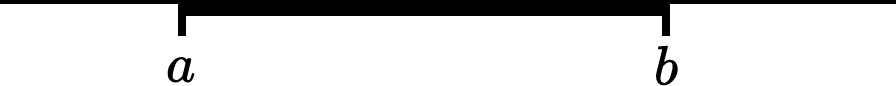
\includegraphics[width=0.4\textwidth]{images/img02.png}
	\end{center}
	Statt $a-b<0$ schreiben wir $a<b$.\\
	$a \geq b$, falls $a>b \vee a=b$\\
	$a \leq b$, falls $a<b \vee a=b$.
\end{bem}
\begin{satz}
	Sei $(\mathbb{K}, +,\cdot, >)$ ein angeordneter Körper. Dann gilt
	\begin{enumerate}
		\item für $a,b\in\mathbb{K}$ gilt genau eine der Relationen $a>b, a=b, a<b$ (Trichotromie)
		\item Aus $a>b, b>c$ folgt $a>c$ (Transitivität)
		\item Aus $a>b$ folgt:\\
		$\begin{cases}
			a+c>b+c, \forall c\in\mathbb{K}\\
			ac>bc, \text{ falls } c>0\\
			ac<bc, \text{ falls } c<0
		\end{cases}$.
		\item Aus $a>b$ und $c>d$ folgt:\\
		$\begin{cases}
			a+c>b+d\\
			ac>bd, \text{ falls } b,d>0 %WARUM FALLS b,d>0???
		\end{cases}$
		\item Für $a\neq 0$ ist $a^2 >0$.
		\item Aus $a>0$ folgt $\frac{1}{a}>0$.
		\item Aus $a>b>0$ folgt $0<\frac{1}{a}<\frac{1}{b}$.
		\item Aus $a>b, 0<\lambda<1$ folgt $b<\lambda b + (1-\lambda)a<a$.
	\end{enumerate}
\end{satz}
\begin{bem}
	Auf $\mathbb{F}_2$ kann es keine Anordnung geben!
\end{bem}
\begin{bew}
	\begin{enumerate}%schlecht formatiert
		\item Direkt aus (A.1) und Def. von $a>b$.
		\item $a-c = \underbrace{(a-b)}_{>0}+\underbrace{(b-c)}_{>0} \overset{\text{(A.2)}}{>} 0$.
		\item $(a+c)-(b+c)=a-b>0\\
		ac-bc=\underbrace{(a-b)}_{>0}\cdot c \overset{\text{(A.2)}}{>}0$, falls $c>0$\\
		Ist $c<0$, so ist $-c>0\\
		\Rightarrow bc-ac=\underbrace{(a-b)}_{>0}\cdot\underbrace{(-c)}_{>0} \overset{\text{(A.2)}}{>} 0$\\
		$ac-bd=ac-bc+bc-bd=\underbrace{(a-b)}_{>0} \cdot \underbrace{c}_{>0} + \underbrace{b}_{>0} \cdot \underbrace{(c-d)}_{>0} \overset{\text{(A.2)}}{>}0$.
		\item $(a+c)-(b+d) = (a-b)+(c-d)>0$ nach (A.2)\\
		$ac-bd = ac-bc + bc-bd = (a-b)c + b(c-d)$\\
		Ist $b=0 \Rightarrow a> b = 0 \Rightarrow ac > 0 = bd$\\
		Ist $b<0 \Rightarrow (-b)d > 0 \Rightarrow -bd > 0 \Rightarrow bd < 0 \Rightarrow ac<-bd \Rightarrow \underbrace{ac}_{>0} + \underbrace{(-bd)}_{>0} \overset{\text{(A.2)}}{>} 0$.
		\item  Fallunterscheidung:\\
		ist $a>0\Rightarrow a^2 = a\cdot a > 0$ (A.2)\\
		ist $a<0\Rightarrow a^2 = (-a)\cdot(-a) > 0$ (A.2)
		\item sei $a>0:$\\
		$\overset{\text{5.}}{\Rightarrow} \left(\frac{1}{a}\right) > 0 \Rightarrow \frac{1}{a} = \underbrace{\left(\frac{1}{a}\right)^2}_{>0} \cdot \underbrace{a}_{>0} > 0$.
		\item aus $a>b>0\\
		\Rightarrow \frac{1}{b} - \frac{1}{a} = \frac{1}{b}(a-b)\frac{1}{a}>0$.
		\item $a>b, 0>\lambda>1 \Rightarrow \lambda > 0 \wedge 1-\lambda > 0\\
		b=\lambda b + \underbrace{(1-\lambda)b}_{<(1-\lambda)a}\\
		<\lambda b + (1-\lambda) a < \lambda a + (1-\lambda)a = a\\
		\Rightarrow b<\lambda b + (1-\lambda)a =a$.\\
		Insbesondere $\lambda = \nicefrac{1}{2}\Rightarrow b< \nicefrac{1}{2} b + \nicefrac{1}{2}a = \frac{a+b}{2} < a$.
	\end{enumerate}
\end{bew}
\begin{defi}[Betrag]
	Sei $(\mathbb{K}, +,\cdot,>)$ ein angeordneter Körper.\\
	Betrag von $a\in\mathbb{K}$ ist gegeben durch\\
	$\left| a\right| := 
	\begin{cases}
		a, \text{ falls } a\geq 0\\
		-a, \text{ falls }a<0
	\end{cases}$\\
	auch noch $a,b\in \mathbb{K}$\\
	$\max(a,b) := 
	\begin{cases}
		a, \text{ falls } a\geq b\\
		b, \text{ falls } a < b
	\end{cases}\\
	\min(a,b) := 
	\begin{cases}
		a, \text{ falls } a\leq b\\
		b, \text{ falls } a > b
	\end{cases}$\\
\end{defi}
\begin{bem} . %SCHLECHT FORMATIERT
	\begin{enumerate}
		\item $a,b\in \mathbb{K}\\
		\left| a-b\right| = $ Abstand von $a$ zu $b$.\\
		$\left| a\right| = \left| a-0\right| = $ Abstand von $a$ zu $0$.
		\item $\left| a\right| = \max(a, -a)$.
	\end{enumerate}
\end{bem}
\begin{satz}
	$(\mathbb{K},+,\cdot,>)$ ang. Körper\\
	Dann gilt $\forall a,b\in\mathbb{K}:$
	\begin{enumerate}
		\item $\left|-a\right| = \left| a\right|$ und $a\leq\left|a\right|$
		\item $\left| a\right| \geq 0$ und $\left| a\right| = 0 \Leftrightarrow a = 0$
		\item $\left| ab\right| = \left| a\right| \left| b\right|$
		\item $\left| a+b\right| \leq \left| a\right| + \left|b\right|$ (Dreiecksungleichung)
		\item $\left|\left|a\right|-\left|b\right|\right| \leq \left| a-b\right|$ (umgekehrte Dreiecksungleichung)
	\end{enumerate}
\end{satz}
\begin{bew} . %SCHLECHT FORMATIERT
	\begin{enumerate}
		\item $\left| -a \right| = 
		\begin{cases}
			-a, -a \geq 0 \\
			-(-a), -a \leq 0
		\end{cases}
		= \begin{cases}
			-a, a \leq 0\\
			a, a \geq 0
		\end{cases}
		= \left| a\right|\\
		\left|a\right| - a=\begin{cases}
			a-a,a\geq 0\\
			-a-a, a<0
		\end{cases}
		= \begin{cases}
			0, a \geq 0\\
			-(a+a), a<0
		\end{cases} \geq 0$.\\
		alternativ: $a \leq \max(a, -a) = \left|a\right|$.
		\item 
		\item Hier ändern sich die linke und rechte Seite \underline{nicht}, wenn man $a$ bzw. $b$ durch $-a$ bzw. $-b$ ersetzt.\\
		Also, o.B.d.A. können wir annehmen, dass $a,b \geq 0$.\\
		$\Rightarrow \left| ab\right| = ab = \left|a\right|\left|b\right|$.
		\item $\overset{\text{Satz 1 (5)}}{\Rightarrow} \left| a+b\right|^2 = (a+b)^2=a^2+2ab+b^2=\left|a\right|^2 + 2\underbrace{ab}{\leq \left| ab\right|} + \left|b\right|^2\\
		\overset{\text{(2)}}{\leq} \left|a\right|^2 + 2\left|ab\right| + \left|b\right|^2\\
		\overset{\text{(3)}}{\left|a\right|^2+2\left|a\right|\left|b\right| + \left|b\right|^2}$.\\
		Also $(a+b)^2 \leq (\left|a\right| + \left| b\right|)^2\\
		\overset{\text{H.A.}}{\Rightarrow}\left|a+b\right| \leq \left|a\right|+\left|b\right|$.\\
		H.A. aus $\left|c\right|^2 \leq \left|d\right|^2$ folgt $|c| \leq |d|$ (Kontraposition).
		\item $|a| = \left| a-b+b\right| = \left| (a-b) + b\right| \overset{\text{(4)}}{\leq} \left|a-b\right| + |b|\\
		|a|-|b|\leq \left|a-b\right| \forall a,b\in\mathbb{K}$.\\
		Jetzt: Symmetrieargument. (Vertausch von $a$ und $b$)\\
		$\Rightarrow |b| - |a| \leq \left|b-a\right| = \left|(-b-a)\right| = \left|a-b\right|$\\
		also $|b|-|a| \leq \left|a-b\right|\\
		|a|-|b| \leq \left|a-b\right|\\
		\left| |a|-|b|\right| = \max(\left|a\right|-\left|b\right|, -(|a|-|b|))=\max(|a|-|b|, |b|-|a|) \leq |a-b|$.
	\end{enumerate}
\end{bew}
\begin{bsp}
	Sei $a,b\in\mathbb{K}$ ein angeordneter Körper. Aus $|b-a|\leq \nicefrac{b}{2}, 2 = 1+1$ folgt $a \geq \nicefrac{b}{2}$
	Bild: %BILD EINFUEGEN\\
	\begin{bew}
		$b-a \leq |b-a| \leq \nicefrac{b}{2} \Rightarrow a \geq b - \nicefrac{b}{2} = \nicefrac{b}{2}$.
	\end{bew}
\end{bsp}
\begin{kor}[\glqq geometrisch-arithmetische Ungleichung\grqq]
	Sei $(\mathbb{K},+,\cdot,>)$ ein ang. Körper, $a,b\in\mathbb{K}\\
	\Rightarrow ab \leq \left( \dfrac{a+b}{2}\right)^2$.\\
	Wenn Gleichheit gilt, so folgt $a=b$.
\end{kor}
\begin{bew}
	In Übung
\end{bew}
\textbf{Fakt:}
\begin{itemize}
	\item In jedem angeordneten Körper gilt $0<1$!
	\item Es gibt keine Anordnung, die $\mathbb{F}_2$ zu einem angeordneten Körper macht. (H.A.)
\end{itemize}
\subsection{Obere und untere Schranken, Supremum und Infimum}
Notation: $a$ ist nicht negativ, falls $a\geq 0$.
\\natürlich $a=b\Leftrightarrow a\leq b \wedge a \geq b$.\\
Im Folgenden ist $\mathbb{K}$ immer ein angeordneter Körper. $A,B \subset \mathbb{K}, A,B\neq \emptyset$ und $\gamma \in \mathbb{K}$, so bedeutet $A\leq \gamma: \forall a\in A: a \leq \gamma$ ($\gamma$ it obere Schranke für $A$).\\
$B\geq \beta: \forall b\in B: b\geq \beta$ ($\beta$ ist untere Schranke für $B$).\\
Analog sind $a<\gamma, A>\gamma, A<B,$ usw. definiert.\\
Hat $A$ eine obere Schranke, so heißt $A$ nach oben beschränkt. Hat $B$ eine untere Schranke, so ist $B$ nach unten beschränkt. $A$ ist beschränkt, falls es nach oben und unten beschränkt ist.\\
Ist $A\leq \alpha$ und $\alpha\in A$, so heißt $\alpha$ größtes (maximales) Element von $A$, schreibe $\alpha = \max A$ (Maximum).\\
Ist $B\geq \beta$ und $\beta\in B$, so heißt $B$ kleinstes (minimales) Element von $B$, schreibe $\beta = \min B$ (Minimum).\\
Man zeige, dass $\max$ und $\min$ eindeutig sind, sofern sie existieren.\\
$[0,1) := \{x\in\mathbb{K}|0\leq x\leq 1\}$ hat kein Maximum bzw. kein maximales Element.
\begin{defi}
	Sei $A\subset \mathbb{K}, A\neq \emptyset$. Dann ist $\gamma\in\mathbb{K}$ die kleinste obere Schranke (oder Supremum), falls $A\leq \gamma$ und aus $A\leq n$ folgt $\gamma \leq n$.\\
	Schreibe $\gamma = \sup A = \sup(A)$.\\
	Analog: $\beta$ it die größte untere Schranke von $A$ (Infimum), falls $\beta \leq A$ und aus $\eta \leq A$ folgt $\eta \leq \beta$\\
	Schreibe $\beta = \inf A = \inf(A)$.
\end{defi}
\begin{bsp}
	$P := \{x\in\mathbb{K}|x>0\}\\
	\Rightarrow$
	\begin{enumerate}
		\item $P$ ist nicht nach oben beschränkt.
		\item $P$ hat kein Minimum, aber $\inf P = 0$.
	\end{enumerate}
\end{bsp}
\begin{bew} . %Schlecht formatiert
	\begin{enumerate}
		\item Ang. $\gamma$ ist obere Schranke für $P$. D.h. $\forall x\in P$ folgt $0<x\leq\gamma\Rightarrow\gamma >0\Rightarrow \gamma \in P \Rightarrow 0 < \gamma = \gamma + 0 < \gamma + 1 \in P\Rightarrow\gamma + 1\in P$ und $\gamma +1>\gamma \gamma$ ist nicht obere Schranke für $P$ (Widerspruch!) \Lightning
		\item $2:= 1+1 > 1>0$\\
		Ang. $\min P := \eta$ existiert. $\Rightarrow \eta \in P, \eta > 0, \tilde{x} := \frac{\eta}{2} = \frac{0 + \eta}{2} < \eta$.\\
		Es gilt $0 = \inf P$.\\
		Sicherlich $0<P$, also ist $0$ eine untere Schranke für $P$.\\
		$0$ ist die größte untere Schranke, denn nach obigem Argument ist jede Zahl $>0$ keine untere Schranke für $P$!
	\end{enumerate}
\end{bew}
\begin{lem}
	$A\subset\mathbb{K}, A\neq \emptyset$.
	\begin{enumerate}
		\item $\alpha := \sup A \Leftrightarrow \alpha \geq A \wedge \forall \varepsilon > 0 \exists a \in A: \alpha - \varepsilon < a$.
		\item $\beta := \inf B \Leftrightarrow \beta \leq B \wedge \forall \varepsilon > 0 \exists b \in B: b < \beta + \varepsilon$.
	\end{enumerate}
\end{lem}
\begin{bew} .%SCHLECHT FORMATIERT
	\begin{enumerate}
		\item \glqq $\Rightarrow$\grqq: Sei $\alpha = \sup A$. Also $\alpha$ ist die kleinste obere Schranke für $A$. D.h. $\alpha \geq A$ und $\forall \varepsilon > 0$ ist $\varepsilon>0<\alpha$, also ist $\alpha-\varepsilon$ keine obere Schranke für $A$. D.h. $\exists a\in A:\alpha - \varepsilon <a$.\\
		\glqq $\Leftarrow$\grqq: Sei $\alpha \geq A \wedge \forall \varepsilon > 0 \exists a \in A: \alpha - \varepsilon < a$. Also ist $\alpha$ eine obere Schranke für $A$. Sei $\tilde{\alpha}<\alpha$.\\
		Setze $\varepsilon:= \alpha -\tilde{\alpha} > 0 \Rightarrow \exists a \in A: \tilde{\alpha} = \alpha - \varepsilon < a \Rightarrow \tilde{\alpha}$ ist keine obere Schranke für $a$. $\Rightarrow\alpha$ ist die kleinste obere Schranke.
		\item $A:= -B = \{-b|b \in B\}$. Beachte: $\sup A = \sup(-B) = -\inf B$.
	\end{enumerate}
\end{bew}
%30.10.2018
\subsection{Das Vollständigkeitsaxiom}
\begin{defi}
	Ein angeordneter Körper $(\mathbb{K},+,\cdot,>)$ erfüllt das Vollständigkeitsaxiom, falls\\
	\begin{center}
		Jede nichtleere, nach oben beschränkte Teilmenge hat ein Supremum.
	\end{center}
	Solch einen Körper nennt man ordnungsvollständig. $\mathbb{R}$, der Körper der reellen Zahlen, ist \underline{der} ordnungsvollständige Körper. (Im Wesentlichen gibt es nur einen!)
\end{defi}
$\mathbb{Q}; A:= \{r\in\mathbb{Q}|r^2 < 2\}$\\
Notation: $a,b\in\mathbb{R} \quad a<b$\\
$[a,b] := \{x\in\mathbb{R}|a\leq x\leq b\}$ abgeschlossenes Intervall\\
$(a,b) := \{x\in\mathbb{R} | a<x<b\}$ offenes Intervall\\
$[a,b) := \{x\in\mathbb{R}|a\leq x<b\}$ nach rechts halboffenes Intervall\\
$(a,b] := \{x\in\mathbb{R}|a<x\leq b\}$ nach links halboffenes Intervall\\
Intervalllänge: $b-a$\\
unbeschränkte Intervalle:\\
$(-\infty, a] := \{x\in\mathbb{R}|x\leq a\}$\\
$[a,\infty) := \{x\in\mathbb{R}|x\geq a\}$\\
$(-\infty, a) := \{x\in\mathbb{R}|x<a\}$\\
$(a, \infty) := \{x\in\mathbb{R}|x>a\}$.
\subsection{Die natürlichen Zahlen $\mathbb{N}$}
(als Teilmenge von $\mathbb{R}$)\\
$n$ natürliche Zahl, $n=\underbrace{1+1+\ldots + 1}_{n\text{-mal}}$ (zirkulär \Lightning)
\begin{defi}
	Eine Teilmenge $M\subset \mathbb{R}$ heißt \underline{induktiv}, falls
	\begin{enumerate}
		\item $1\in M$
		\item Aus $x\in M$ folgt $x+1 \in M$
	\end{enumerate}
\end{defi}
\begin{bsp}
	$[1,\infty)$ ist induktiv.\\
	$\mathbb{R}$ ist induktiv.\\
	$(1,\infty)$ ist nicht induktiv.\\
	$\{1\} \cup [1+1,\infty)$ ist induktiv.
\end{bsp}
\textbf{Beobachtung:} Ein beliebiger Schnitt induktiver Mengen ist wieder induktiv.\\
$J$: Indexmenge $A_0$ induktiv $\forall j\in J$\\
$\Rightarrow \forall i\in J: 1\in A_j \Rightarrow 1\in \underset{j\in J}{\bigcap} A_j$\\
Ist $x\in \underset{j\in J}{\bigcap} A_j\Rightarrow \forall j \in J: x\in A_j \Rightarrow x+1 \in A_j \Rightarrow x+1 \in \underset{j\in J}{\bigcap} A_j$.
\begin{defi}[natürliche Zahlen] .\\ %SCHLECHT FORMATIERT
	$\mathbb{N} := \{x\in \mathbb{R}: \text{ für jede induktive Teilmenge } M\in\mathbb{R} \text{ gilt } x\in M\} := \underset{M\subset \mathbb{R}\text{ ist induktiv}}{\bigcap} M$
\end{defi}
\begin{bem}
	$\mathbb{N}$ ist induktiv und $\mathbb{N}$ ist die kleinste induktive Teilmenge von $\mathbb{R}$.
\end{bem}
\begin{satz}[Archimedisches Prinzip für $\mathbb{R}$] .%SCHLECHT FORMATIERT
	\begin{enumerate}
		\item $\mathbb{N}$ ist (in $\mathbb{R}$) \underline{nicht} nach oben beschränkt!
		\item $\forall x\in\mathbb{R}$ mit $x>0 \exists n\in \mathbb{N}: \frac{1}{n} < x$.
	\end{enumerate}
\end{satz}
\begin{bew}
	\begin{enumerate}
		\item Angenommen, $\mathbb{N}\subset{R}$ ist nach oben beschränkt.\\
		$\mathbb{N} \neq \emptyset$ (da $1\in\mathbb{N}$)\\
		Vollständigkeitsaxiom $\Rightarrow \alpha := \sup \mathbb{N} \in \mathbb{R}$.\\
		Setze $\varepsilon = 1$ in Lemma 3.3.2\\ %NOCH VERKNÜPFUNG EINFÜGEN
		$\alpha -1$ ist nicht obere Schranke für $\mathbb{N}$.\\
		$\exists n\in \mathbb{N}: n>\alpha-1\\
		\Rightarrow n+1 > \alpha \in \mathbb{N}$ \Lightning  zu $\alpha$ ist obere Schranke von $\mathbb{N}$.
		\item Sei $x>0 \overset{\text{Satz 3.2.1 (6)}}{\Rightarrow} \frac{1}{x} > 0\Rightarrow \exists n\in \mathbb{N}: n > \frac{1}{x}\underset{\text{Satz 3.2.1 (7)}}{\Rightarrow} x = \dfrac{1}{\nicefrac{1}{x}} > \frac{1}{n}$. %VERLINKUNGEN ZU SÄTZEN
	\end{enumerate}
\end{bew}
\begin{satz}[Induktionsprinzip]
	Sei $M\subset \mathbb{N}$ mit 
	\begin{enumerate}
		\item $1\in M$
		\item Ist $x\in M \Rightarrow x+1 \in M$
	\end{enumerate}
	Dann ist $M= \mathbb{N}$.
\end{satz}
\begin{bew}
	$\Rightarrow M$ ist induktiv. $\mathbb{N}$ kleinste induktive Teilmenge von $\mathbb{R}$\\
	$\Rightarrow \mathbb{N} \subset M$\\
	$M\subset \mathbb{N} \wedge \mathbb{N} \subset M \Leftrightarrow M = \mathbb{N}$.
\end{bew}
\begin{kor}[Vollständige Induktion]
	Für $n\in\mathbb{N}$ seien $A(n)$ Aussagen.
	Es gelte:
	\begin{enumerate}
		\item $A(1)$ ist wahr.
		\item aus $A(n)$ ist wahr folgt $A(n+1)$ ist wahr.
	\end{enumerate}
\end{kor}
\begin{bew}
	Definiere $M := \{n\in \mathbb{N}| A(n) \text{ ist wahr}\} \subset \mathbb{N}$.
	\begin{enumerate}
		\item $\Rightarrow 1\in M$, da $A(1)$ wahr ist
		\item $\Rightarrow$ sei $n\in M$, d.h. $A(n)$ ist wahr $\Rightarrow A(n+1)$ ist wahr, d.h. $n+1\in M$.
	\end{enumerate}
	$\overset{\text{Ind.prinzip Satz 4}}{\Rightarrow} M = \mathbb{N}$, also sind alle $A(n)$ wahr! %LINK ZU SATZ 4!
\end{bew}
Notation: Induktive Definition von Summen und Produkten.\\
$a_1+a_2+\ldots + a_n$ vage \dots\\
\textbf{Summe:} \[\sum_{k=1}^{1} a_k := a_1, (n = 1), \sum_{k=1}^{n+1} a_k := \left( \sum_{k=1}^{n} a_k\right) + a_{n+1}, n\in\mathbb{N}\]
Allgemein: untere Grenze $k=m$, obere Grenze $k=n$, Laufindex kann verschoben werden.\\
z.B.: $k= j+1$
\[\sum_{k=m}^{n}a_k = \sum_{j=m-1}^{n-1}a_{j+1} = \ldots = \sum_{l = 0}^{n-m}a_{l+m}\]
Ist $m>n$, definieren $\sum_{k=m}^{n-m}a_k := 0$ (leere Summe)\\
\textbf{Produkt:} $$\prod_{k=1}^{1}a_k := a_1, \prod_{k=1}^{n+1}a_k := \left( \prod_{k=1}^{n}a_k\right) \cdot a_{n+1}, n\in\mathbb{N}$$
Ähnlich $\prod_{k=m}^{n}a_n$, setzen für $m>n \prod_{k=m}^^n a_k := 1$ (leeres Produkt)\\
z.B. $$a\in\mathbb{R}, a^n = \prod_{k=1}^n a \text{, d.h. } a^1=a, a^{n+1} = a^n \cdot a, n\in\mathbb{N} \text{ (induktive Definition)}$$
Rechenregeln gelten z.B. $$\sum_{k=1}^{n} (a_k+b_k) = \sum_{k=1}^{n} a_k + \sum_{k=1}^{n} b_k\\
a_j, b_j \in\mathbb{R}, j=1,\ldots, n$$
$$c \in\mathbb{R}, \sum_{n}^{k=1} (c\cdot a_k) = c\cdot \sum_{k=1}^{n} a_k$$
\begin{satz}[Bernoullische Ungleichung]
	$$x\in\mathbb{R}, x\geq -1, n\in\mathbb{N}_0 = \mathbb{N}\cup \{0\}$$
	gilt $(1+x)^n \geq 1+ n + x (\forall m\in\mathbb{N},x\geq -1)$\\mit \glqq $>$\grqq, falls $n>1, x\neq 0$\\
	$( \forall n\in\mathbb{N}, x \geq -1(1+x)^n \geq 1 + nx)$
\end{satz}
\begin{bew}
	Vollständige Induktion:\\
	Induktionsanfang:
	$$n=0: (1+x)^0=1=1+0x \checkmark$$
	$$n=1: (1+x)^1=1+x=1+1x \checkmark$$
	Induktionsschritt:
	Induktionsvoraussetzung: es gelte für ein festes, aber beliebiges $n\in\mathbb{N}$: 
	\begin{equation*}
	\begin{aligned}
		(1+x)^n &\geq 1+nx\\%LINEBREAK KLAPT NICHT
		(1+x)^{n+1} &= \underbrace{(1+x)^{n}}_{\geq 1+nx} \cdot \underbrace{(1+x)}_{> 0} \geq (1+nx)(1+x) = 1+(n+1)x + nx^2\\
		&=\begin{cases}
		\geq 1+(n+1)x, x>-1\\
		> 1+(n+1)x, x>-1, x\neq 0
		\end{cases}
	\end{aligned}
	\end{equation*}
\end{bew}
\begin{satz}[geometrische Summe]
	Sei $x\neq 1$, dann ist $$\sum_{k=0}^{n}x^k = \frac{1-x^{n+1}}{1-x}$$
\end{satz}
\begin{bew}
	Vollständige Induktion:\\
	IA:
	\begin{equation*}
	\begin{aligned}
		n=0: &\sum_{k=0}^{0} x^k = x^0 = 1 = \frac{1-0}{1+0}\checkmark\\
		n=1: &\sum_{n=0}^{1} x^k = 1+x = \frac{1-x}{1-x} (1+x) = \frac{1-x^2}{1-x}\checkmark
	\end{aligned}
	\end{equation*}
	IS:\\
	IV: Es gelte für ein festes, aber beliebiges $n\in\mathbb{N}$: $$\sum_{k=0}^{n} x^k = \frac{1-x^{n+1}}{1-x}$$
	\begin{equation}
		\begin{aligned}
		\Rightarrow \sum_{k=0}^{n} x^k + x^{n+1} \overset{\text{IV}}{=} \frac{1-x^{n+1}}{1-x} + x^{n+1}\\
		= \frac{1-x^{n+1} + (1-x)x^{n+1}}{1-x} = \frac{1-x^{n+2}}{1-x}.
		\end{aligned}
	\end{equation}
\end{bew}
\begin{bew} ohne vollständige Induktion:
	\[
	\begin{aligned}
		S_n &:= \sum_{k=0}^{n} x^k\\
		x\cdot S_n &= \sum_{k=0}^{n} x^k = \sum_{k=0}^{n} x^{k+1} = \sum_{j=1}^{n+1} x^j,\\
		\Rightarrow (1-x)S_n &= S_n - x S_n = \sum_{k=0}^{n} x^k - \sum_{k=1}^{n+1} x^k = x^0 - x^{n+1} = 1-x^{n+1}\\
		\Rightarrow S_n &= \frac{1-x^{n+1}}{1-x}
	\end{aligned}\]
\end{bew}
\begin{satz}[Eigenschaften von $\mathbb{N}$]
	Es gilt
	\begin{enumerate}
		\item $\forall m,n \in \mathbb{N}: n+m \in \mathbb{N}$ imd $n\cdot m \in \mathbb{N}$.
		\item $\forall n\in\mathbb{N}: n=1$ oder $(n>1$ und demnach $n-1 \in \mathbb{N})$.
		\item $\forall m,n\in\mathbb{N}:m\leq n:n-m\in\mathbb{N}_0$.
		\item $\forall n\in\mathbb{N}$ gibt es kein $m\in\mathbb{N}: n<m<n+1$.
	\end{enumerate}
\end{satz}
\begin{bew}.%Falsch formatiert
\begin{enumerate}
	\item Gegeben $m\in\mathbb{N}: A :=\{n\in \mathbb{N}| n+m\in \mathbb{N}\}\subset \mathbb{N}$\\
	\begin{enumerate}
		\item $1\in A$, denn $m\in\mathbb{N}: 1+m = m+1\in\mathbb{N}$.
		\item Angenommen, $n\in A \Rightarrow (n+1) + m = \underbrace{n+m}_{\in\mathbb{N}} + 1 \in\mathbb{N}\\
		\Rightarrow n+1\in A$
	\end{enumerate} somit ist $A$ induktiv, also $\mathbb{N}\subset A \Rightarrow A = \mathbb{N}$.
	\item Definiere $B:= \{n\in \mathbb{N}|n=1 \vee (n-1\in\mathbb{N}\wedge n-1\geq 1)\} \subset \mathbb{N}$\\
	Dann ist $B$ induktiv, denn
	\begin{enumerate}
		\item $1\in B, 2=1+1\in B$
		\item Sei $1\neq n\in B$, so folgt $1\leq n-1$ und somit $n=(\underbrace{n-1}_{\in\mathbb{N}}) +1\in\mathbb{N}$\\
		$\Rightarrow n+1\in\mathbb{N}$ und $(n+1)-1=n\geq 1+1>1$.
		Somit ist $n+1\in B$.		
	\end{enumerate}
	\item $C:= \{n\in \mathbb{N} | \forall m \in \mathbb{N}$ mit $m\leq n$ ist $n-m\in \mathbb{N}_0\}\Rightarrow$
	\begin{enumerate}
		\item $1\in C$, denn ist $m\in \mathbb{N}$ und $m=1$.\\
		folgt nach b): $m=1$\\
		$\Rightarrow n - m = 1 - 1 = 0\in \mathbb{N}_0$.
		\item ang. $n\in C$ und $m\in\mathbb{N}$ mit $m\leq n+1$.\\
		Fallunterscheidung:
		\begin{itemize}
			\item $n=1 \Rightarrow n+1-m=(n+1)-1=n\in\mathbb{N}.\checkmark\\
			\Rightarrow n+1\in C.$
			\item $n > 1$ (und $m \leq n+1$)\\
			$\overset{\text{2.}}{\Rightarrow} m-1\in \mathbb{N}$ und $m-1 \leq (n+1)-1 = n$\\%b) unter Implikationspfeil
			Da $n\in C, m-1\in\mathbb{N}, m-1\leq n \Rightarrow \underbrace{n-(m-1)}_{=(n+1)-m} \in \mathbb{N}_0\\
			\Rightarrow n+1\in C$.
		\end{itemize}
	\end{enumerate}
	\item H.A.
\end{enumerate}
\end{bew}
%02.11.2018
\section{Funktionen und Abbildungen}
\subsection{Funktion als Abbildung}
\begin{defi}
	Eine Funktion (oder Abbildung) von einer Menge $A$ in eine Menge $B$ ordnet jedem Element $a\in A$ ein \underline{eindeutiges} Element $b \in B$ zu.\\
	Wir schreiben:
	\begin{equation*}
		f: A \rightarrow B, a \mapsto f(a)\quad(=b)
	\end{equation*}	
	$A$: Definitionsbereich\\
	$B:$ Zielbereich (Target(space))\\
	z.B. $f: \mathbb{R} \rightarrow \mathbb{R}, x \mapsto x^2$\\
	Die Abbildung $f: A \rightarrow B$ ist\\
	\begin{tabular}{r|l}
		injektiv&aus $f(a) = f(a'), a, a' \in A$, folgt $a=a'$\\
		surjektiv&$\forall b\in B \exists a\in A: b=f(a)$\\
		bijektiv&sie ist injektiv und surjektiv
	\end{tabular}
\end{defi}
\begin{bem}
	$f: A\rightarrow B$ injektiv $\Leftrightarrow a, a'\in A, a \neq a' \Rightarrow f(a) \neq f(a')$
\end{bem}
$f: A\rightarrow B$ ist bijektiv $\Rightarrow \forall b\in B \exists ! a\in A: f(a) = b$.\\
Definiere $f^{-1}: B\rightarrow A, b\mapsto a, a\in A: f(a) = b$ (inverse Funktion).\\
Ist $f: A\rightarrow B$ nicht bijektiv. (Verallgemeinerte Inverse)\\
$f^{-1}: P(B)\rightarrow P(A), M \mapsto\{a\in A|f(a)\in M\}$\\
Verkettung:\\
gegeben: $f:A\rightarrow B, g: B\rightarrow C$\\
$g\circ f: A\rightarrow C\qquad g\circ f(a):= g(f(a))$.\\
$A\overset{f}{\rightarrow} B \overset{g}{\rightarrow}C$\\
$f: A\rightarrow B$ ist bijektiv $\Rightarrow f^{-1}\circ f = \operatorname{id}_A, f\circ f^{-1} = \operatorname{id}_B$\\
$\operatorname{id}_A: A\rightarrow A, a\mapsto a.$
\subsection{Abbildungen als Graph}
\begin{defi}
	Seien $A,B$ Mengen. Dann ist $(a,b)$ ein sog. \underline{Tupel}.\\
	in der Mengenlehre: $(a,b) := \{\{a\}, \{a,b\}\}$.
\end{defi}
Beachte: Reihenfolge ist wichtig! im Allg. $(a,b)\neq (b,a)$\\
Menge $A\times B := \{(a,b)|a\in A, b\in B\}$\\
heißt kartesisches Produkt (von $A$ und $B$)\\
z.B. $\mathbb{R}\times\mathbb{R}$\\
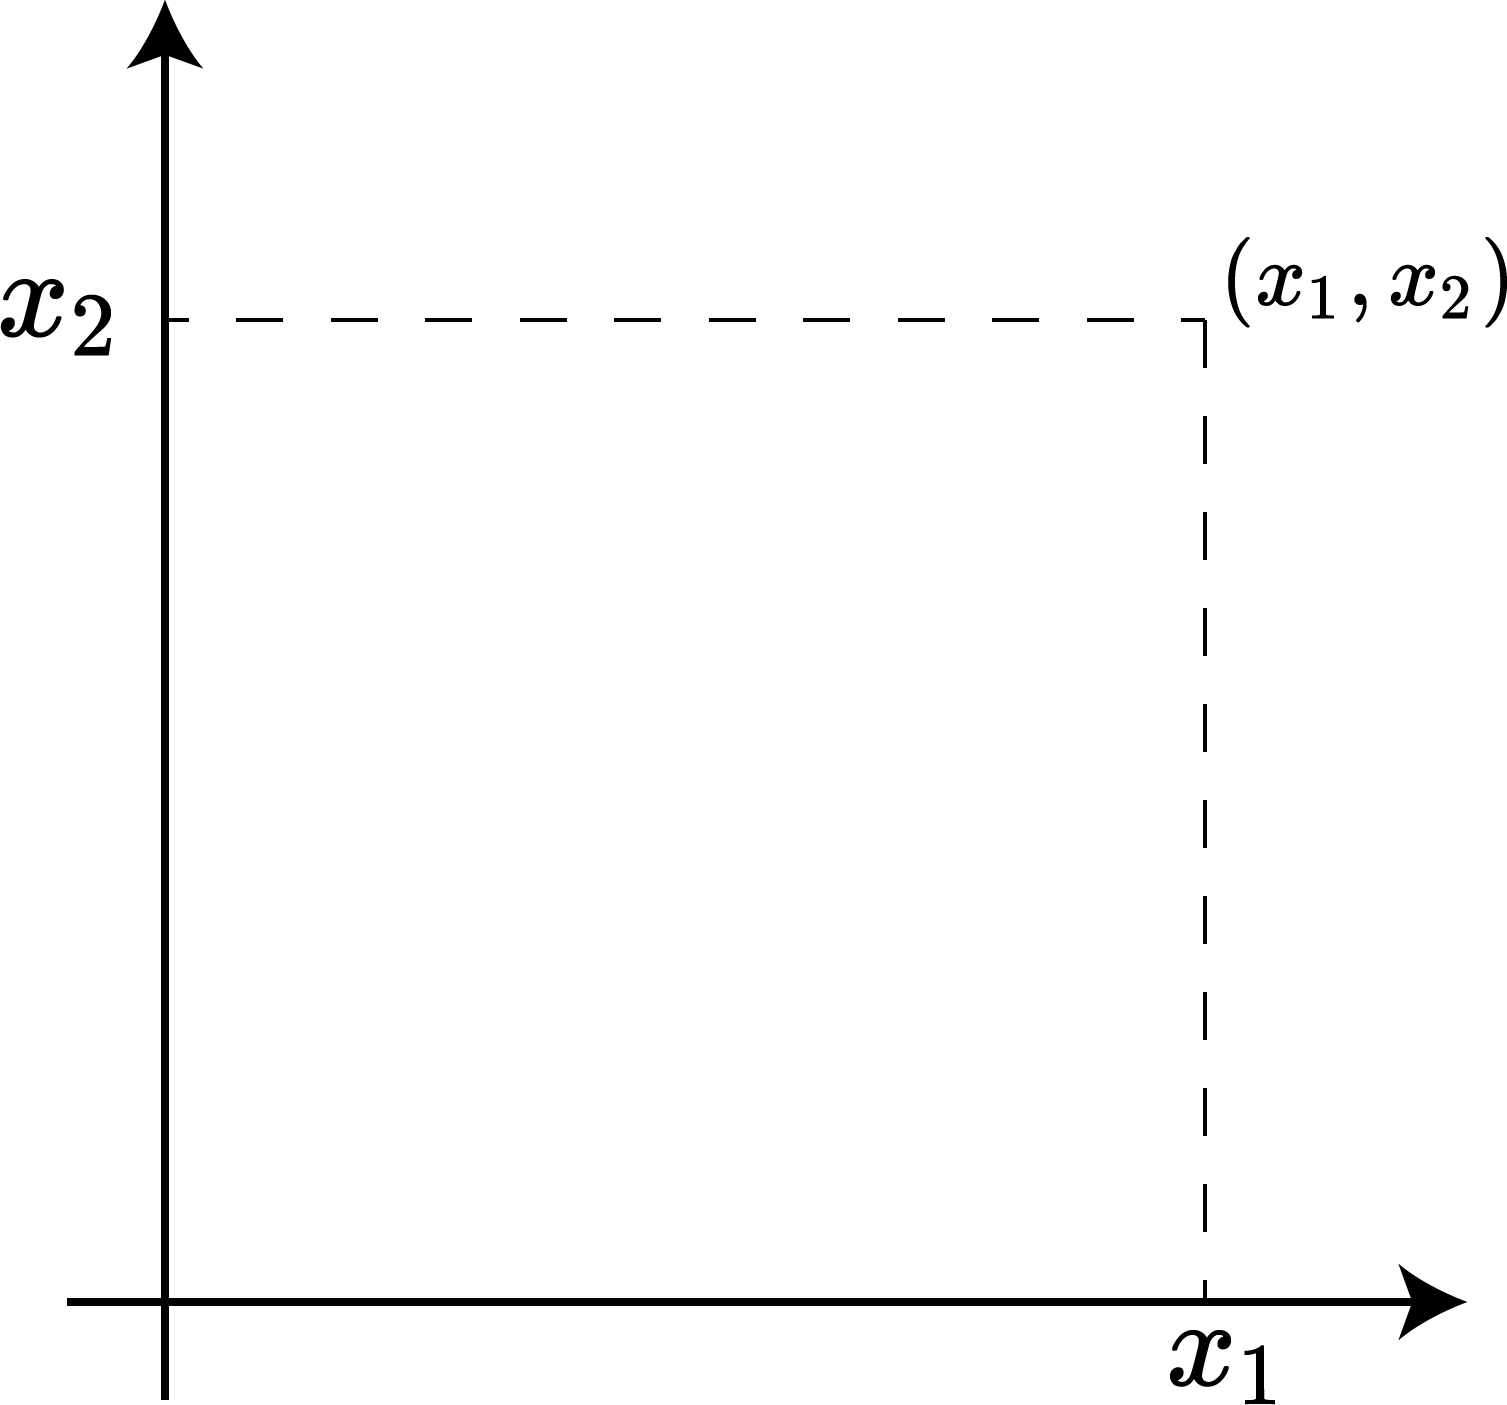
\includegraphics[width=0.3\textwidth]{images/img03.png}\\
\underline{2. Abbildungen} Projektionen\\
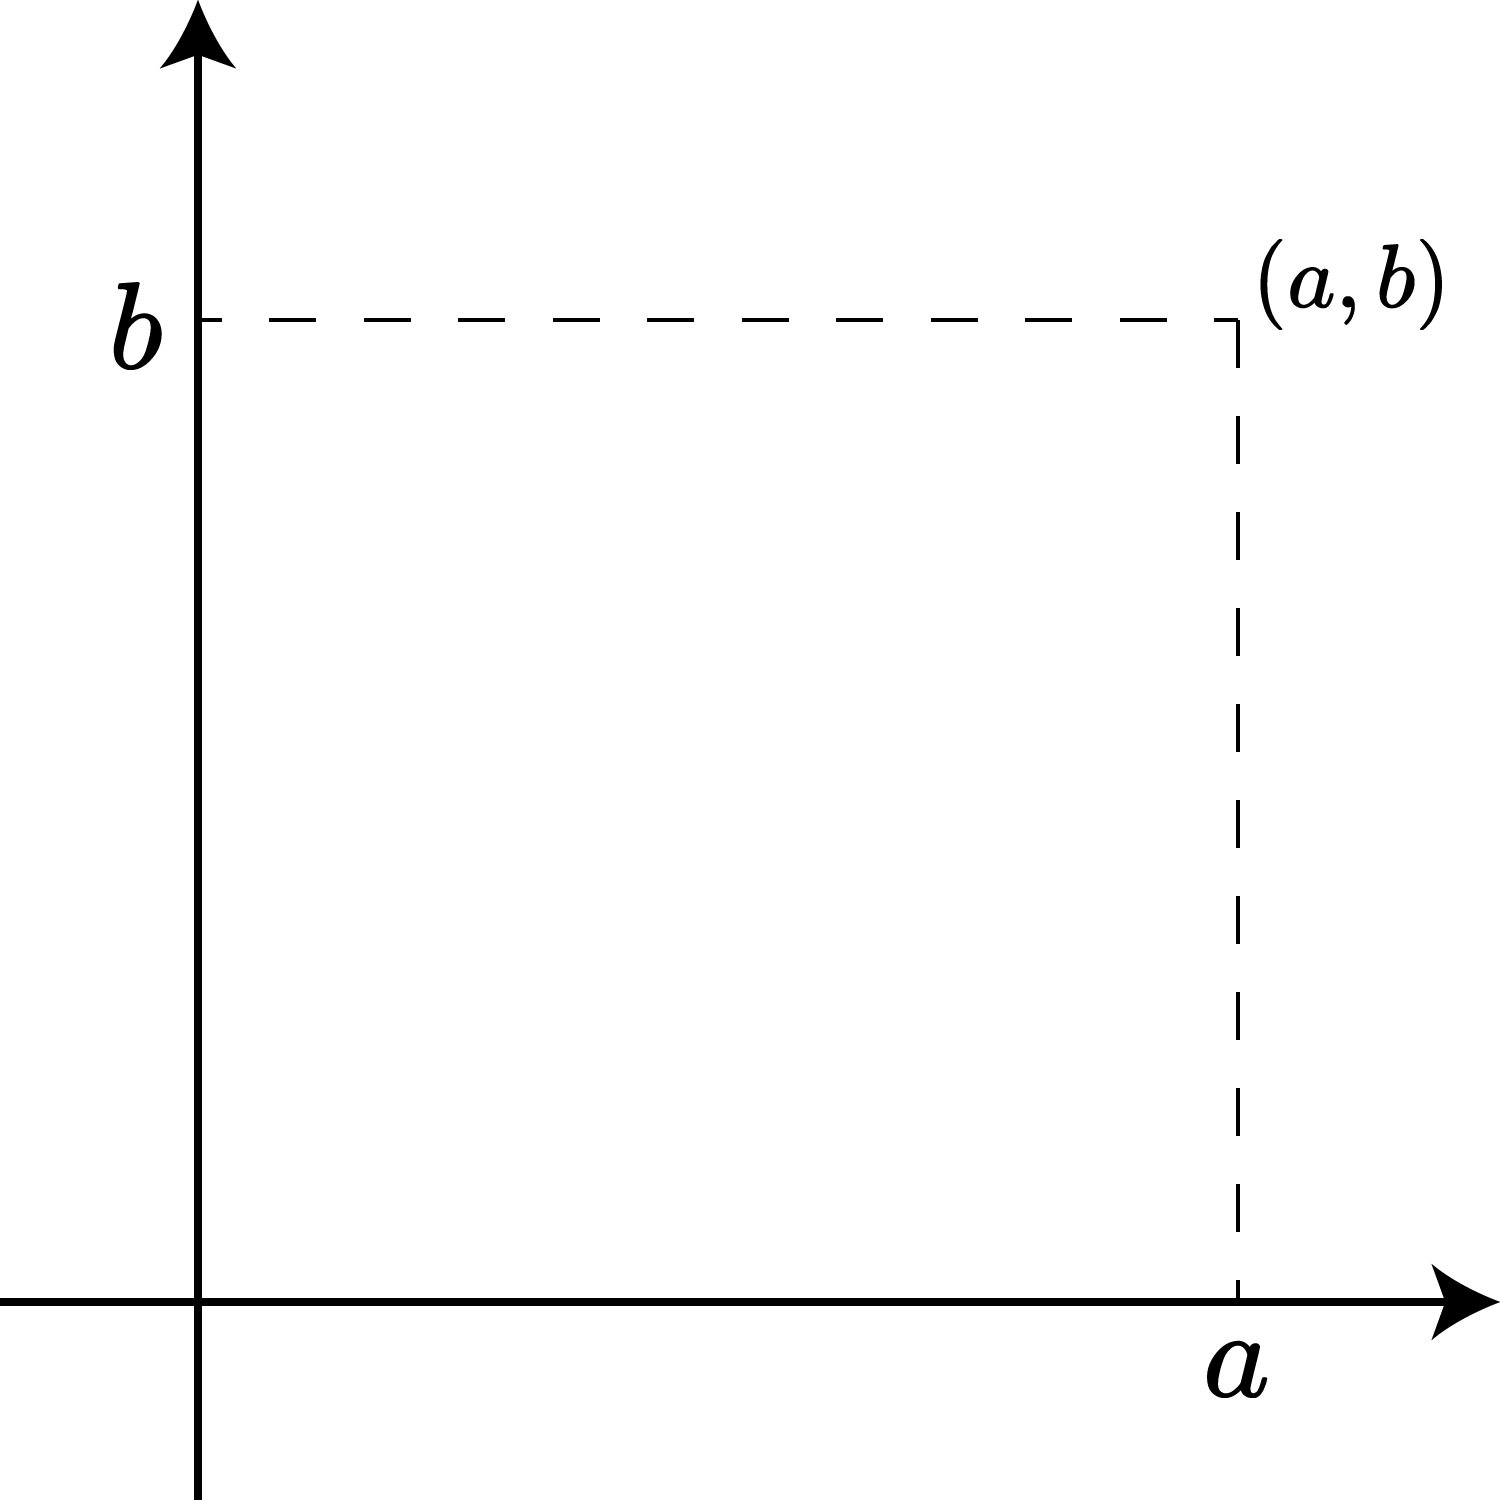
\includegraphics[width=0.3\textwidth]{images/img04.png}\\
$\Pi_1 = \Pi_A : A\times B \rightarrow A, (a,b)\mapsto a$ (Projektion auf 1. Koordinate)\\
$\Pi_2 = \Pi_B : A\times B \rightarrow B, (a,b) \mapsto b$ (Projektion auf 2. Koordinate)\\
$\Pi_A(a,b) = a$\\
$\Pi_B(a,b) = b$\\
$n$-Tupel: Mengen $A_1,\dots ,A_n, n\in \mathbb{N}.$\\
$A_1\times A_2$ wie vorhin\\
$A_1\times\dots\times A_{n+1} := (A_1\times\dots\times A_n)\times A_{n+1}, n\in \mathbb{N}$ (induktiv)\\
\underline{Beobachtung:}\\
$(A\times B)\times C = A\times (B\times C) + \{(a,b,c)|a\in A, b\in B, c\in C\} = ((a,b),c) = (a,(b,c))$\\
Genauer: $\exists$ Bijektion $\Phi : (A\times B) \times C \rightarrow A\times (B\times C)$

\begin{defi}[Graph einer Abbildung]
	Geg: $f: A \rightarrow B$ Funktion\\
	$\Gamma := \Gamma_f := \{(a,b) \in A\times B : b = f(a)\} \subset A\times B$\\
	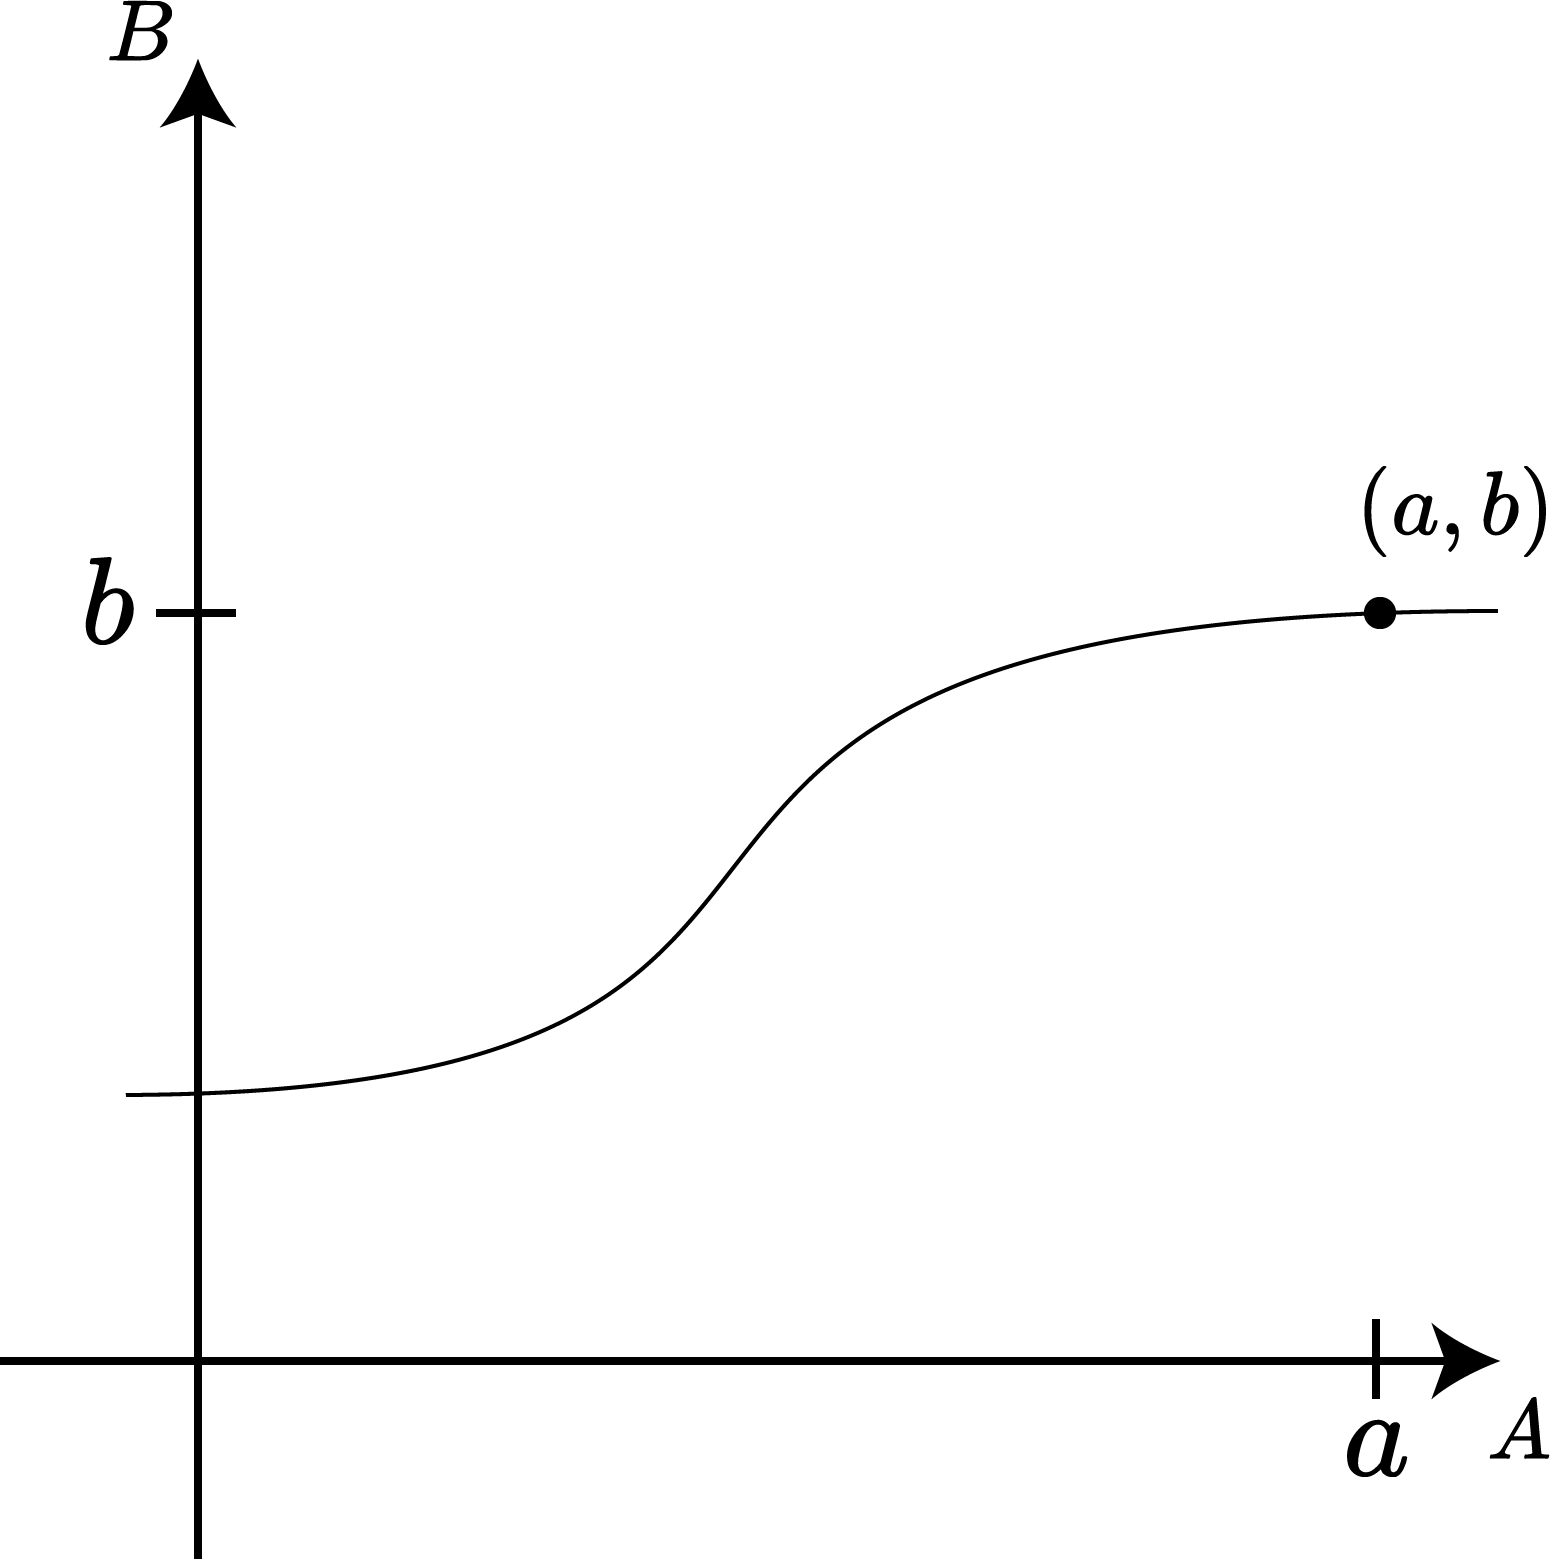
\includegraphics[width=0.3\textwidth]{images/img05.png}
	\quad
	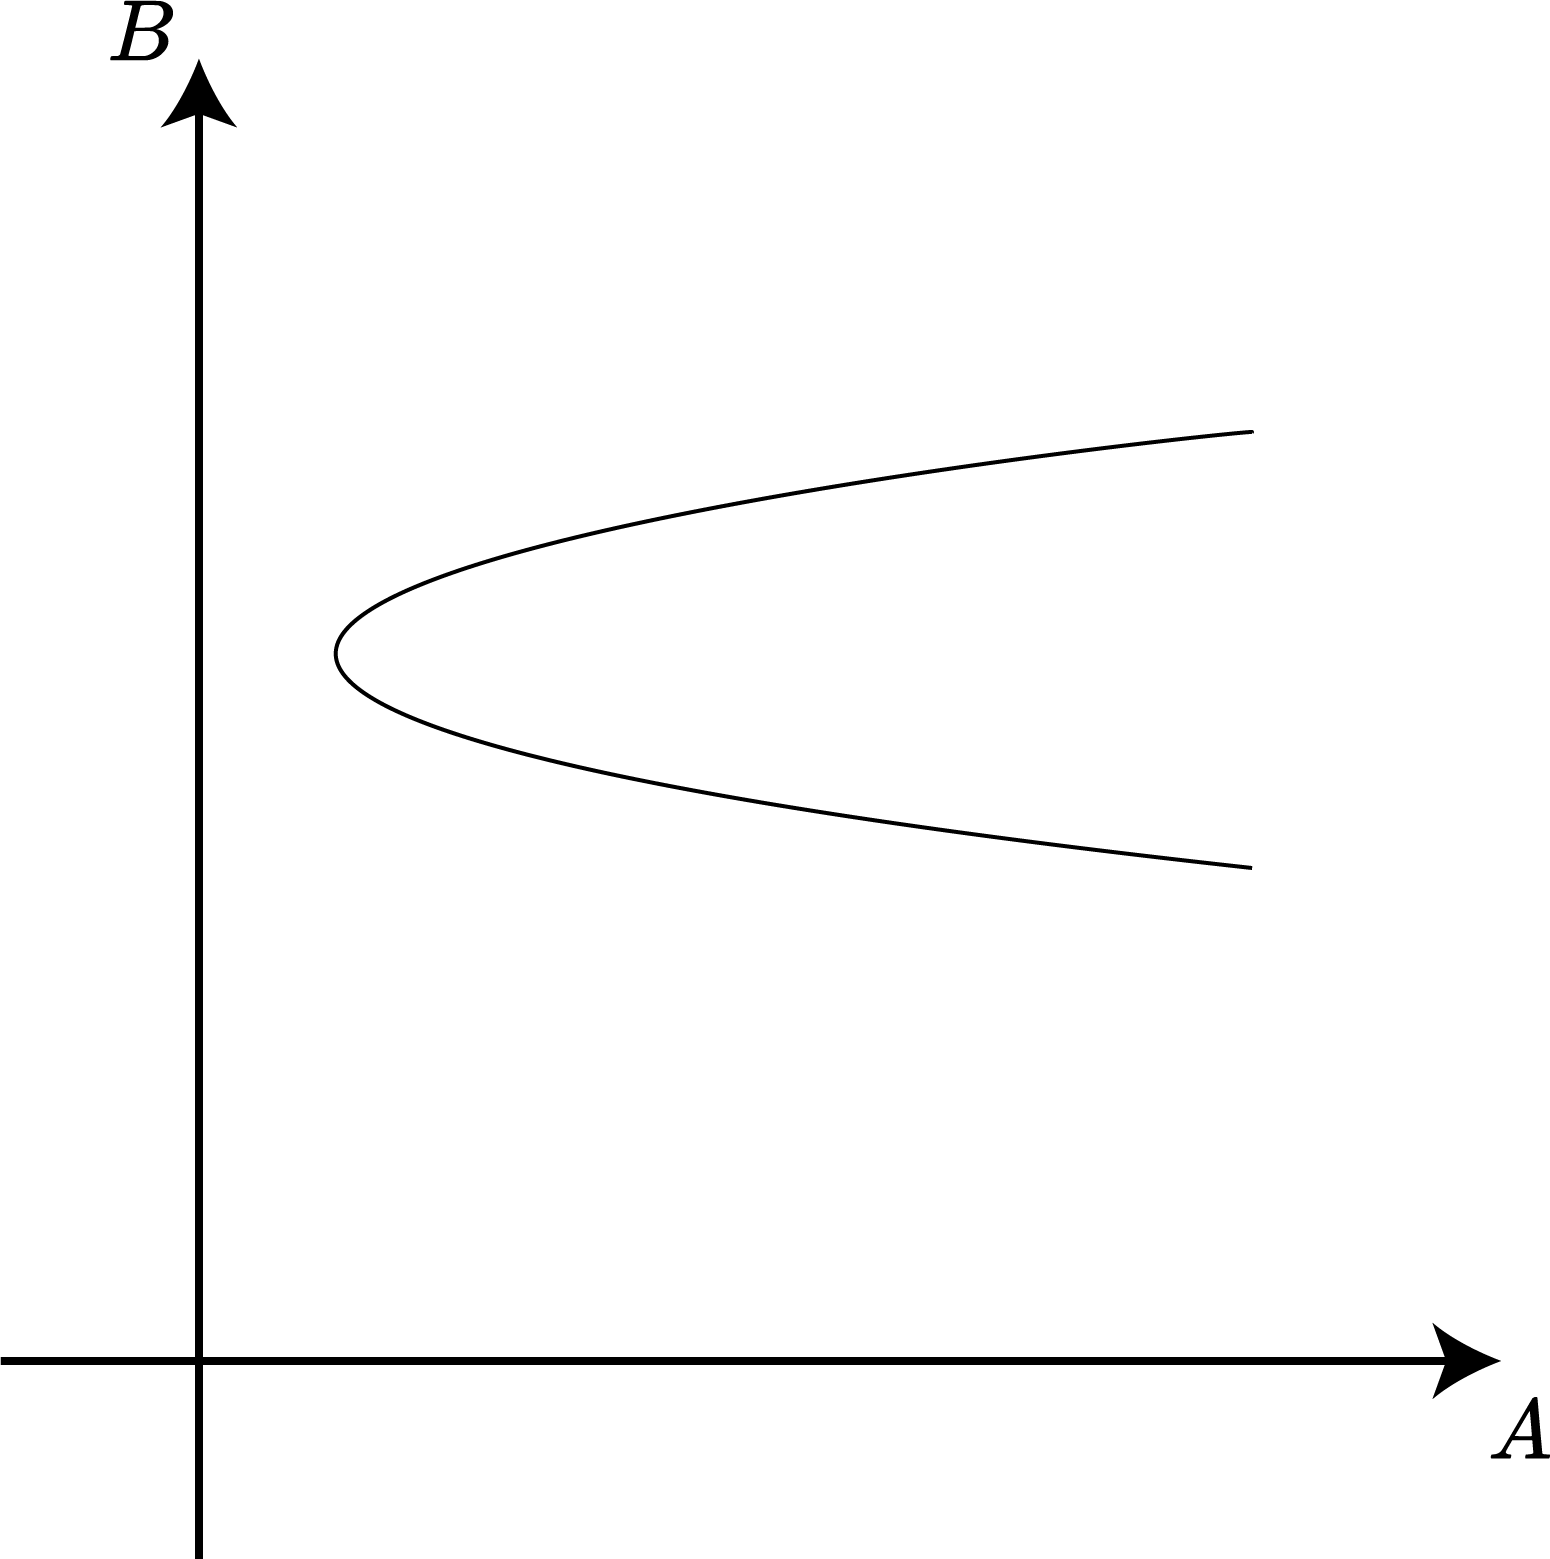
\includegraphics[width=0.3\textwidth]{images/img06.png}\\
	$P\subset A\times B$ ist der Graph einer Funktion genau dann, wenn aus $(a_1,b_1), (a_2,b_2) \in \Gamma$ folgt $b_1 = b_2$. (und $\forall a\in A \exists b\in B:(a,b)\in\Gamma$)
\end{defi}
\begin{satz}
	$\Gamma \subset A\times B$ ist genau dann Graph einer Abbildung $f: A\rightarrow B$, wenn die Projektion $\Pi_A \vert_\Gamma : \Gamma \rightarrow A$ bijektiv ist.\\
	Notation: $g: D \rightarrow E, X\subset D$\\
	$g\vert_X: X\rightarrow E, x\mapsto g(x)$\\
\end{satz}
\begin{bew}
	Sei $\Gamma = \Gamma_f$ mit $f: A\rightarrow B$ Funktion\\
	$\overset{(a,b)\in \Gamma_f \Leftrightarrow b = f(a)}{\Rightarrow} \forall a\in A$ existiert genau ein $b\in B$ mit $f(a) = b$.\\
	$\Rightarrow \Pi_A \vert_\Gamma$ ist bijektiv.\\
	Umgekehrt: Sei $\Pi_A \vert_\Gamma \rightarrow A$ bijektiv.\\
	D.h. ist $(a_j, b_j) \in \Gamma, j \in\{1,2\}$\\
	und $\Pi_A(a_1, b_1) = \Pi_A(a_2, b_2) \Rightarrow (a_1, b_1) = (a_2, b_2)$\\
	$\Leftrightarrow a_1 = a_2, b_1 = b_2$\\
	$\Rightarrow$ zu $a\in A \exists ! b\in B, (a,b) \in \Gamma$.\\
	Da $b=\Pi_B(a,b) = \Pi_B((\Pi_A\vert_\Gamma)^{-1}(a))$\\
	Definiere $f:= \Pi_B \circ (\Pi_A\vert_\Gamma)^{-1}:A\rightarrow B$ ist Funktion\\
	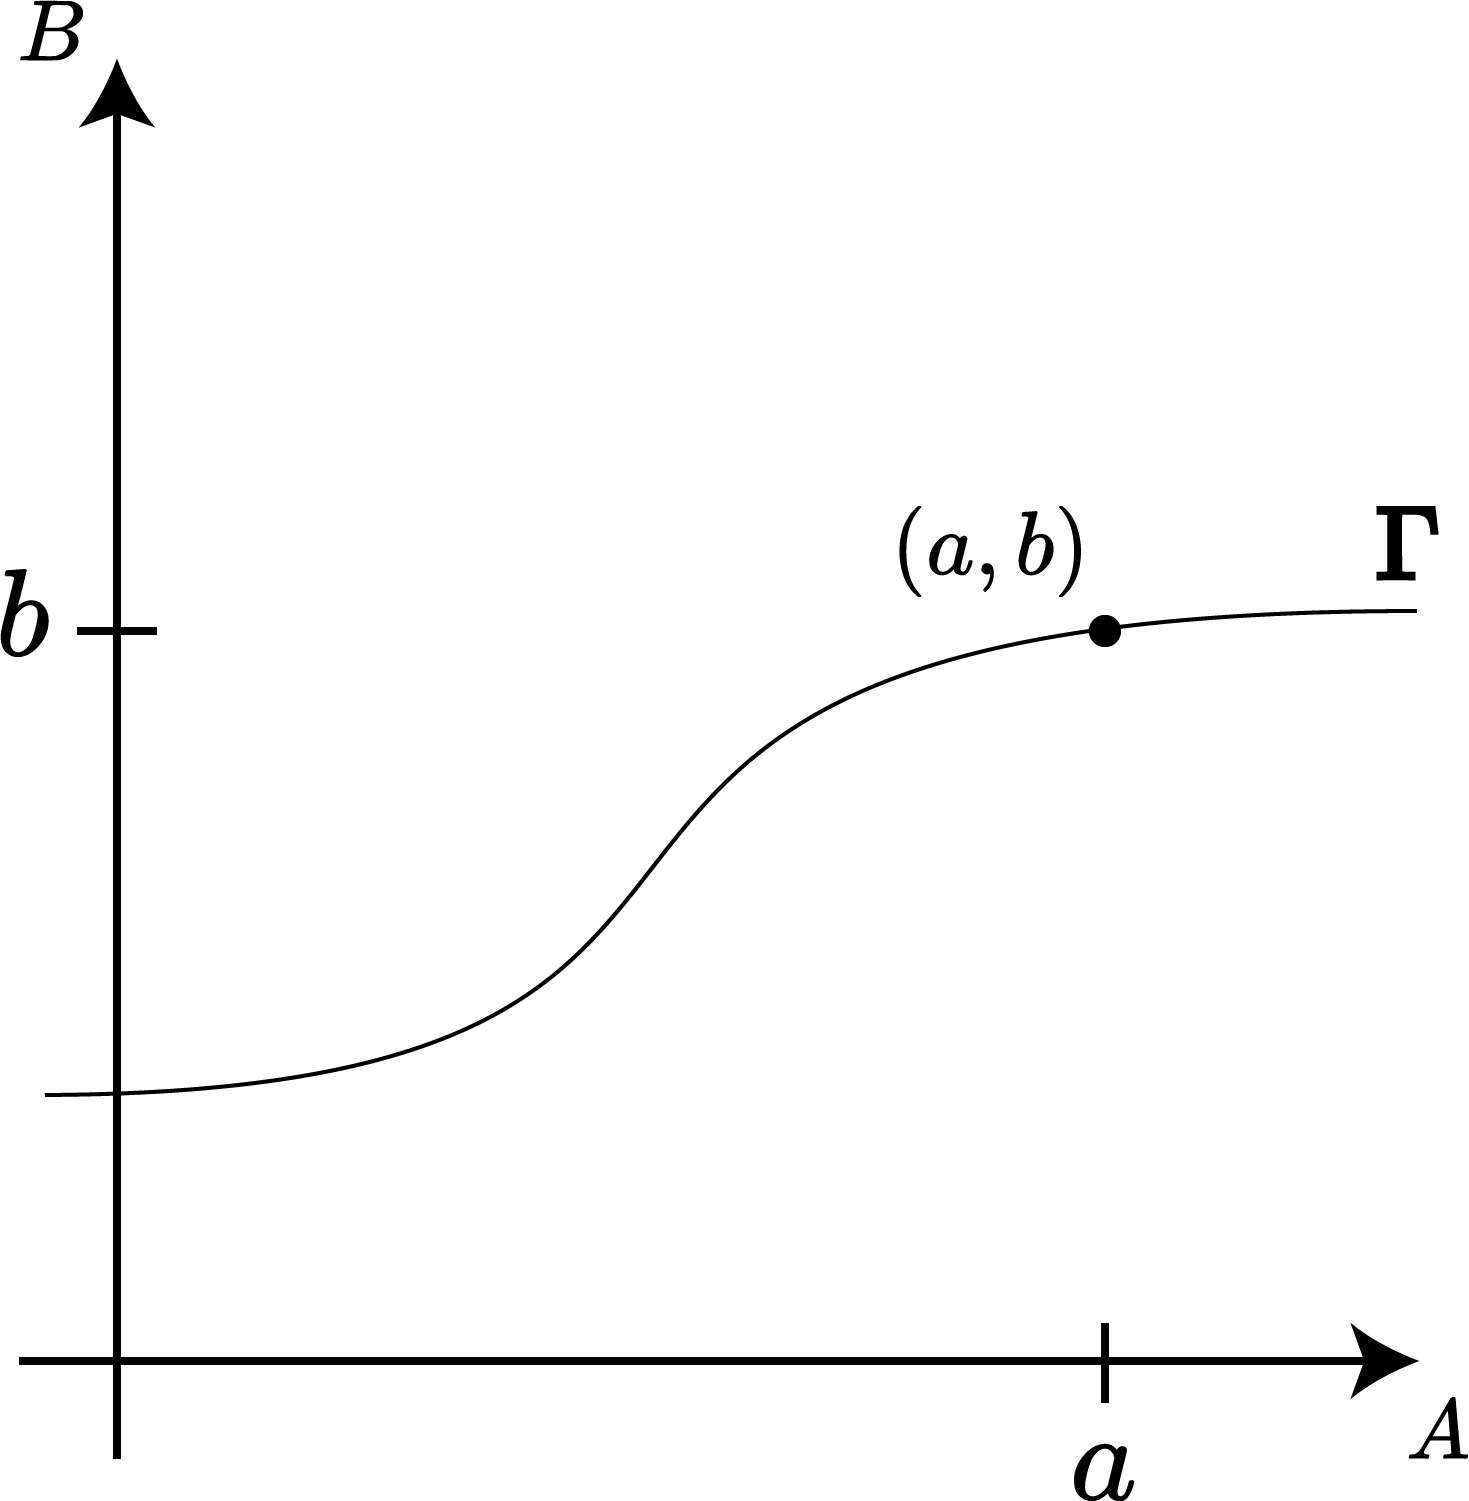
\includegraphics[width=0.3\textwidth]{images/img07.png}\\
	nachrechnen $\Gamma = \Gamma_f$
\end{bew}
\begin{bem}
	In Satz 3 gilt $f = \Pi_B \circ (\Pi_A\vert_\Gamma)^{-1}$ %ENTSPRICHT 4.2
\end{bem}
\begin{bsp}
	Ist $f: A\rightarrow B$ bijektiv\\
	$b=f(a),\quad f^{-1}(b)=a$\\
	Dann gilt: $\Gamma_f^{-1} = \{(b, f^{-1}(b)) | b\in B\}\\
	= \{(f(a),a):a\in A\} = S(\Gamma_f), S: A\times B \rightarrow B\times A$ (swap), $(a,b)\mapsto(b,a)$.\\
	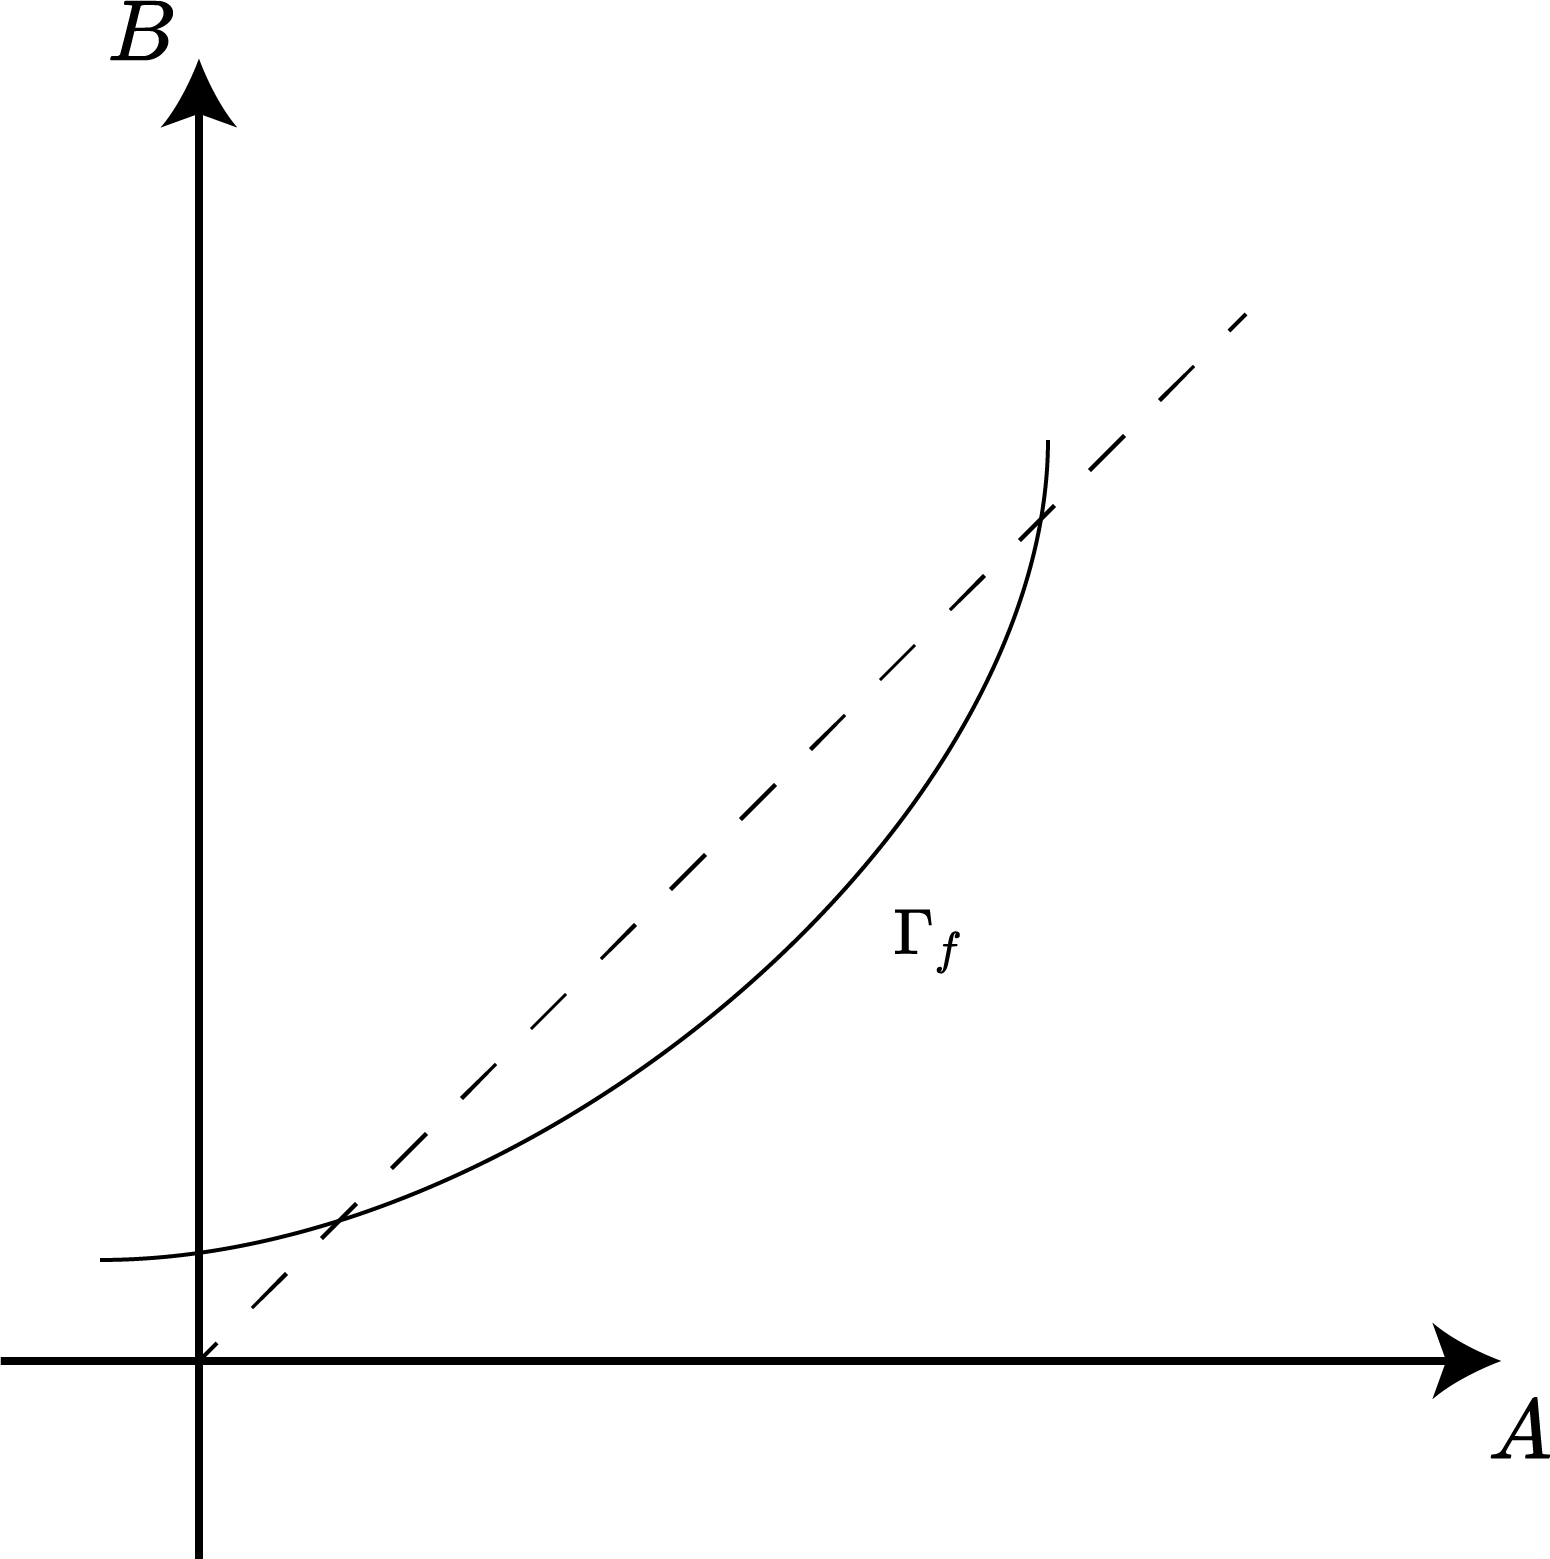
\includegraphics[width=0.3\textwidth]{images/img08.png} \quad
	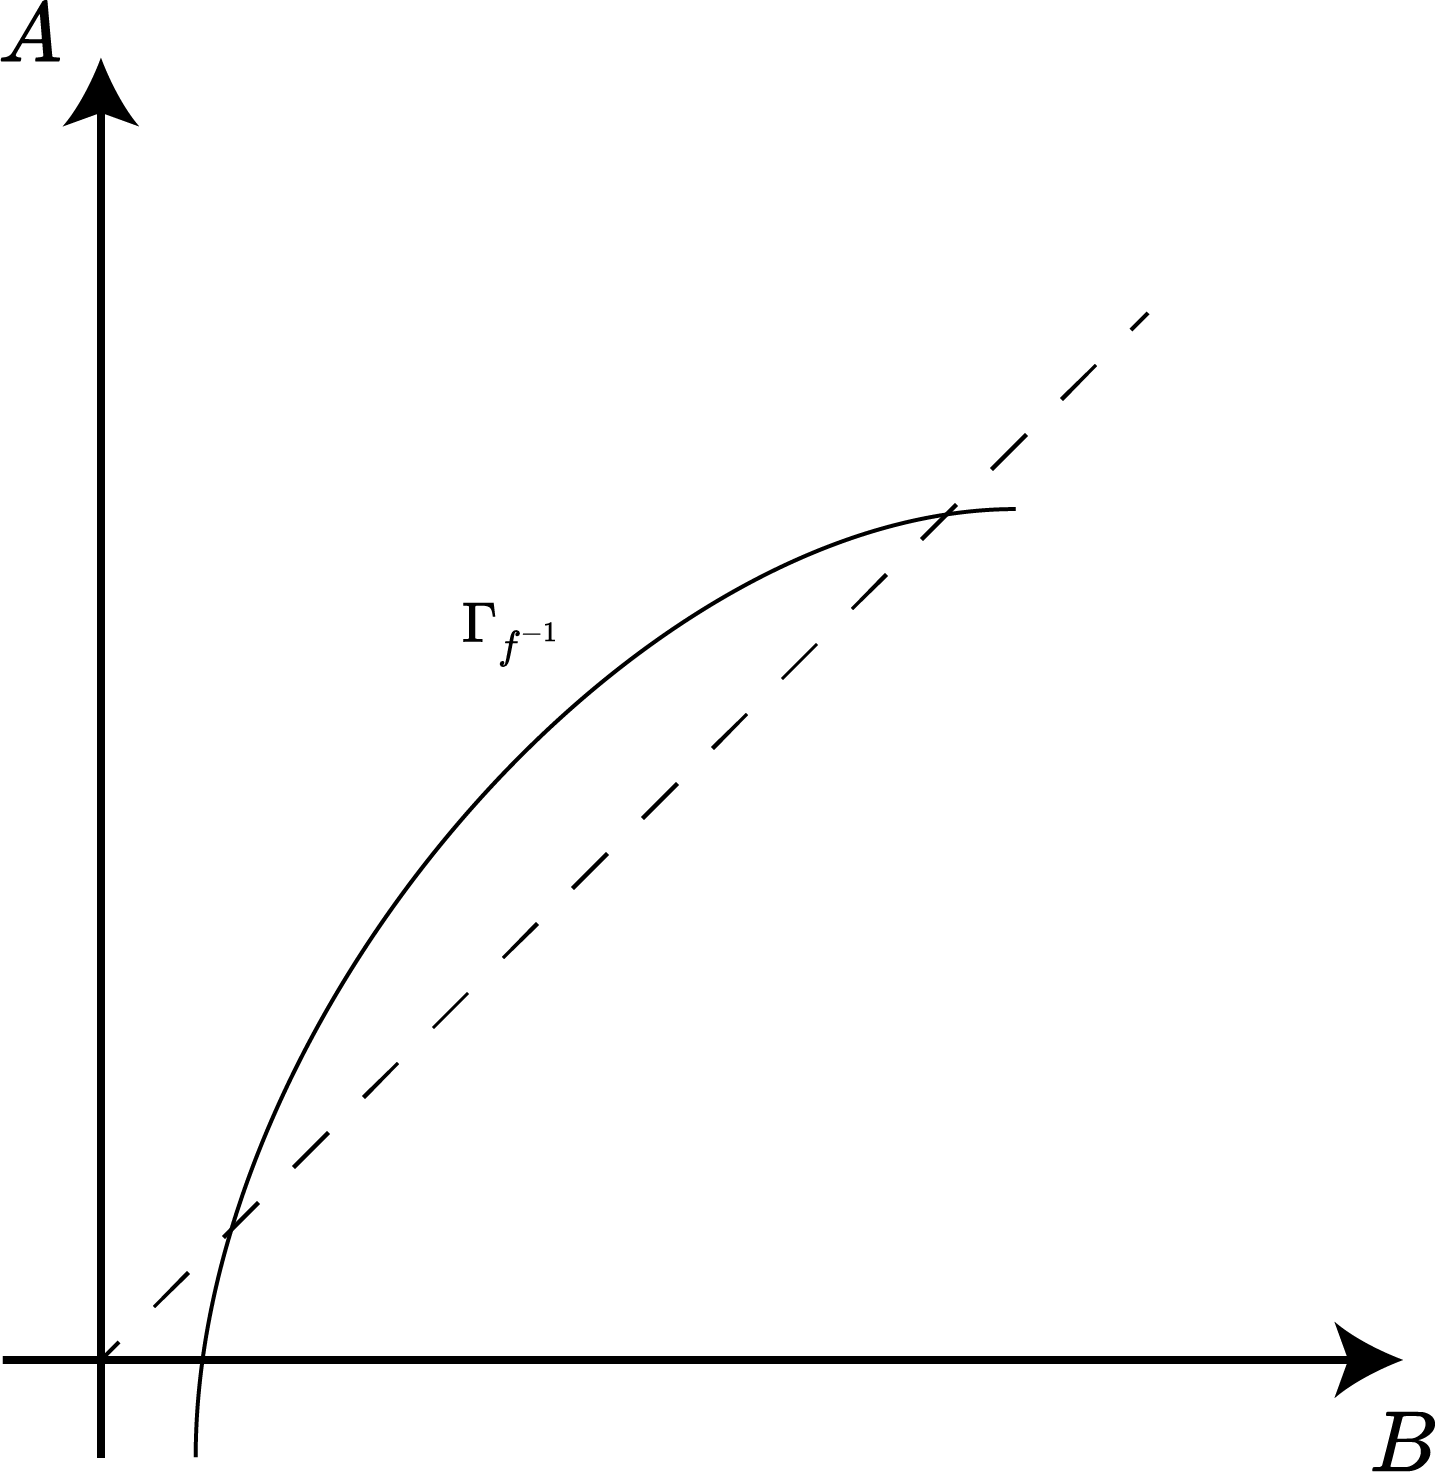
\includegraphics[width=0.3\textwidth]{images/img09.png}\\
	$\Gamma_{f^{-1}} = $ Spiegeln von $\Gamma_f$ an Winkelhalbierenden.
\end{bsp}
\subsection{Schubfachprinzip und endliche Mengen}
Notation: Sei $n\in\mathbb{N}. [n] := \{1,\ldots,n\}$ ist gegeben durch:
$$[1] = \{1,\ldots,1\} = \{1\}$$
$$[n+1] = \{1,\ldots,n,n+1\} = [n] \cup \{n+1\}\text{ induktive Def.} n\in\mathbb{N}$$
$$[2]=\{1,2\}, [3]=\{1,2,3\}$$
\begin{satz}[Schubfachprinzip]
	Ist $f:[m]\rightarrow [n] (m,n\in\mathbb{N})$ injektiv, dann ist $m\leq n$.
\end{satz}
\begin{bew}
	Fassen obige Aussage als $A(n)$ auf, die für alle $m\in\mathbb{N}$ zu zeigen ist.\\
	Induktionsanfang: $$n=1: f:[m] \rightarrow \{1\} \text{ injektiv} \Rightarrow m=1, \text{ da sonst } f(1) = 1 = f(2) \text{\Lightning zu Injektivität}.$$
	Induktionsschritt:\\
	Induktionsvoraussetzung: $A(n)$ ist wahr für $n\in\mathbb{N}$.\\
	Zu zeigen: $A(n+1)$ ist wahr.\\
	Angenommen, $f:[m]\rightarrow[n+1] = [n] \cup \{n+1\}$ sei injektiv.\\
	Zu zeigen: $m\leq n+1$\\
	Fallunterscheidung:
	\begin{enumerate}
		\item Ang. $m=1 \Rightarrow m=1\leq n+1\checkmark$
		\item Ang. $m>1, m\in\mathbb{N} \overset{\text{Satz 3.5.8}}{\Rightarrow} m-1\in\mathbb{N}$\\
		$(*)$ Beh.: $\exists$ inj. $\tilde{f}: \{1,\ldots,m-1\}\rightarrow\{1,\ldots,n\}$.\\
		$$\overset{(*) + \text{IV}}{\Rightarrow} m-1\leq n, \text{ d.h. } m\leq n+1 \Rightarrow A(n+1) \text{ ist wahr}.$$		
	\end{enumerate}
	Beweis von $(*)$:\\
	Angenommen, $\exists f: [m]\rightarrow[n+1]$ inj.\\
	Dann $\exists \tilde{f}: [m+1]\rightarrow [m+1]\rightarrow[n]$ inj.\\
	Fallunterscheidung:
	\begin{itemize}
		\item Ang. $f(k)\in [n] \forall 1\leq k \leq m-1$. Dann setze $\tilde{f}(k) := f\vert_{[m-1]}\\
		\tilde{f}(k) := f(k), 1\leq k\leq m-1$\\
		(Nachrechnen $\tilde{f}$ ist injektiv.)
		\item $\exists j\in\mathbb{N}, 1\leq j\leq m-1$ mit $f(j) = n+1$.\\
		Dann def. $\tilde{f}: [m-1]\rightarrow [n]$
		$$\tilde{f}(k) :=
		\begin{cases}
			f(k), 1 \leq k \leq m-1, k\neq j\\
			f(m), k=j
		\end{cases}$$
		Man prüfe nach $\tilde{f}: [m-1]\rightarrow [n]$ injektiv!
	\end{itemize}
\end{bew}
\begin{kor}
	Sind $n,m\in\mathbb{N}$ und $f:[m]\rightarrow[n]$ bijektiv $\Rightarrow m=n$.
\end{kor}
\begin{bew}
	Nach Voraussetzung ist $f: [m]\rightarrow[n]$ injektiv und $f^{-1}:[n]\rightarrow[m]$ auch injektiv.\\
	$\Rightarrow m\leq n \wedge n \leq m \Rightarrow m = n$.
\end{bew}
\begin{defi}
	Eine Menge $M$ ist \underline{endlich}, falls $M=\emptyset$ oder falls $n\in\mathbb{N}_0$ und eine Bijektion $f:{1,\ldots,n}\rightarrow M$ existiert.\\
	Die Anzahl der Elemente von $M$ ($\#M$) ist dann $\#M:=n$, setzen $\#\emptyset := 0$. Eine Menge ist unendlich, falls sie nicht endlich ist.
	\begin{bem}
		Ist $M$ endlich, so ist $\#M$ wohldefiniert. \\
		Angenommen: 
		$$\begin{array}{lr}
		f:[n]\rightarrow M\\
		g:[m]\rightarrow M
		\end{array}
		\text{ beide bijektiv.}$$
		$$[n]\overset{f}{\longrightarrow} M \overset{g}{\longleftarrow} [m]$$
		$h:= f^{-1}\circ g = [m]\rightarrow[n]$ ist auch bijektiv. $\overset{\text{Korr. 2}}{\Rightarrow} m=n.$
	\end{bem}
	Weiter in Definition:\\
	Zwei Mengen $A,B$ heißen \underline{gleichmächtig}, falls es eine Bijektion $f: A\rightarrow B$ gibt, schreiben $A\sim B$. Eine Menge $A$ heißt \underline{abzählbar}, falls $A$ endlich ist oder es eine Bijektion $f: \mathbb{N}\rightarrow A$ gibt. Ist $A$ abzählbar und unendlich, so heißt $A$ abzählbar unendlich.
\end{defi}
\begin{bem}
	Satz von Cantor und Berenstein:\\
	Ang. $\exists$ Injektion $f:A\rightarrow B, f:B\rightarrow A$, dann $\exists$ Bijektion $h:A\rightarrow B$.
\end{bem}
\begin{bew}
	Siehe Kolmogorov-Fomin: Introductory Real Analysis.\\
	Könnten definieren $A\leq B$, falls es eine inj. Funktion $f: A\rightarrow B$ gibt.\\
	$A\leq B \wedge B\leq A \Leftrightarrow A\sim B$.
\end{bew}
\begin{bem}
	$A\leq B$ heißt Kardinalität von $A$ ist kleiner gleich der Kardinalität von $B$.
	\begin{enumerate}
		\item Ist $B\subset A$ und $A$ endlich, so ist $B$ endlich und $\#B \leq \# A$.
		\item $A,B$ endlich und disjunkt, $A\cap B = \emptyset \Rightarrow \#(A\cup B) = \#A + \#B$.
	\end{enumerate}
\end{bem}
\begin{satz}
	\begin{enumerate} . %SCHLECHT FORMATIERT
		\item Jede Teilmenge einer abzählbaren Menge ist abzählbar.
		\item Sind für $j\in\N \quad A_j$ abzählbare Mengen. Dann ist $\bigcup_{j\in\N}$ abzählbar.
	\end{enumerate}
\end{satz}
\begin{bew} . % SCHLECHT FORMATIERT
	\begin{enumerate}
		\item Sei $A$ abzählbar. Ist $A$ endlich, so ist auch jedes $B\subset A$ endlich, und somit abzählbar.\\
		Sei $A$ abzählbar unendlich. Dann existiert eine Bijektion $f: \N \rightarrow A$ und setzen wir $a_n := f(n)$, so ist
		$$A = \bigcup_{n\in\N} \{a_n\} = \{a_1, a_2,\ldots\}.$$
		Ist $B\subset A$, so existieren $n_j \in\N, 1\leq n_1<n_2<\ldots$ mit $$B = \{a_{n_1}, a_{n_2}, \ldots\}.$$
		Gibt es nur endlich viele $n_j$, so ist $B$ endlich, andernfalls ist $h: \N \rightarrow B, g \mapsto h(j) := a_{n_j}$
		eine Bijektion.
		\item o.B.d.A. sind alle $A_j$ paarweise verschieden, $A_l \cap A_m \neq \emptyset$ für \(l\neq m\).
		Wenn nicht, betrachte 
		\[B_1 := A_1, \quad B_2 := A_2 \setminus A_1,\]
		\[B_3 := A_3 \setminus \{A_1 \cup A_2\}, \ldots, \quad B_{n+1} := A_{n+1} \setminus \{A_1\cup\ldots\cup A_n\}\]
		Dann sind \(B_n\) paarweise verschieden und \[\bigcup_{l\in\N} B_l = \bigcup_{l\in\N} A_l.\]
		Schreiben \(A_l\) als Liste \(A_l = \{a_{1l}, a_{2l}, \ldots\}\)\\
		Bild: 
		\begin{tikzpicture}
		\matrix(m)[matrix of math nodes,column sep=1cm,row sep=1cm]{
			s_{11} & s_{12} & s_{13} & s_{14} & \cdots \\
			s_{21} & s_{22} & s_{23} & s_{24} & \cdots \\
			s_{31} & s_{32} & s_{33} & s_{34} & \cdots \\
			s_{41} & s_{42} & s_{43} & \cdots \\
		};
		
		\draw[->]
		(m-1-1)edge(m-1-2)
		(m-1-2)edge(m-2-1)
		(m-2-1)edge(m-3-1)
		(m-3-1)edge(m-2-2)
		(m-2-2)edge(m-1-3)
		(m-1-3)edge(m-1-4)
		(m-1-4)edge(m-2-3)
		(m-2-3)edge(m-3-2)
		(m-3-2)edge(m-4-1);
		\end{tikzpicture}
		Jetzt können wir das obige rechteckige Schema diagonal abzählen! Dies liefert uns eine Bijektion von \(\N\) nach \(\bigcup_l\in\N A_l\).
	\end{enumerate}
\end{bew}
\begin{bem}
	Als Übung: Man gebe explizit eine Bijektion \(f : \N \rightarrow \N \times \N\) an!
\end{bem}
\textbf{Permutationen:}
\begin{defi}
	Eine bijektive Abbildung \(\sigma : \{1,\ldots,n\} \rightarrow \{1,\ldots,n\}\) heißt \underline{Permutation}.
	\[n! = \prod_{k=1}^{n}k\]
\end{defi}
\begin{satz}
	\[n\in\N, S_n = \{\sigma: \{1,\ldots,n\}\rightarrow\{1,\ldots,n\} | \sigma \text{ ist bijektiv.}\} \Rightarrow \# S_n = n!\]
\end{satz}
\begin{bew} per Induktion\\
	\(n = 1\) ist klar.
	Beobachtung: Permutation \(\sigma \in S_n\) identifizieren mit \(n\)-Tupel \( (\sigma(1), \sigma(2), \ldots, \sigma(n))\)\\
	Induktionsannahme: \(\# S_n = n!\) für ein \(n\in\N\)\\
	Die Menge \(S_{n+1}\) ist die disjunkte Vereinigung der Teilmengen 
	\[S_{n+1, k} := \{\tau \in S_{n+1} | \tau_k = n+1 \} \quad k = 1,\ldots, n+1.\]
	z.B.: \[S_{4,2} = \{ (1,4,2,3), (2,4,3,1), (3,4,1,2), (1,4,3,2), (2,4,1,3), (3,4,1,2) \}\]
	Beobachtung: Jedem \(\tau = (\sigma_1,\ldots,\sigma_n)\in S_n\) können wir die Permutation \( (\sigma_1, \ldots, \sigma_{k-1}, \underbrace{n+1}_{k\text{-te Stelle}}, \sigma_k, \ldots, \sigma_n) \in S_{n,k} \) zuordnen \underline{und} diese Abbildung ist \underline{bijektiv} (nachprüfen).
	\[\Rightarrow \# S_{n+1,k} = \# S_n \]
	\[ S_{n+1} = \# (\bigcup_{k=1}^{n+1} S_{n+1,k} ) = \sum_{k=1}^{n+1} \underbrace{\# S_{n+1,k}}_{=\#S_n = n!} = \sum_{k=1}^{n+1} n! = (n+1)n! = (n+1)! \]
\end{bew}
\begin{defi}[Binomialkoeffizient]
	Für \(\alpha \in\R \) und \( k\in\N \) setzen wir
	\[ \binom{\alpha}{k} := \frac{\alpha(\alpha-1)\cdot\ldots\cdot(\alpha-k+1)}{k!}, \text{ sowie } \binom{\alpha}{0} := 1. \]
\end{defi}
\begin{lem}[Rekursionsformel für Binomialkoeffizienten]
	Für \( \alpha\in\R, k\in\N \) gilt \[ \binom{\alpha + 1}{k} = \binom{\alpha}{k} + \binom{\alpha}{k-1}. \]
\end{lem}
\begin{bew}
	Für \(k=1\) ist dies einfach zu sehen. Für \(k\geq 2\) gilt 
	\begin{align*}
		&\binom{\alpha}{k} + \binom{\alpha}{k-1} \\
		&= \frac{\alpha (\alpha-1)\cdot\ldots\cdot(\alpha-k+1)}{1\cdot2\cdot\ldots\cdot k} + \frac{\alpha (\alpha-1)\cdot\ldots\cdot(\alpha-k+2)}{1\cdot2\cdot\ldots\cdot (k-1)}\\
		&= \frac{\alpha (\alpha-1)\cdot\ldots\cdot(\alpha-k+2)(\alpha-k+1+k)}{1\cdot2\cdot\ldots\cdot k}\\
		&= \frac{(\alpha + 1)\alpha (\alpha-1)\cdot\ldots\cdot((\alpha-1)-k+1)}{1\cdot2\cdot\ldots\cdot k} = \binom{\alpha + 1}{k}
	\end{align*}
\end{bew}
\begin{bem}
	\begin{enumerate}.%SCHLECHT FORMATIERT
		\item Ist \(\alpha = n\in\N_0\), so können wir \(\binom{n}{k}\) ausrechnen mit dem Dreiecksschema von Blaise Pascal (1623-1662).\\
		\begin{tabular}{>{$n=}l<{$\hspace{12pt}}*{13}{c}}
			0 &&&&&&&1&&&&&&\\
			1 &&&&&&1&&1&&&&&\\
			2 &&&&&1&&2&&1&&&&\\
			3 &&&&1&&3&&3&&1&&&\\
			4 &&&1&&4&&6&&4&&1&&\\
			5 &&1&&5&&10&&10&&5&&1&\\
			6 &1&&6&&15&&20&&15&&6&&1
		\end{tabular}
		\item Ist \( \alpha=n\in\N_0 \), so folgt durch Erweitern mit \((n-k)!\) für \(n \in\N_0, k\in\{0,1,\ldots,n\} \) \[ \binom{n}{k} = \frac{n!}{k!(n-k)!} = \binom{n}{n-k}. \]
	\end{enumerate}
\end{bem}
\begin{satz}[Zahl der Kombinationen]
	Sei \( n\in\N_0, k\in\{1,\ldots,n\} \). Dann ist die Anzahl der \(k\)-elementigen Teilmengen von \( \{1,\ldots,n\} \) gleich \( \binom{n}{k} \).
\end{satz}
\begin{bew}
	Die Behauptung gilt für \(k=0\) und beliebiges \(n\in\N\), da die leere Menge die einzige Teilmenge von \( \{1,\ldots,n\} \) mit 0 Elementen ist und nach Def. ist \( \binom{n}{0} = 1 \).\\
	Insbesondere gilt die Behauptung dann für \(n=0\).\\
	Induktiv über \(n\), wobei Behauptung für alle \(k\in\{0,1,\ldots,n\}\) zu zeigen ist.\\
	Induktionsschluss: Bestimme die Anzahl der \(k\)-elementigen Teilmengen von \(\{ 1,\ldots,n+1 \}\) (wobei wir \(k\geq 1\) annehmen können).\\
	Sei \(A\subset \{1,\ldots,n+1\}\) mit \(\#A = k\geq 1\). \\
	Diese fallen in 2 Klassen:
	Klasse 1: \(n+1 \notin A\).\\
	Klasse 2: \(n+1 \in A\).\\
	Die Mengen der Klasse 1 bestehen genau aus den \(k\)-elementigen Teilmengen von \(\{1,\ldots,n\}\).\\
	Die Mengen der 2. Klasse erhält man aus den \((k-1)\)-elementigen Teilmengen von \(\{1,\ldots,n\}\) durch Vereinigung mit \(\{n+1\}\).\\
	Also ist nach Induktionsannahme
	\begin{align*}
		&\#\{k\text{-elementige Teilmengen von } \{1,\ldots,n+1\} \}\\
		&=\#\{k\text{-elementige Teilmengen von } \{1,\ldots,n\} \} \\&+ \#\{(k-1)\text{-elementige Teilmengen von } \{1,\ldots,n\} \} \\
		&\overset{\text{IV}}{=} \binom{n}{k} + \binom{n}{k-1} \overset{\text{Lem. 8}}{=} \binom{n+1}{k}.
	\end{align*}
\end{bew}
\begin{satz}[Binomische Formel]
	\[ a,b\in\R,n\in\N:(a+b)^n = \sum_{k=0}^{n} \binom{n}{k} a^k b^{n-k}. \]
\end{satz}
\begin{bem}
	\begin{align}
		(a+b)^1 &= a+b\\
		(a+b)^2 &= a^2 + 2ab + b^2\\
		(a+b)^3 &= a^3 +3a^2b + 3ab^2 +b^3
	\end{align}
\end{bem}
\begin{bew} Induktion
	\[n=1: (a+b)^1 = a+b = \sum_{k=0}^{1}\binom{1}{k} a^kb^{1-k} \checkmark \]
	Induktionsvoraussetzung: für ein beliebiges, aber festes \(n \in\N\) gilt: 
	\[(a+b)^n = \sum_{k=0}^{n} \binom{n}{k} a^kb^{n-k}. \]
	Induktionsschritt: 
	\begin{align*}
		(a+b)^{n+1} &= (a+b) (a+b)^n = (a+b) \sum_{k=0}^{n} \binom{n}{k} a^kb^{n-k}\\
		&= \sum_{k=1}^{n+1} \binom{n}{k-1} a^kb^{n-(k-1)} + \sum_{k=0}^{n} \binom{n}{k} a^kb^{n+1-k}\\
		&= \binom{n}{n} a^{n+1} + \sum_{k=1}^{n} \binom{n}{k-1} a^kb^{n+1-k} + \sum_{k=1}^{n} \binom{n}{k} a^kb^{n+1-k} + \binom{n}{0} b^{n+1}\\
		&= \binom{n+1}{n+1} a^{n+1} + \sum_{k=1}^{n} \underbrace{\left(\binom{n}{k-1} + \binom{n}{k}\right)}_{=\binom{n+1}{k}} a^kb^{n+1-k} + \binom{n+1}{0} b^{n+1}\\
		&= \sum_{k=0}^{n+1} \binom{n+1}{k} a^kb^{n+1-k}\\
		&= \sum_{k=0}^{n+1} \binom{n+1}{k} a^kb^{n+1-k}.
	\end{align*}
\end{bew}
\textbf{Notation:} Geg. Menge \(A\), sei \[ \{0,1\}^A := \{ \text{Funktion }f:A\rightarrow \{0,1\} \} \] \(= \) Menge aller \(\{0,1\}\)-wertigen Funktionen mit Definitionsbereich \(A\).\\
Allg.: \(A,B\) Mengen, \(B^A := \{ \text{Funktion } f: a\rightarrow B\}\).
\begin{satz}
	Sei \(A\neq\emptyset\) eine endliche Menge. Dann ist \[\#(\{0,1\}^A) = 2^{\#A}.\]
\end{satz}
\begin{bew}
	Sei \(n := \# A \in\N \).\\
	\(\Rightarrow\) Bijektion \(h:\{1,\ldots,n\} \rightarrow A\).\\
	\( \Rightarrow \) können annehmen \(A = \{1,2,\ldots,n\}\)\\
	z.z. \(\#( \{0,1\}^[n] ) = 2^n\).\\
	Induktion: \(n=1 \exists \) Fkt. \(f_1,f_2 : \{1\} \rightarrow \{0,1\} \\
	f_1(1) = 0 \quad f_2(1) = 1 \)\\
	Formel stimmt für \(n=1\).
	Ang. Formel stimmt für \(n\geq 1\). Fkt. \(f: \{1,\ldots, n+1\} \rightarrow \{0,1\} \)\\
	2 Klassen: 
	\begin{enumerate}
		\item \(S_0 = \{f: \{1,\ldots,n\} \rightarrow \{0,1\}: f(n+1) = 0 \}\)
		\item \(S_1 = \{f: \{1,\ldots,n\} \rightarrow \{0,1\}: f(n+1) = 1 \}\)
	\end{enumerate}
	\[S_0 \cap S_1 = \emptyset, \{0,1\}^{[n+1]} = S_0 \cup S_1 \]
	\[\underbrace{\# S_0}_{=\#S_1} = \# (\{0,1\}^{[n]})  \overset{\text{IA}}{=} 2^n \]
	\[ \Rightarrow \# (\{0,1\}^{n+1}) = \#S_0+\#S_1 = 2^n + 2^n = 2^{n+1}. \]
\end{bew}
\begin{kor}
	Sei \(A\) endliche Menge. \\
	\(\mathcal{P}(A) = \) Potenzmenge = \(\{B | B \subseteq A\}\)\\
	\(\Rightarrow \#\mathcal{P}(A = 2^{\#A}) \).
\end{kor}
\begin{bew}
	Sei \(A\neq \emptyset \Rightarrow\mathcal{P}(\emptyset) = \{\emptyset\}, \quad 2^0 = 1 \checkmark \)\\
	Sei \(\#A \in\N\). Nach Satz 11 reicht eine Bijektion \( \varphi : \mathcal{P} \rightarrow \underbrace{\{0,1\}^A}_{= \{f: A \rightarrow \{0,1 \} \}} \). Dies wird in Lemma 13 für bel. Mengen \(A\) gemacht.
\end{bew}
\begin{lem}
	Sei \(A\neq\emptyset\). Dann sind \( \mathcal{P}(A) \) und \(\{0,1\}^A\) gleichmächtig.
\end{lem}
\begin{bew}
	Brauchen \(\varphi : \mathcal{P}(A) \rightarrow \{0,1\}^A \).\\
	Sei \(B \subseteq A \), Indikatorfunktion \[ \mathds{1}_B(x) := \begin{cases} 
	1, &x\in B\\
	0, &x\in A\setminus B
	\end{cases}
	, \mathds{1}_B : A \rightarrow \{0,1\}. \]
	Beachte: \(B = \{x\in A | \mathds{1}_B(x) = 1 \} \).\\
	Definiere \( \varphi : \mathcal{P}(A) \rightarrow \{0,1\}^A, B \mapsto \mathds{1}_B \).\\
	Beh.: \(\varphi\) ist bijektiv.
	\begin{enumerate}
		\item \( \varphi \) ist surjektiv.\\
		Sei \(f: A\rightarrow \{0,1\}\)
		\[ B_f := f^{-1} (\{1\}) = \{a \in A| f(a) = 1 \} \Rightarrow \varphi(B_f) = \mathds{1}_{B_f} = f\text{ (nachrechnen)}.\]
		\item \( \varphi \) ist injektiv.\\
		Seien \( B_1,B_2\subseteq A, B_1 \neq B_2 \).
		\begin{align*}
			B_1\setminus B_2 \neq \emptyset \vee B_2\setminus B_1 \neq \emptyset\\
			\text{o.B.d.A. } B_1 \setminus B_2 \neq \emptyset \Rightarrow \exists x \in B_2 \setminus B_1 \subset A\\
			\mathds{1}_{B_1}(x) = 0 \neq 1 = \mathds{1}_{B_2}(x)\\
			\Rightarrow \varphi(B_1) = \mathds{1}_{B_1} \neq \mathds{1}_{B_2} = \varphi(B_2).
		\end{align*}
	\end{enumerate}
\end{bew}
\begin{lem}
	Sei \(A\) Menge. Dann gibt es keine surj. Fkt. \(f: A\rightarrow \mathcal{P}(A) \).
\end{lem}
\begin{bem}
	Ist \(A\) endlich \( \Rightarrow \# \mathcal{P} (A) = 2^{\# A} > \#A \).\\
	\( \varphi: \mathcal{P}(A) \rightarrow \{0,1\}^A, \quad A\supset B \mapsto \mathds{1}_B \).
\end{bem}
\begin{bew}
	Sei \(f: A \rightarrow \mathcal{P}(A) \)
	\[ f(A) \subset A \quad \forall a \in A. \]
	Definiere \(R := \{a\in A, a \neq f(a)\} \subset A \).\\
	Angenommen \(f: A \rightarrow \mathcal{P}(A) \) ist surjektiv.
	\[ \Rightarrow \forall b\in A \exists b : B=f(b) \Rightarrow \exists a\in A : R = f(a). \]
	\(\Rightarrow\) 2 Möglichkeiten:
	\begin{enumerate}
		\item \(a\in R\) \[ a\in f(a = R = \{x\in A| x\notin f(x)\}) \text{\Lightning} \]
		\item \(a \notin R = f(a) \Rightarrow a \notin f(a) \Rightarrow a\in R \) \Lightning\\
		\( f\) kann nicht surjektiv sein!
	\end{enumerate}
\end{bew}

%FERTIG MACHEN

\newpage
%09.11.2018
\section{}
\subsection{Starke Induktion und das Wohlordnungsprinzip}
\begin{satz}[starke Induktion]
	Seien $A(n)$ Aussagen für $n\in\mathbb{N}$. Dann gilt
	\begin{enumerate}
		\item $A(1)$ ist wahr
		\item $\forall n\in\mathbb{N}: A(1), \ldots, A(n)$ wahr $\Rightarrow A(n+1)$ ist wahr
	\end{enumerate}
	$\Rightarrow \forall n\in\mathbb{N}$ ist $A(n)$ wahr
\end{satz}
\begin{bew}
	Definiere die Aussage $B(n) := \{$alle $A(k)$ mit $k\leq n$ sind wahr$\}\Rightarrow$
	\begin{enumerate}
		\item $B(1)$ ist wahr
		\item Ist $B(n)$ wahr für ein $n\in\mathbb{N}$, so ist $B(n+1)$ wahr
	\end{enumerate}
	$\Rightarrow B(n)$ ist wahr für alle $n\in\mathbb{N}$.
\end{bew}
\begin{bem}
	$(\forall n\in\mathbb{N}:A(k) \forall k<n \Rightarrow A(n)) \Leftrightarrow \forall n\in\mathbb{N} A(n)$.
\end{bem}
\begin{satz}[Wohlordnungsprinzip für $\mathbb{N}$]
	Jede nichtleere Teilmenge der natürlichen Zahlen $\mathbb{N}$ hat ein kleinstes Element.
\end{satz}
\begin{bew}
	Sei $A(n):= \{$Jede Teilmenge $b\subset\mathbb{N}$ mit $m\in B$ hat ein kleinstes Element$\}$.\\
	Müssen zeigen: $A(n)$ ist wahr für alle $n\in\mathbb{N}$.
	\begin{enumerate}
		\item $A(1)$ ist wahr, denn ist $B\subset \mathbb{N}$ mit $1\in B$, so folgt $\forall k \in B: l\geq 1$. Also ist $1$ kleinstes Element in $B$.
		\item Angenommen für $n\in\mathbb{N}$ sind $A(1),\ldots,A(n)$ wahr. Sei $B\subset \mathbb{N}$ mit $n+1\in B$.\\
		\underline{1. Fall:} $\{1,\ldots,n\}\cap B = \emptyset \Rightarrow n+1$ ist kleinstes Element in $B$.\\
		\underline{2. Fall:} $\{1,\ldots,n\} \cap B \neq \emptyset \Rightarrow \exists k\in \{1,\ldots,n\}$ mit $k\in B$.\\
		Aus der Induktionsannahme folgt also $A(k)$ ist wahr. $\Rightarrow B$ hat ein kleinstes Element.
	\end{enumerate}
	In beiden Fällen hat $B$ ein kleinstes Element, also ist $A(n+1)$ wahr.\\
	$\overset{\text{Satz 1}}{\Rightarrow} \forall n\in \mathbb{N} A(n)$ wahr.
\end{bew}
Notation:\\
Ganze Zahlen $\mathbb{Z} := (-\mathbb{N})\cup \mathbb{N}_0 = \{0, \pm 1, \pm 2, \ldots\} = \{\ldots, -2,-1,0,1,2,\ldots\}$.\\
Rationale Zahlen: $\mathbb{Q} := \{ \frac{m}{n} \vert n\in\mathbb{N}, m\in\mathbb{Z}\}$.
\begin{kor}
	Jede nichtleere, nach unten beschränkte Teilmenge in $\mathbb{Z}$ hat ein kleinstes Element. 
\end{kor}
\begin{bew}
	Sei $A\subsetneq \mathbb{Z}, A\neq \emptyset, A\geq \beta$ für $B\in\mathbb{Z}$\\
	Setze $B:= A+\beta +1 =\{\alpha+|\beta|+1\vert \alpha\in A\}\subsetneq \mathbb{N}, B\neq \emptyset\\
	\overset{\text{Satz 2}}{\Rightarrow} \exists n_0:= \min B \Rightarrow z_0 := n_0 - |\beta|-1\in\mathbb{Z}$ ist kleinstes Element von $A$.
\end{bew}
\subsection{Anwendungen}
\begin{lem}
	Sei $a\in\mathbb{R}$ mit $a>0$. Dann existiert $q\in\mathbb{N}_0$ mit $q\leq a<q+1$
\end{lem}
\begin{bew}
	Ist $0<a<1$, so nehme $q = 0$.\\
	Also $a\geq 1$ und setze $B:=\{n\in\mathbb{N}|a<n\}$.\\
	Da $\mathbb{N}$ nicht nach oben beschränkt ist (archim. Prinzip), gilt $B\neq \emptyset$.\\
	$\overset{\text{Satz 2}}{\Rightarrow} m:=\min B$ existiert. Da $m\in B$, ist $m> a \geq 1$.\\
	Somit gilt nach Satz 3.5.8, dass $q:= m-1\in\mathbb{N}$.\\
	Da $m$ die kleinste natürliche Zahl mit $m<a$ ist, folgt $q = m-1 \leq a < m = q+1$.
\end{bew}
\begin{bem}
	Dieselbe Beweisidee zeigt auch $$\forall a\in\mathbb{R}\exists q\in\mathbb{Z} \text{ mit } q\leq a<q+1.$$
\end{bem}
\begin{satz}[$\mathbb{Q}$ ist dicht in $\mathbb{R}$]
	Seien $a,b\in\mathbb{R}, a<b$. Dann existiert $r\in\mathbb{Q}$ mit $a<r<b$.
\end{satz}
\begin{bew}
	O.B.d.A. $b\geq 0$, ansonsten betrachte $a'=-a, b'=-b$.\\
	Weiter können wir $a\geq 0$ annehmen, sonst nehme $r=0$.
	Also sei $0\leq a <b \overset{\text{Archimedes}}{\Rightarrow} \exists n\in\mathbb{N}: n(b-a)>1$.\\
	Setze $B:=\{l\in\mathbb{N}|l>na\} \subset \mathbb{N}$.
	$$\overset{\text{Satz 5.1.2}}{\Rightarrow} m = \min B \text{ existiert}.$$
	Da $m=\min B$ ist, gilt $$m -a\leq na<m,$$ somit gilt auch $$na<m=\underbrace{m-1}_{<na}+\underbrace{1}_{<n(b-a)}=nb$$
	$$\Rightarrow na<m,nb \Leftrightarrow a<\frac{m}{n}<b.$$
\end{bew}
\textbf{Exkurs}\\
Beh.: $\sqrt{2}\in\mathbb{R}\setminus \mathbb{Q}.$
\begin{bew}[Beweis durch Widerspruch]
	Sei $r^2=2$ mit $r = \frac{m}{n}, n\in\mathbb{N}, m\in\mathbb{Z}$.\\
	Wir definieren $$A:= \{n\in\mathbb{N}|\exists m\in\mathbb{Z} \frac{m^2}{n^2}= 2\} \neq \emptyset$$
	$$\overset{\text{Satz 5.1.2}}{\Rightarrow} n_* = \min A \in \mathbb{N}$$
	Also existiert $m\in\mathbb{Z}_+$ mit 
	$$m^2 = 2\cdot m_*^2 \Rightarrow m>n_*$$
	Außerdem gilt 
	$$m=\sqrt{2}n_* \overset{\sqrt{2}>1}{\Leftrightarrow} 0< \underbrace{m-n_*}_{\in\mathbb{N}} = \underbrace{\overbrace{(\sqrt{2} - 1)}}^{>0}_{<1} n_* < n_*$$
	Nun gilt: $$\sqrt{2} = \frac{m}{n_*} = \frac{m(m-n_*)}{n_*(m-n_*)} \overset{m^2=2n_*^2}{=} \frac{2n_*^2-mn_*}{n_*(m-n_*)} = \frac{2n_*-m}{m-n_*}$$ 
	\Lightning $2n_* -m \in \mathbb{Z}, m-n_* < n_*$, aber $n_* = \min A$\\
	Somit kann kein $m\in\mathbb{Z}$ existieren, sodass $\frac{m^2}{n^2} = 2$ für beliebiges $n\in\mathbb{N}.$\\
	Also ist $\sqrt{2}$ per Definition der rationalen Zahlen in $\mathbb{R}\setminus\mathbb{Q}$.
\end{bew}
\begin{satz}
	Sei $k\in\mathbb{N}$, dann gilt entweder $\sqrt{k}\in\mathbb{N}$ oder $\sqrt{k}\in\mathbb{R}\setminus\mathbb{Q}$.
\end{satz}
\begin{bew}
	Sei $k\in\mathbb{N}$ und $\sqrt{k} \notin \mathbb{N}$.\\
	Angenommen $\sqrt{k}\in\mathbb{Q}$, also $\sqrt{k} = \frac{m}{n}, m\in\mathbb{Z},n\in\mathbb{N}$\\
	$A:=\{n\in\mathbb{N}|\exists m\in\mathbb{Z} \frac{m^2}{n^2} = k\}$
	$$\overset{\text{Satz 5.1.2}}{\Rightarrow}\exists n_* = \min A \in \N$$ 
	Sei $\frac{m}{n_*} = \sqrt{k}$, dann gilt
	$$m-n_* = \underbrace{(\sqrt{k}-1)}_{<1} n_*$$ %DURCHGESTRICHEN
	Aber wähle $q\in\N: q\leq \sqrt{k} < q+1$\\
	Existiert nach Lemma 5.2.1. Da $\sqrt{k} \notin \N$ gilt $q<\sqrt{k}<q+1$.\\
	Also gilt:
	$$0\overset{q<\sqrt{k}}{<} \underbrace{m-qn_*}_{\in\mathbb{N}} = (\underbrace{\sqrt{k}-q}_{<1})n_* < n_*$$
	Somit $$\sqrt{k} = \frac{m}{n_*} = \frac{m(m-qn_*)}{n_*(m-qn_*)} = \frac{kn_*^2 - mqn_*}{n_*(m-qn_*)}=\frac{kn_*-mq}{m-qn_*}$$
	\Lightning $n_* = \min A, m-qn_* < n_*$\\
	Somit muss $\sqrt{k}\in\R\setminus\Q$ sein. 
\end{bew}
\section{Existenz von Wurzeln (in $\R$)}
Sei $n\in\N$ und $a>0$. Dann heißt eine Zahl $\alpha$ $n$-te Wurzel von $a$, schreiben $\alpha = a^{\frac{1}{n}}$ oder $\sqrt[n]{a}$, falls $a^n = a$.
\begin{satz}
	Sei $\alpha \in\R, a>0$ und $n\in\N$. Dann existiert die $n$-te Wurzel von $a$ als reelle Zahl. D.h. $\exists ! \alpha\in\R$ mit $\alpha>0$ und $\alpha^n = a$.
\end{satz}
\begin{bem}
	Für die rationalen Zahlen ist dies falsch!
\end{bem}
\begin{bew}
	Angenommen, die Beh. gilt für $a\geq 1$. Sei $0<b<1$. Setze $a :=\frac{1}{b}>1\Rightarrow \exists !\alpha>0:\alpha^n = a = \frac{1}{b}$. Setze $\beta := \frac{1}{\alpha}$.\\
	Dann gilt also $$\beta^n = \left(\frac{1}{\alpha}\right)^n = \frac{1}{\alpha^n} = \frac{1}{a} = b.$$
	Also nehme an $a\geq 1$. Ist $a=1$, so ist $\alpha = 1$ die einzige Lösung von $\alpha^n = 1$. Außerdem können wir $n\in\N$ mit $n>1$ wählen. Also sei $a>1,n\in\N,n>1$. Setze 
	$$A := \{x\in\R|0<x, x^n<a\}$$
	Dann ist $1\in A$ und somit $A\neq\emptyset$. Außerdem ist $A$ nach oben beschränkt, denn ist $y \geq a$, so folgt 
	$$y^n \geq a^n = \underbrace{a \cdot a \ldots \cdot a}_{n\text{-mal}} > \underbrace{1 \cdot 1 \ldots \cdot 1}_{n\text{-mal}} \cdot a = a$$
	Also ist $A \leq a$.
	$$\overset{\text{Vollst.axiom}}{\Rightarrow} \alpha := \sup A \in\R \text{ existiert}.$$
	Da $1\in A \Rightarrow \alpha \geq 1 > 0$.\\
	$\alpha^n$ ist eine reelle Zahl für die gilt nach Anordnungsaxiom entweder $\alpha^n <a, \alpha^n >a$ oder $\alpha^n = a$.\\
	1. Fall: Annahme: $\alpha^n <a$.\\
	Sei $0<\delta\leq 1$. Dann gilt (binom. Formel)
	\begin{align*}
		(\alpha + \delta)^n &= \sum_{k=0}^{n} \binom{n}{k} \alpha^k\delta^{n-k}\\
		&= \alpha^n + \sum_{k=0}^{n-1} \binom{n}{k} \alpha^k\delta^{n-k}\\
		&= \alpha^n + \sum_{k=1}^{n-1} \binom{n}{k-1} \underbrace{\alpha^{k-1}}_{\leq a^{k-1}}\underbrace{\delta^{n+1-k}}_{\leq \delta \cdot \delta^{n-k} \leq \delta}\\
		&\leq \alpha^n \delta \sum_{k=1}^{n-1} \binom{n}{k-1} \alpha^{k-1}\\
		&\leq \alpha^n \delta \sum_{k=0}^{n} \binom{n}{k} \alpha^{k}\\
		&= \alpha^n + \delta(a+1)^n (*)
	\end{align*}
	$\alpha^n <a$ nach Annahme und $\delta := \frac{1}{2} \min\left(1, \frac{a-\alpha^n}{(a+1)^n}\right)$\\
	Dann gilt $0<\delta\leq 1$ und $(*)$
	$$(\alpha + \delta)^n \leq \alpha^n + \delta(a+1)^n \leq \alpha^n + \frac{1}{2} (a-\alpha^n) = \frac{1}{2} (\alpha^n+a) < \frac{1}{2} (a+a) =a$$
	Somit ist $\alpha < \alpha + \delta$ \Lightning $\alpha$ ist $\sup A$.\\
	2. Fall: Annahme: $\alpha^n > a, 0<\delta \leq 1$
	\begin{align*}
		\Rightarrow (\alpha - \delta)^n &= \sum_{k=0}^{n} \binom{n}{k} \alpha^{n-k} (-\delta)^k = \sum_{k=0}^{n} \binom{n}{k} \alpha^{n-k} (-1)^k\delta^k \\
		&= \alpha^n + \sum_{k=0}^{n-1} \binom{n}{k+1} \alpha^{n-1-k} (-1)^{k+1}\delta^{k+1}\\
		&= \alpha^n - \sum_{k=0}^{n-1} \binom{n}{k+1} \alpha^{n-1-k} (-1)^{k} \delta^k\\
		&\geq \alpha^n - \delta \sum_{k=0}^{n-1} \binom{n}{k+1} a^{n-k+1}\\
		&= \alpha^n - \delta \sum_{k=1}^{n} \binom{n}{k} a^k\\
		&\geq \alpha^n - \delta (a+1)^n (**)
	\end{align*}
	Setze $\delta := \frac{1}{2} \min \left(1, \frac{\alpha^n-a}{(a+1)^n} \right)$. Dann gilt $0\leq\delta\leq \frac{1}{2}<1$.
	$$(\alpha -\delta)^n \geq \alpha^n - \frac{1}{2} (\alpha^n + a) = \frac{1}{2} (\alpha^n + a) > \frac{1}{2} (a + a) \geq a.$$
	Somit $\alpha - \delta$ eine obere Schranke für $A$. Da $\alpha - \delta<\alpha$, ist das ein Widerspruch zu $\alpha = \sup A$. Somit bleibt nur $\alpha^n = a$.
\end{bew}
\section{Folgen und Konvergenz}
\subsection{Grundlagen}
\begin{defi}
	Sei $X\neq\emptyset$ eine Menge. Eine Folge (mit Werten in $X$ oder auch $X$-wertige Folge) ist eine Funktion 
	$$f: \N \rightarrow X, n \mapsto f(n)\in X$$
	Wir setzen $a_n := f(n), n\in\N$.\\
	$a_n$ heißt $n$-tes Folgenglied. Wir schreiben auch $(a_n)_{n\in\N}$ oder kurz $(a_n)_n$.\\
	Ist $X = \R$, so heißt die Folge reellwertig oder reelle Folge (Folge reeller Zahlen). $(a_n)_{n\in\N} \subset \R$.
\end{defi}
\begin{defi}[Konvergenz (reeller Folgen)]
	Eine reelle Folge $(a_n)_{n\in\N}$ konvergiert (mit $n\rightarrow\infty)$ gegen ein $a\in\R$, falls 
	$$\forall \varepsilon > 0 \exists k \in \N: \forall n\geq k \text{ folgt } |a_n - a| < \varepsilon.$$
	Die Zahl $a$ heißt Grenzwert der Folge, wir schreiben $\limes{n}a_n = a$ oder $a_n\rightarrow a$ (für $n\rightarrow\infty$).\\
	Eine (reelle) Folge heißt \underline{konvergent}, falls ein $a\in\R$ der Grenzwert der Folge ist, andernfalls heißt die Folge \underline{divergent}.
\end{defi}
\begin{bem}
	$$\limes{n}a_n = a \Leftrightarrow \forall \varepsilon > 0 \exists k\in\N: \forall n\geq k \text{ folgt } |a_n -a|< \varepsilon.$$
\end{bem}
\begin{bsp}. %SCHLECHT FORMATIERT
	\begin{enumerate}
		\item $a_n := \frac{1}{n}$ konvergiert gegen $0$. Denn zu geg. $\varepsilon>0$ wähle $k\in\N$ mit $k>\frac{1}{\varepsilon}$. Dann gilt für $n\geq k$
		$$|a_n-a| = |\frac{1}{n} - 0| = \frac{1}{n} \leq \frac{1}{k} < \varepsilon.$$
		\item Konstante Folge . Sei $a\in\R$ und sei $a_n = a$ für $n\in\N$.\\
		Dann folgt $\limes{n} a_n = a$, denn für $\varepsilon > 0$
		$$|a_n - a| = |a-a|=0<\varepsilon \text{, wähle } k=1$$
		\item Sei $a_n := (-1)^n$, also $a_1 = -1, a_2 = 1, a_3 = -1, \ldots$\\
		Dann ist $(a_n)_{n\in\N}$ nicht konvergent.
		\begin{bew}
			Angenommen: $(a_n)_n$ konvergiert und $a\in\R$ ist Grenzwert. Zu $\varepsilon = 1$ existiert dann $k\in\N$ so, dass $|a_n - a| < \varepsilon = 1 \quad \forall n\geq k$\\
			Also gilt für $n\geq k$:
			$$2 = |a_n - a_{n+1}| = |a_n - a + a - a_{n+1}| \leq |a_n - a| + |a-a_{n+1}| < 1 + 1 = 2 \text{ \Lightning}$$
		\end{bew}
		\item Die Folge $(a_n)$ konvergiert gegen $a$. Dann konvergiert auch $(|a_n|)_n$ gegeen $|a|$. (Hinweis: Umgekehrte Dreiecksungleichung)
		\item Geometrische Folge:\\
		Sei $q\in\R, |q|<1$. Dann gilt
		$$\limes{n} q^n = 0.$$
		\begin{bew}
			Annahme: $q\neq 0$, dann gilt $\frac{1}{|q|}>1$ und es existiert $x>0$, sodass $\frac{1}{|q|} = 1 + x$.\\
			Aus Bernoullischer Ungleichung folgt $$(1+x)^n \geq 1+nx$$ und somit $$|q^n-0| = |q^n| = |q|^n = \frac{1}{(1+x)^n} \leq \frac{1}{1+nx}.$$
			Also zu $\varepsilon > 0$ wähle $k\in\N \forall n\geq k$ gilt $nx > \frac{1}{\varepsilon}$.
			$$|q^n-0|\leq \frac{1}{1+nx} \leq \frac{1}{nx} < \varepsilon \text{ für } n\geq k.$$
		\end{bew}
		\item Sei $a\in\R$ mit $a>0$. Dann konvergiert die $a_n = a^{\nicefrac{1}{n}}$ gegen $1$.
		\begin{bew}
			Fall 1: Die Beh. stimmt für $a=1$.\\
			Fall 2: $a>1$. Dann ist $a_n = a^{\nicefrac{1}{n}}>1$ und somit $q_n := a_n-1 = a^{\nicefrac{1}{n}} -1 >0$.\\
			$a_n = a^{\frac{1}{n}} = 1+q_n \Rightarrow a = (1+q_n)^n \underset{\text{Bern. Ungl.}}{\geq} 1+ nq_n$
			$$\Rightarrow 0 \leq q_n \leq \frac{a-1}{n} \forall n\in\N$$
			Zu $\varepsilon > 0$ wähle $K\in\N$ mit $K>\frac{a-1}{\varepsilon}$.\\
			Dann $n\geq K$
			$$|a_n-1| = |a^{\nicefrac{1}{n}}-1|= a^{\nicefrac{1}{n}} -1 = q_n \leq \frac{a-1}{n} < \varepsilon.$$
			Fall 3: $0<a<1$. Dann ist $b := \frac{1}{a}>1$.			
			$$\overset{\text{Fall 2}}{\Rightarrow} \limes{n} b^{\frac{1}{n}} = 1$$
			\begin{align*}
				|a^{\nicefrac{1}{n}}-1|&=a^{\nicefrac{1}{n}}\left|1-\frac{a}{a^{\nicefrac{1}{n}}}\right|\\
				&= a^{\nicefrac{1}{n}}\left|1-\left(\frac{a}{a}\right)^{\nicefrac{1}{n}}\right|\\
				&= a^{\nicefrac{1}{n}} \left|1-b^{\nicefrac{1}{n}}\right|\\
				&\leq \left|1-b^{\nicefrac{1}{n}} \right|\underset{n\rightarrow\infty}{\longrightarrow} 0
			\end{align*}
			Somit gilt $$\limes{n} a^{\nicefrac{1}{n}} = 1$$
		\end{bew}
	\item Es gilt $\limes{n}n^{\nicefrac{1}{n}}=1$.
	\begin{bew}
		1. Versuch:\\
		Setze $q_n := n^{\nicefrac{1}{n}} -1>0$ für $n>1$\\
		$$\Rightarrow n=(1+q_n)^n \geq 1+nq_n$$
		$$\Rightarrow |n^{\nicefrac{1}{n}}-1| = q_n \leq \frac{n-1}{n} = 1-\frac{1}{n}$$
		funktioniert nicht\dots\\
		Frage: Kann Bernoullische Ungleichung verbessert werden?\\
		\begin{align*}
			(1+q)^n &= \sum_{k=0}^{n} \binom{n}{k} q^k1^{n-k}\\
			&=1+\binom{n}{1}q + \binom{n}{2}q^2 + \sum_{k=3}^{n}\binom{n}{k} q^k1^{n-k}\\
			&\geq 1+nq + \frac{n(n-1)}{2} q^2\\
			&\geq 1+\frac{n(n-1)}{2} q^2 \quad\text{falls }	q\geq 0.\\
			(*)
		\end{align*}
		Setzen $q_n := n^{\nicefrac{1}{n}} -1 >0$ für $n\geq 2$.
		$$\Rightarrow n = (1+q_n)^n \overset{(*)}{\geq}1+\frac{n(n-1)}{2} q_n^2$$
		$$\Rightarrow q_n^2 \leq \frac{2(n-1)}{n(n-1)} = \frac{2}{n}$$
		$$\Rightarrow q_n \leq \sqrt{\frac{2}{n}} \forall n\geq 2$$
		Zu $\varepsilon >0$ wähle $K\in\N$ mit $\sqrt{\frac{2}{K}}<\varepsilon$.
		$$\Rightarrow |n^{\nicefrac{1}{n}} -1| = q_n \leq \sqrt{\frac{2}{n}} \overset{n\geq K}{<} \varepsilon.$$
		Somit gilt $\forall\varepsilon>0\exists k\in\N$, sodass für $n\geq K$ gilt
		$$|n^{\nicefrac{1}{n}} - 1| <\varepsilon.$$
		Also per Definition
		$$\limes{n} n^{\nicefrac{1}{n}} = 1.$$
	\end{bew}
	\end{enumerate}
\end{bsp}
\begin{satz}
	Falls die reelle Folge $(a_n)_{n\in\N}$ konvergiert, so ist ihr Grenzwert eindeutig bestimmt.
\end{satz}
\begin{bew}
	Annahme: $(a_n)_{n\in\N}$ konvergiert gegen $a$ und $b\in\R$. Und $a\neq b$ o.B.d.A. gilt $a<b$.
	Wissen: 
	\begin{align*}
		\forall \varepsilon>0\exists K_1\in\N: \forall n\geq K_1 \quad |a_n -a| <\varepsilon\\
		\forall \varepsilon>0\exists K_2\in\N: \forall n\geq K_2 \quad |a_n -b| <\varepsilon
	\end{align*}
	Setze $\varepsilon:=\frac{b-a}{2} >0$.\\
	Dann folgt für $n\geq \max \{K_1,K_2\}$
	$$b-a = b-a_n + a_n -a \leq \underbrace{|b-a|}_{<\varepsilon} + \underbrace{|a_n-a|}_{<\varepsilon} < 2\varepsilon = b-a \text{\Lightning}$$
	Somit muss $a=b$ gelten!
\end{bew}
Bild: %BILD A TELEGRAM
\begin{defi}[$\varepsilon$-Umgebung]
	Die $\varepsilon$-Umgebung um $a\in\R$ ist die Menge
	$$U_\varepsilon(a):= \{x\in\R: |x-a| <\varepsilon\} = (a-\varepsilon, a+\varepsilon).$$
\end{defi}
\underline{Beobachtung:} Sei $(a_n)_{n\in\N}$ konvergent gegen $a\in\R$.
$$\Leftrightarrow \forall\varepsilon >0 \exists K\in\N: a_n \in U_\varepsilon(a) \forall n\geq K.$$
\begin{defi}[Beschränktheit von Folgen]
	Eine Folge $(a_n)_{n\in\N} \subset \R$ heißt \underline{beschränkt}, wenn für $C\geq 0$ gilt $|a_n|\leq C \quad \forall n\in\N$\\
	nach oben beschränkt, wenn es ein $C\in\R$ gibt mit $a_n\leq C \quad \forall n\in\N$\\
	nach unten beschränkt, wenn es ein $C\in\R$ gibt mit $a_n\geq C \quad \forall n\in\N$.
\end{defi}
\begin{bem}
	beschränkt $\Leftrightarrow$ nach oben und nach unten beschränkt
\end{bem}
\begin{satz}
	Jede konvergente Folge ist beschränkt.
\end{satz}
\begin{bew}
	Sei $\limes{n} a_n = a$. Zu $\varepsilon = 1$ wähle $K\in\N$.
	$|a_n-a|<1 \quad \forall n\geq K$.
	\begin{align*}
		n\geq K &\Rightarrow |a_n| = |a_n -a+a| \leq |a_n -a| + |a| < 1 + |a|\\
		n\leq K-1 &\Rightarrow |a_n| \leq \max\{|a_1|,\ldots,|a_{K-1}|\}.
	\end{align*}
	Setze $C:= \max\{|a_1|,\ldots,|a_{K-1}|, 1 + |a|\}$, so folgt
	$$|a_n| \leq C \quad\forall n\in\N.$$
\end{bew}
\begin{lem}
	Die Folge $(b_n)_n \subset \R$ konvergiert gegen $b\neq 0$. Dann existiert $K\in\N$, sodass 
	$$|b_n| \geq \frac{|b|}{2}.$$
\end{lem}
\begin{bew}
	Bild: \\%BILD B
	Setze $\varepsilon := \frac{|b|}{2}>0$. Dann existiert $K\in\N$ mit $$|b_n-b| < \varepsilon = \frac{|b|}{2} \quad\forall n\geq K, n\geq K$$
	\begin{align*}
		&\Rightarrow |b| = |b-b_n + b_n| \leq |b-b_n| + |b_n| \overset{n\geq K}{<} \frac{|b|}{2} + |b_n|\\
		&\Rightarrow |b_n| > |b| - \frac{|b|}{2} = \frac{|b|}{2} \quad \forall n\geq K.
	\end{align*}
\end{bew}
\begin{satz}[Rechenregel für Grenzwerte]
	Es gelte $a_n\rightarrow a, b_n \rightarrow b$ für $n\rightarrow\infty$.
	\begin{enumerate}
		\item $\forall \lambda, \mu \in\R$ ist $(\lambda a_n + \mu b_n)_{n\in\N}$ konvergent mit Grenzwert $$\limes{n} (\lambda a_n + \mu b_n) = \lambda a + \mu b.$$
		\item Die Folge $(a_nb_n)_{n\in\N}$ konvergiert mit Grenzwert $$\limes{n} (a_nb_n) = ab.$$
		\item Falls $b\neq 0$, so gibt es ein $K_0 \in\N$ mit $b_n \neq 0 \quad \forall n\geq K$ und die Folge $\left(\frac{a_n}{b_n}\right)_{n\geq K_0}$ ist konvergent mit Grenzwert $$\limes{n} \frac{a_n}{b_n} = \frac{a}{b}.$$
	\end{enumerate}
\end{satz}
\begin{bew}
	\begin{enumerate}
		\item 1. Fall $\lambda = \mu = 1$.\\
		Zu $\varepsilon>0 \exists K_1, K_2 \in\N$, sodass
		\begin{align*}
			|a_n-a|<\frac{\varepsilon}{2} \quad \forall n\geq K_1\\
			|b_n-b|<\frac{\varepsilon}{2} \quad \forall n\geq K_2
		\end{align*}
		Setze $K := \max \{K_1, K_2\}$. Dann folgt 
		$$|a_n + b_n - (a+b)| = |(a_n-a)+(b_n-b)| \leq |a_n-a|+|b_n-b| < \frac{\varepsilon}{2} + \frac{\varepsilon}{2} = \varepsilon \quad \forall n\geq K$$.
		Also ist $\limes{n}a_n+b_n=a+b$.
		Fall 2: allg. $\lambda,\mu\in\R$\\
		Aus 2. folgt 
		$$\limes{n} \lambda a_n = \lambda \limes{n} a_n$$
		$$\limes{n} \mu b_n = \mu \limes{n} b_n \qquad(*)$$
		$\overset{\text{Fall 1}}{\Rightarrow} \lambda a_n + \mu b_n$ ist konvergent und $$\limes{n} (\lambda a_n + \mu b_n) = \limes{n} (\lambda a_n) + \limes{n} (\mu b_n) \overset{(*)}{=} \lambda \limes{n} a_n + \mu \limes{n} b_n = \lambda a + \mu b.$$
		\item Sei $n\in\N$. Dann folgt $a_nb_n-ab = a_nb_n -a_nb + a_n b - ab=a_n(b_n-b)+(a_n-a)b$
		$$\Rightarrow |a_nb_n -ab|\leq |a_n| |b_n-b| + |a_n-a||b|.$$
		Nach Satz 6 existiert $C\geq 0$ mit $|a_n|\leq C \forall n\in\N$. Setze $D:= \max \{C, |b|\}$. 
		$$|a_nb_n-ab| \leq D(|a_n-a|+|b_n-b|) \quad \forall n\in\N.$$
		Zu $\varepsilon > 0$ wähle $K_1,K_2\in\N$ mit $$|a_n-a|<\frac{\varepsilon}{2(0+1)} \quad \forall n\in K_1$$
		$$|b_n-b|<\frac{\varepsilon}{2(0+1)} \quad \forall n\in K_2$$
		Dann folgt $\forall n\geq K := \max \{K_1, K_2\}$
		$$|a_nb_n -ab|<\frac{\varepsilon}{2} + \frac{\varepsilon}{2} = \varepsilon.$$
		Also $\limes{n} a_nb_n = ab$.
		\item o.B.d.A. \(a_n = 1\). (aus 2. folgt dann der allg. Fall mit \( \frac{a_n}{b_n} = a_n \cdot\frac{1}{b_n} \))\\
		Da \(b_n \rightarrow b \neq 0\), folgt mit Lemma 7, dass ein \(K_0\in\N\) existiert mit \(|b_n| >\frac{|b|}{2} \) für \(n\geq K_0\) 
		\[\frac{1}{b_n} \text{ ist wohldefiniert } \forall n\geq K_0.\]
		Es gilt: \( \frac{1}{b} - \frac{1}{b_n} = \frac{b_n - b}{b b_n} \) und somit 
		\[ \left| \frac{1}{b} - \frac{1}{b_n} \right| = \frac{|b_n-b|}{|b| \cdot |b_n|} \leq \frac{2 |b_n - b|}{|b|^2}. \]
		Zu \(\varepsilon >0 \) wähle \(K_1 \in \N \) mit \(|b_n - b| < \frac{|b|^2\varepsilon}{2} \quad \forall n\geq K_1 \).\\
		Dann folgt 
		\[ \left| \frac{1}{b} - \frac{1}{b_n} \right| \leq \frac{2 \cdot |b_n - b|}{|b|^2} < \varepsilon \quad \forall n\geq\max \{ K_0,K_1\}. \]
		Somit folgt \( \frac{1}{b_n} \rightarrow \frac{1}{b} \) (für \(n\rightarrow \infty \)). Somit folgt die allg. Aussage aus Teil 2 von Satz 7.1.8.
	\end{enumerate}
\end{bew}
%20.11.2018
reelle Folgen \(f = (f_n)_n, g = (g_n)_n  \)\\
\[ (f+g)_n := f_n + g_n, \quad n\in\N \]
\(x (\lambda f)_n := \lambda f_n \Rightarrow ( \lambda f + \mu g )_n = \lambda f_n + \mu g_n \) ist eine Linearkombination.\\
\(\Rightarrow\) Raum der reellen Folgen ist ein reeller Vektorraum.
\begin{align*}
	&\{ \text{Raum der (reellen) Folgen} \}\\
	&\supsetneq \{ \text{Raum der beschränkten (reellen) Folgen} \}\\
	&\supsetneq \{ \text{Raum der (reellen) konvergenten Folgen} \}\\
	&\supsetneq \{ \text{Raum der (reellen) Nullfolgen} \}.
\end{align*}
\((f_n)_{n\in\N}\) ist eine Nullfolge, falls \( \limes{n} f_n = 0 \).
\begin{bsp}[1]
	\(p,q\) Polynome vom Grad \(m,n\in\N\).\\
	D. h. \[ p(x) = a_m x^m + a_{m-1} x^{m-1} + \ldots + a_1 x + a_0 \quad \forall x\in\R \]
	\[q(x) = b_n x^n + b_{n-1} x^{n-1} + \ldots + b_1 x + b_0 \quad b_n \neq 0 \neq a_m \]
	\begin{align*}
		k\in\N. \frac{p(k)}{q(k)} = \frac{a_m x^m + a_{m-1} x^{m-1} + \ldots + a_1 x + a_0}{b_n x^n + b_{n-1} x^{n-1} + \ldots + b_1 x + b_0}\\
		= k^{m-n} \frac{a_m + a_{m-1} k^{-1} + \ldots + a_1 k^{1-m} + a_0 k^{-m} }{b_n + b_{n-1} k^{-1} + \ldots + b_1 k^{1-n} + b_0 k^{-n}}\\
		\overset{\text{Satz 8}}{\longrightarrow}
		\begin{cases}
			0, \text{ falls } n>m.\\
			\frac{a_n}{b_n}, \text{ falls } n = m.
		\end{cases}
	\end{align*}
\end{bsp}
\begin{bsp}[Geometrische Reihe]
	\begin{align*}
		-1<q<1.\\
		a_n &:= 1 + q + q^2 + \ldots + q^n\\
		&= \sum_{l=0}^{n} q^l \overset{\text{Satz 3.5.7}}{=} \frac{1-q^{n+1}}{1-q}\\
		\Rightarrow \limes{n} a_n &= \frac{1- \limes{n} q^{n+1}}{1-q} = \frac{1}{1-q}.
	\end{align*}
	Da \(q^n \rightarrow 0, n\rightarrow\infty \), Bsp. 6 oben.
	Schreiben hierfür \[ \sum_{l=0}^{n} q^l = \frac{1}{1-q}, \quad -1<q<1 \]
\end{bsp}
\begin{bsp}
	Ist \((b_n)_n\) beschränkt, \((a_n)_n\) Nullfolge. \(\Rightarrow (b_n a_n)_n \) Nullfolge. (Hausaufgabe)
\end{bsp}
\textbf{Notation:} Wir sagen die Aussagen \(A(n), n\in\N\) gelten für \underline{fast alle \(n\in\N\)}, falls \(K_0\in\N\) existiert, sodass \(A(n)\) wahr ist für alle \(n\geq K_0\) (d. h. für alle genügend großen \(n\), d. h. \(A(n)\) wahr für alle bis auf endlich viele \(n\in\N\)).
\begin{bsp}
	\[ a_n\rightarrow a,n\rightarrow\infty \Leftrightarrow (\forall \varepsilon > 0 \text{ ist } a_n\in U_\varepsilon(a) = (a-\varepsilon, a+\varepsilon \text{ für fast alle } n.)  \]
\end{bsp}
\begin{satz}
	Seien \((a_n)_n, (b_n)_n\) konvergente reelle Folgen, \(a_n\rightarrow a, b_n \rightarrow b, n\rightarrow\infty\). Dann gilt
	\begin{enumerate}
			\item Aus \(a_n\leq b_n\) für fast alle \(n\) folgt \(a\leq b\).
			\item Sind \(c,d\in\R, c\leq a_n\leq d \) für fast alle \(n \Rightarrow c\leq a\leq d\)
			\item (Sandwichlemma) Ist \(a_n \leq c_n \leq b_n \) für fast alle \(n\) (\((c_n)_n\) weitere reelle Folge) und \(a=b \Rightarrow (c_n)_n\) konvergiert und \( \lim\limits_{b\rightarrow\infty}c_n = a\) (\(=b\)).
	\end{enumerate}
\end{satz}
\begin{bew}
	\begin{enumerate}
		\item Bild: 
		\underline{Formal:} \(\exists K_0 \in\N:a_n\leq b_n \quad \forall n\geq K_0. \)
		\begin{align*}
		&\forall \varepsilon > 0 \exists K_1 \in\N,K_2\in\N: &a_n \in U_\varepsilon(a) &\forall n\geq K_1, &a - \varepsilon < a_n < a+\varepsilon\\
		&\Rightarrow K := \max(K_0, K_1, K_2) &b_n \in U\varepsilon (b) &\forall n\geq K_2,  &b-\varepsilon < b_n < b+\varepsilon.
		\end{align*}
		Ang. \(a>b: \varepsilon := \frac{a-b}{2} > 0 \Rightarrow\)\\
		\(K \) wie oben \(:\Rightarrow a< a_n + \varepsilon \leq b_n + \varepsilon < b + e\varepsilon = b + 2 \frac{a-b}{2} = a \)
		\( \Rightarrow a<a\) \Lightning \(\Rightarrow a\leq b \checkmark\).
		Andere Möglichkeit:\\
		\[ a_n \leq b_n, \forall \varepsilon > 0: a-\varepsilon < a_n<a + \varepsilon, b-\varepsilon < b_n < b + \varepsilon \quad \forall n\geq K. \]
		\[ a < a_n + \varepsilon \leq b_n + \varepsilon < b + 2\varepsilon \Rightarrow \underbrace{a-b < 2\varepsilon \quad \forall \varepsilon > 0}_{\Rightarrow a-b\leq 0 \Leftrightarrow a\leq b.}. \]
		\item Nehme \(b_n = c, b_n \rightarrow c\).\\
		Da \(b_n = c \leq a_n \overset{1.}{\Rightarrow} c= \lim b_n \leq \lim a_n = a \).\\
		Nehme auch \(b_n = d, a_n \leq d = b_n \overset{1.}{\Rightarrow} a \leq \lim b_n = d. \checkmark \)
		\item Haben \(\forall \varepsilon > 0\).
		\begin{align*}
			&\exists K_0 \in\N: &a_n \leq c_n \leq b_n \quad \forall n\geq K_0\\
			&\exists K_1, K_2 \in\N: &a-\varepsilon < a_n < a + \varepsilon \quad \forall n\geq K_1\\
			&&\underbrace{b-\varepsilon}_{=a-\varepsilon} < b_n < \underbrace{b + \varepsilon}_{=a+\varepsilon} \quad \forall n \geq K_2. \text{( da )}b=a
		\end{align*}
		\[\forall  n\geq K: a-\varepsilon < a_n \leq c_n \leq b_n < a+\varepsilon \]
		\[ \Rightarrow a-\varepsilon < c_n < a_n + \varepsilon \Leftrightarrow c_n\in U_\varepsilon(a) \quad \forall n\geq K \] 
		\( \Leftrightarrow \) konvergiert \((c_n)_n\) gegen \(a\)!
	\end{enumerate}
\end{bew}
Achtung! \(a_n < b_n \forall n, a_n \rightarrow a, b_n \rightarrow b \nRightarrow  a<b.\)\\Bsp. \(a_n = 0, b_n = \frac{1}{n}\).
\begin{defi}[Uneigentliche Konvergenz]
	Die Folge \((a_n)_n\) konvergiert uneigentlich (divergiert bestimmt) gegen \(+\infty\), falls 
	\[ \forall R>0 \exists K\in\N \text{ mit } a_n >R \quad \forall n\geq K. \]
	Schreiben \( \limes{n} a_n = \infty \) oder \( a_n \rightarrow +\infty, n\rightarrow \infty \)
	Analog für \( \limes{n} a_n = -\infty \), falls 
	\[ \forall R<0 \exists K\in\N: a_n < R \forall n\geq K. \]
\end{defi}
\begin{bsp}
	Ist \(a>1 \Rightarrow \limes{n}q^n = +\infty, 0< \frac{1}{q} < 1. \)
\end{bsp}
\begin{bew}
	\(\frac{1}{q^n} = \left( \frac{1}{q} \right)^n \rightarrow 0, n\rightarrow \infty  \)\\
	d. h. zu \(R>0 \exists K\in\N: \frac{1}{q^n} < \frac{1}{R} \quad \forall n\geq K. \)\\
	\( \Leftrightarrow q^n > R \quad \forall n\geq K. \) Also \(\lim q^n = +\infty \) nach Def.\\
	Insgesamt: 
	\begin{align*}
		&q>1 &\Rightarrow \limes{n}q^n = +\infty.\\
		&q=1 &\Rightarrow \limes{n}q^n = 1.\\
		&-1<q<1 & \Rightarrow \limes{n} q^n = 0.\\
		&q\leq 1 & \Rightarrow (q^n)_n \text{ ist nicht konvergent.}
	\end{align*}
	Ist \( q<1 \Rightarrow (q_n)_n \) nicht beschränkt ist.
\end{bew}
\begin{satz}[Kehrwerte]
	\begin{enumerate}
		\item Aus \( |a_n| \rightarrow \infty, n\rightarrow\infty \) folgt \(\frac{1}{a_n} \rightarrow0,n\rightarrow\infty \).
		\item Aus \( a_n\rightarrow 0, a_n > 0 \) (bzw. \(a_n<0\)) \( \forall n \) folgt \( \frac{1}{a_n} \rightarrow\infty, n\rightarrow\infty \) (\( \frac{1}{a_n} \rightarrow -\infty, n\rightarrow\infty \)).
	\end{enumerate}
\end{satz}
\begin{bew}
	Übungsaufgabe
\end{bew}
\section{Monotone Konvergenz}
\begin{defi}
	Eine Folge \((a_n)_n\) heißt \\monoton wachsend, falls \(a_n\leq a_{n+1} \quad \forall n\in\N \).\\monoton fallend, falls \(a_{n+1} \leq a_n \quad\forall n\in\N \).\\
	Ähnlich: monoton wachsend (fallend) für fast alle \(n\in\N\), falls \( K\in\N \) existiert mit \( a_n\leq a_{n+1} \quad \forall n\geq K \) (bzw. \(a_{n+1}\leq a_n \quad \forall n\geq K \)).\\
	Ist \\\( a_n<a_{n+1} \quad \forall n\in\N \), so heißt \(a_n\) streng monoton wachsend.\\
	\( a_{n+1}<a_n \quad \forall n\in\N \), so heißt \(a_n\) streng monoton fallend.
\end{defi}
\begin{satz}[Monotone Konvergenz]
	Jede monoton wachsende, nach oben beschränkte Folge ist konvergent. Jede monoton fallende, nach unten beschränkte Folge ist konvergent.
\end{satz}
\begin{bew}
	\((a_n)_{n\in\N}, a_{n+1} \geq a_n \quad \forall n\in\N \) (oder \( \forall n\geq K \in\N \))\\
	und \( \exists C\in\R: a_n \leq C \quad \forall n\in\N \) (oder \( \forall n\geq K \in\N \))\\
	\[ B:= \{a_n, n\in\N\} \subset \R, b\neq \emptyset \text{ und } B\leq C. \]
	\(\overset{\text{Vollst.axiom}}{\Rightarrow} L := \sup B\) die kleinste obere Schranke für \(B\).\\
	\(\Rightarrow a_n \leq L \quad \forall n\in\N \).\\
	Und: \(L\) kleinste ob. Schranke \( \Rightarrow \forall \varepsilon>0: L-\varepsilon \) keine obere Schranke für \(B\).\\
	\[ \Rightarrow \exists K \in\N: L-\varepsilon < a_K \leq a_{K+1} \leq a_{K+2} \leq \ldots \leq a_n \quad \forall n\geq K. \]
	\[ \forall n\geq K: L-\varepsilon < a_n \leq L < L + \varepsilon \Leftrightarrow a_n \in (L-\varepsilon, L + \varepsilon) \]
	\( \Leftrightarrow (a_n)_n \) konvergiert gegen \(L\).\\
	Ist \(a_{n+1} \leq a_n, a_n\geq C \quad \forall n\in\N \), so betrachte \(b_n := -a_n \leq -C \) und \(b_{n+1} \geq b_n\). Dann ersten Fall anwenden!
\end{bew}
\begin{bsp}[1]
	\(x_0 > 0, \quad x_{n+1} := \frac{1}{2} \left( x_n + \frac{a}{x_n} \right) \) konvergent gegen \(\sqrt{a}, a>0 \).\\
	Ang.: \( \limes{n} x_n = l \) existiert, dann auch \( \limes{n} x_{n+1} = l, l>0 \)
	\[ \overset{\text{Grenzwertsätze}}{\Longrightarrow} l = \limes{n} x_{n+1} = \limes{n} \left( \frac{1}{2} \left(x_n + \frac{a}{x_n} \right) \right) = \frac{1}{2} \left( l + \frac{a}{l} \right) \Rightarrow l^2 = a, l = \sqrt{a}. \]
\end{bsp}
\begin{bsp}[2]
	\(f_n := \left( 1 + \frac{1}{n} \right)^n \) Grenzwert \( \limes{n} f_n = \limes{n} \left( 1 + \frac{1}{n} \right)^n \) existiert \( =: e \).\\
	Beh. 1: \( f_n\) ist nach oben beschränkt.\\
	Beh. 2: \( f_n\) ist monoton wachsend.
\end{bsp}
%22.11.2018
\begin{bew}
	Beh. 1:
	\begin{align*}
		f_n = (1+\frac{1}{n})^n  &= \sum_{k=0}^{n} \binom{n}{k} \left( \frac{1}{n} \right)^k\\
		&= \sum_{k=0}^{n} \underbrace{\frac{n!}{k!(n-k)!}}_{=\frac{n(n-1)\ldots (n-k+1)}{k!}} \\
		&= \sum_{k=0}^{n} \frac{1}{k!} \frac{n}{n} \underbrace{\frac{n-1}{n}}_{<1} \underbrace{\frac{n-k+1}{n}}_{<1}\\
		&\leq \sum_{k=0}^{n} \frac{1}{k!} =: e_n, \quad f_n \leq e_n \forall n\in\N\\
		e_{n+1} = e_n + \frac{1}{(n+1)!} > 1_n.
	\end{align*}
	Beachte: \( k! = k(k-1)(k-2)\ldots3\cdot2\cdot1 \qquad k\geq 2 \)\\
	\( \geq 3\cdot3\ldots3\cdot2\cdot1 = 3^{k-2}\cdot2 (*) \)\\
	Also ist \(n\geq3\).
	\begin{align*}
		e_n = \sum_{k=0}^{n} \frac{1}{k!} = 1+1 + \sum_{k=2}^{n} \frac{1}{k!} \overset{(*)}{\leq} 2 + \sum_{k=2}^{n} \frac{1}{2 \cdot 3^{k-2}}\\
		= 2 + \frac{1}{2} \underbrace{\sum_{l=0}^{n-2} (\frac{1}{3})^l}_{=1-(\frac{1}{3})^{n-1}}\\
		\leq 2 + \frac{1}{2} \cdot \frac{3}{2} = 2 + \frac{3}{4} = 2,75.\\
		\Rightarrow e_n \leq 2,75 \forall n\geq 2.
	\end{align*}
	\(\Rightarrow (e_n)_n \) ist nach oben beschränkt.\\
	\( \overset{Mon. Konv.}{\Rightarrow} \limes{n} e_n \) existiert \(\leq 2,75\).\\
	Auch \( f_n\leq e_n\leq 2,75 \quad \forall n\geq 2 \).\\
	\( \Rightarrow (f_n)_n \) ist auch oben beschränkt.
	Beh. 2:\\
	\begin{align*}
		\frac{f_n}{f_{n-1}} &= \frac{(1+\frac{1}{n})^n}{(1+\frac{1}{n})^{n-1}} \qquad n\geq 2\\
		&= \frac{(\frac{n+1}{n})^n}{(\frac{n}{n-1})^{n-1}} = \frac{n}{n-1} \frac{(\frac{n+1}{n})^n}{(\frac{n}{n-1})^{n}} \frac{n}{n-1} \left( \frac{\overbrace{(n+1)(n-1)}^{n^2-1}}{n^2} \right)^n\\
		&= \frac{n}{n-1} \left( \frac{n^2-1}{n^2} \right)^n = \frac{n}{n-1} \underbrace{\left( 1-\frac{1}{n^2} \right)^n}_{\geq 1-n \frac{1}{n^2} \text{ (Bern. Ungl.)}}\\
		&\geq \frac{n}{n-1} (1-n \frac{1}{n^2}) = \frac{n}{n-1} (1-\frac{1}{n}) = 1 \Rightarrow f_n \geq f_{n-1} \forall n\geq 2.
	\end{align*}
	\( \Rightarrow \limes{n} f_n \) existiert!
\end{bew}
\begin{defi}[Eulersche Zahl]
	\( e:= \limes{n} (1+\frac{1}{n})^n \) (\(\leq 2,75\))
\end{defi}
\begin{bem}
	\begin{enumerate}
		\item Es gilt auch \( \limes{n} (1+\frac{x}{n})^n \) exist. \( \forall x\in\R \) (H.A.)
		\item Alternative Darstellung für \(e\):\\
		Hatten gesehen: \(f_n \leq e_n = \sum_{k=0}^{n} \frac{1}{k!} \quad \forall n \)\\
		\(e_n \leq 2,75, e_{n+1} > e_n \)\\
		\( \Rightarrow \) es existiert \( \limes{n} e_n = \limes{n} \sum_{k=0}^{n} \frac{1}{k!} =: \sum_{k=0}^{\infty} \frac{1}{k!} \) und somit auch \(e = \limes{n} f_n\leq \limes{n} e_n = \sum_{k=0}^{\infty} \frac{1}{k!} \).
	\end{enumerate}
	Beobachtung: 
	\[ f_n = \left(1+\frac{1}{n}\right)^n = \sum_{k=0}^{n} \frac{1}{k!} \underbrace{\frac{n}{n}\frac{(n-1)}{n} \ldots\frac{n-k+1}{n}}_{\geq 0} , \quad\left(1+\frac{1}{n}\right)^n = \sum_{k=0}^{n} \binom{n}{k} \frac{1}{n^k}. \]
	Nehme \(m\in\N\) fest.
	\[ n\geq m \geq \sum_{k=0}^{m} \frac{1}{k!} 1 \underbrace{\frac{n-1}{n}}_{\overset{n\rightarrow\infty}{\rightarrow} 1} \ldots \underbrace{\frac{n-k+1}{n}}_{\overset{n\rightarrow\infty}{\rightarrow} 1} \]
	Grenzwertsätze \(\Rightarrow \sum_{k=0}^{m} \frac{1}{k!} \) für \(n\rightarrow\infty\).
	\( \Rightarrow \) Für jedes \(m\in\N\) ist
	\[e_m \leq \limes{n} f_n = e \]
	Auch, \(e_m = \sum_{k=0}^{m} \frac{1}{k!} \) hat den Grenzwert \(m\rightarrow\infty\)!
	\[ \overset{\text{Satz 7.1.9.}}{\lim\limits{m\rightarrow\infty}} e_m \leq e. \]
	\[\Rightarrow e = \lim\limits_{m\rightarrow\infty} \sum_{k=0}^{m} \frac{1}{k!} =: \sum_{k=0}^{\infty} \frac{1}{k!} \]
\end{bem}
\begin{satz} 
	\(e\) ist irrational!
\end{satz}
\begin{bew}
	\(e_n = \sum_{k=0}^{n} \frac{1}{k!} \) approximiert \(e\) extrem gut\\
	\[ 0< e-e_n = \sum_{k=0}^{\infty} \frac{1}{k!} - \sum_{k=0}^{n} \frac{1}{k!} = \sum_{k=n+1}^{\infty} \frac{1}{k!} \].
	%%BID ABC BEI TELEGRAM EINFUEGEN
	\begin{align*}
		m>n: &\sum_{k=n+1}^{m} \frac{1}{k!} \qquad k \geq n+1\\
		&\leq \sum_{k=n+1}^{m} \frac{1}{(n+1)!} \left(\frac{1}{2}\right)^{k-(n+1)}\\
		&\leq \frac{1}{(n+1)!} \sum_{k=n+1}^{m} \left(\frac{1}{2}\right)^{k-(n+1)}\\
		&= \frac{1}{(n+1)!} \sum_{l=0}^{m-(n+1)} (\frac{1}{2})^l = \frac{1}{(n+1)!} \frac{1-(\frac{1}{2})^{m-(n-1)}}{1-\frac{1}{2}}\\
		&\leq \frac{1}{(n+1)!} \frac{1}{1-\frac{1}{2}} = \frac{2}{(n+1)!}\\
		&\Rightarrow 0 < e - e_n \leq \frac{2}{(n+1)!} (*) \qquad\forall n\geq 2.
	\end{align*}
	Wäre \(e\) rational, \(\Rightarrow p\in\N,q\in\in:e=\frac{p}{q} \)
	\[ \Rightarrow n! e = n! \frac{p}{q} \in\N \forall n\geq q \]
	Auch: \( n! e_n = n! \sum_{k=0}^{n} \frac{1}{k!} \in\N \)\\
	\( \Rightarrow n!(e-e_n) \in\N_0 \qquad \forall n \), die groß genug sind
	\[ \overset{(*)}{\Rightarrow} 0<n!(e-e_n) \leq \frac{n!2}{(n+1)!} = \frac{2}{n+1} < 1 \quad \forall n\geq 3 \]
	\Lightning also ist \(e\) irrational!
\end{bew}
\textbf{Anwendungen:}
\begin{satz}[Invervallschachtelungsprinzip]
	Seien \( a_n\leq b_n, I_n := [a_n,b_n] \) abgeschlossene Intervalle und \[I_{n+1} \subset I_n \quad \forall n\in\N\]
	sowie \( |I_n| := b_n - a_n \overset{n\rightarrow\infty}{\rightarrow} 0 \).\\
	Dann besteht \(\bigcap_{n\in\N} I_n\) aus genau einem Punkt!
	Bild: %%BILD DEF TELEGRAM
\end{satz}
\begin{bew}
	\begin{enumerate}
		\item \( \bigcap_{n\in\N} I_n \) besteht aus höchstens einem Punkt in \(\R\).\\
		Ang. \( \exists a, a^2 \in \bigcap_{n\in\N} I_n \quad a\neq a^2 \) (o.B.d.A. \(\tilde{a}>a\)).\\
		\[I_{n+1} \subset I_n \quad\forall n \Rightarrow I_n \subset I_{n-1} \subset \ldots\subset I_m \quad \forall n>m.\]
		\[ \Rightarrow \bigcap_{n\in\N} I_n = \{ x\in\R| x\in I_n \forall n\in\N \} \subset \{ x\in\R|x\in I_k \quad \forall 1\leq k \leq m \} = \bigcap_{k=1}^m I_k = I_m \]
		\[ \Rightarrow \{ a,\tilde{a} \} \subset I_m \quad\forall m\in\N. \]
		\[a,\tilde{a} \in I_m = [a_m,b_m]. \]
		%%%BILD GHI TELEGRAM
		\[\Rightarrow 0<\tilde{a}-a \leq b_m - a_m = |I_m| \rightarrow 0 \quad m\rightarrow\infty \]
		\Lightning für \(m\) groß \(\bigcap_{n\in\N} I_n\) hat höchstens ein Element!
		\item \( \bigcap_{n\in\N} I_n \neq \emptyset \qquad I_n = [a_n,b_n] \)\\
		\[I_{n+1} \subset I_n \Leftrightarrow a_{n+1} \geq a_n \wedge b_{n+1} \leq b_n \quad \forall n. \]
		Auch: \( a_n \leq b_n \leq b_{n-1} \leq \ldots\leq b_1 \)
		\( \Rightarrow \) Folge \((a_n)_n\) ist nach oben beschränkte monoton wachsende Folge.\\
		\( \overset{\text{Mon.Konv.}}{\Rightarrow} a:= \limes{n} a_n \) existiert und \(a\geq a_n \quad \forall n \).\\
		Sei \(n\geq m:\)
		\[a-n\leq b_n\leq\ldots\leq b_m \Rightarrow a = \limes{n} a_n \leq b_m \]\[\Rightarrow a_m\leq a_{n-1}\leq a_n\leq a\leq b_m. \]
		\( \Rightarrow a\in I_m\) für jedes \(m\in\N\)\\
		\[  \Rightarrow \{a\}\subset \bigcap_{m\in\N} I_m \]
		\[ \text{d. h. } \bigcap_{m\in\N} I_m \neq \emptyset \]
	\end{enumerate}
\end{bew}
\begin{satz}[\(k\)-adische Darstellung reeller Zahlen]
	\(k\in\N, k\geq Z\) und \(x\in\R\). Dann gibt es \(z_0\in \Z\) und \(l_j \in\{0,1,\ldots,k-1\} \) derart, dass \(x = z_0 + \limes{n} \sum_{j=1}^{n} l_j k^{-j} = z_0 + \sum_{j=1}^{\infty} l_j k^{-j} \).\\
	\(Z_0 := \lfloor x \rfloor := \min(p\in\Z, p>x) -1 = \max(q\in\Z, q\leq x). \)\\
	\( 0\leq x-\lfloor c\rfloor <1. \)\\
	\(\Rightarrow\) o.B.d.A. sei \(0\leq x<1\).
	%%BILD KLM TELEGRAM
	iteriere diesen Prozess.
	\(\rightarrow\) kriegen \(l_j \in \{0,1,2,\ldots,k-1 \} \) und \(\sum_{j=1}^{n} l_j k^{-j} \leq x < \sum_{j=1}^{n-1} l_j k^{-j + \frac{l_n + 1}{k^n}} \quad (*)\)\\
	\[ \overset{(*)}{\Rightarrow} x = \limes{n} \sum_{j=1}^{n} l_j k^{-j}. \]
\end{satz}
%27.11.2018
\begin{bsp}
	\( p := \lfloor x \rfloor := \max (z\in\Z:z\leq x) \Rightarrow p\leq x < p+1 \Rightarrow \tilde{x} := x - p \in [0,1) \). Also reicht es, \(x\in[0,1)\) zu betrachten!\\
	BILD: \(k=8\) %2701
	\(l_1 = \lfloor kx \rfloor \)
	\[ \frac{l_1}{k} \leq x < \frac{l_1 + 1}{k} \Rightarrow 0 \leq x - \frac{l_1}{k} < \frac{1}{k} \]
	\[ \Rightarrow 0 \leq k\left( x - \frac{l_1}{k} \right) < 1 \Leftrightarrow 0 \leq k^2 [x-\frac{l_1}{k}] < k. \]
	\[ l_2 := \lfloor k^2\left( x - \frac{l_1}{k} \right) \rfloor \overset{\text{wie vorher}}{\Rightarrow} \frac{l_2}{k} \leq k(x-\frac{l_1}{k}) < \frac{1}{k} \]
	\[ \Rightarrow l_1/k + l_2/k^2 \leq x < l_1/k + \frac{l_2 + 1}{k^2} \]
	induktiv weitermachen. Geg. \( l_1, l_2, \ldots, l_n \in \{ 0,1,2,\ldots,k-1 \} \). 
	\[ \text{mit } l_1/k + l_2/k^2 + \ldots + l_n/k^n \leq x < l_1 /k + l_2/k^2 + l_{n-1}/k^{n-1} + \frac{l_n + 1}{k^n} \]
	\[ \Rightarrow 0\leq x - \sum_{j=1}^{n} \frac{l_j}{k^j} < \frac{1}{k^n} \]
	\[ \text{oder } k^{n+1} [x-\sum_{j=1}^{n} \frac{l_j}{k^j} ] < k\in\N \]
	\[ \text{definiere } l_{n+1} := \lfloor k^{n+1} (x-\sum_{j=1}^{n} \frac{l_j}{k^j} ) \rfloor  \]
	\[ \text{kriegen } a_n := \sum_{j-1}^{n} \frac{l_j}{k^j} \leq x < \sum_{j=1}^{n} l_j/k^j + 1/k^n =: b_n \]
	\[ \Rightarrow a_n \leq x < b_n \]
	\[ \text{und } b_n - a_n = 1/k^n \rightarrow 0, n\rightarrow\infty. \]
	Entweder: \(I_n := [a_n,b_n] \) sind geschachtelt \(I_{n+1} \subset I_n \)
	Lange \(I_n - |I_n| = b_n - a_n \rightarrow 0. \)
	Intervallschachtelungsprinzip \(\Rightarrow \{x\} = \bigcap_{n\in\N} I_n \)
	\( \Rightarrow x= \limes{n} a_n = \limes{n} \sum_{j=1}^{n} l_j/k^j \).\\
	Alternative:\\
	\begin{align*}
		a_{n+1} \geq a_n\\
		a_n \leq b_n &= \sum_{j=1}^{n} l_j/k^j + 1/k^n\\
		&\leq \sum_{j=1}^{n} \frac{k-1}{k^j} + 1/k^n = (k-1) \underbrace{ \sum_{j=1}^{n} (1/k)^j + 1/k^n }_{= 1/k \sum_{j=0}^{n-1} (1/k)^j = 1/k \frac{1-(1/k)^n}{1-1/k} }\\
		&= 1- (1/k)^n + 1/k^n = 1.
		\overset{\text{Mon. Konv.}}{\Rightarrow} a = \limes{n} ...AUFSCHRIEB
	\end{align*}
\end{bsp}
\begin{kor}
	Die reellen Zahlen sind überabzählbar!
\end{kor}
\begin{bew}
	Es reicht zu zeigen \( [0,1) \) ist überabzählbar. Es reicht, eine Teilmenge von \(A \subset [0,1) \) anzugeben, die nicht abzählbar ist.\\
	nehmen: \(k=3\)
	\[ A:= \{ x\in[0,1) : \exists l_j \in \{0,1 \} x = \sum_{j=1}^{\infty} l_j/3^j = \limes{n} \sum_{j=1}^{n}\frac{l_j}{3^j} \}. \]
	\(A\) hat dieselbe Mächtigkeit wie die Menge der \( \{0,1\} \)-wertigen Folgen. hat dieselbe Mächtigkeit wie \(\mathcal{P}(\N)\). Dies ist überabzählbar.
\end{bew}
\section{}
\subsection{Cauchyfolgen}
\begin{defi}[Cauchyfolge]
	Eine Folge \((a_n)_n\) heißt Cauchyfolge (kurz Cauchy), falls
	\[\forall \varepsilon>0 \exists K\in\N: |a_n-a_m| < \varepsilon \text{für alle } n,m\in K \]
\end{defi}
\begin{bem}
	Reicht \(m,n\in\N\) mit \( m>n\geq K \) zu betrachten, da Def. symmetrisch in \(m,n\) ist und falls \(m=n \Rightarrow a_m-a_n=0\)
\end{bem}
\begin{lem}
	Jede konvergente Folge ist eine Cauchyfolge.
\end{lem}
\begin{bew}
	\( (a_n)_n \quad a_n \rightarrow a \) für \(n\rightarrow\infty\) \\
	d. h. \( \forall \varepsilon > 0 \exists K \in \N: \forall n\geq K \) ist \( |a_n-a| < \varepsilon/2 \).\\
	Ist \(m>n\geq K: |a_m -a_n| = |a_m-a+a-a_n| \leq \underbrace{|a_m-a|}_{<\varepsilon/2} + \underbrace{ |a-a_n| }_{<\varepsilon/2}. \) Also ist \((a_n)_n\) Cauchyfolge.
\end{bew}
\begin{lem}
	Jede Cauchyfolge ist beschränkt.
\end{lem}
\begin{bew}
	Sei \(a_n\) Cauchyfolge. 
	\[ \forall \varepsilon > 0 \exists K\in\N:|a_m-a_n| < \varepsilon \quad \forall m,n\geq K. \]
	Wähle \(\varepsilon = 1, k_0: |a_m-a_n| < 1 \quad \forall n,m\geq K_0 \)\\
	Sei \(n \geq k_0 \Rightarrow |a_{K_0} - a_n| < 1. \)
	\[ \Rightarrow |a_n| = |a_n - a_{K_0} + a_{K_0}| \leq |a_n - a_{K_0}| + |a_{K_0} < 1 + |a_{K_0}| \] für alle \(n\geq K_0\)\\
	Also setze: \( C := \max ( |a_1|,|a_2|,\ldots,|a_{K_0}|,1+|a_{K_0}| ) < \infty \) 
	\[ \Rightarrow \forall n\in\N \text{ ist } |a_n| \leq C. \]
\end{bew}
\begin{bsp}
	\begin{align*}
		a_n = (-1)^n \text{ (oder} (-1)^n + 1/n \text{)}\\
		n = 2k, k\in\N \Rightarrow a_{2k} = (-1)^{2k} = 1\\
		a_{2k+1} = (-1)^{2k+1} = -1.
	\end{align*}
	Die neue Folge \( (a_{2k})_{k\in\N} \) ist kostant, also konvergiert sie.
\end{bsp}
\begin{bsp}
	\(B= \{b_1, b_2,\ldots,b_R \} \subset \R \quad R\in\N \).\\
	\( (a_n)_n \) Folge mit Werten in \(B\).
	\(a_n \in B \forall n\in\N \)\\
	\(B\) endliche Menge!\\
	\( \Rightarrow \) Es gibt mind. ein \(r_0 \in \{1,2,\ldots,R\} \), sodass \( a_n=b_{r_0}  \) für unendlich viele \(n\).\\
	\[ \Leftrightarrow \forall K\in\N \exists n>K : a_n = b_{r_0} \]
	Jetzt induktiv: \\
	\begin{align*}
		n_1 \in\N: a_{n_1} = b_{r_0}.\\
		n_2 := \min (n>n_1:a_n=b_{r_0}) >n_1 \quad a_{n_2} = b_{r_0}\\
		\text{induktiv}\\
		\text{geg. } n_1 < n_2<\ldots<n_k\\
		a_{n_l} = b_{r_0} \quad l = \{1, \ldots,k \}\\
		n_{k+1} = \min(n>n_k:a_n = b_{r_0}) > n_k \text{ und } a_{n_{k+1}} = b_{r_0}.
	\end{align*}
	Erhalte \(n_k\in\N \quad \forall n\in\N \) mit \( n_{k+1} > n_k \forall k\in\N \) und \( a_{n_k} = b_{r_0} \)\\
	\( \Rightarrow \) Folge \( (a_{n_k})_{k\in\N} \) die konstant ist.\\
	Außerdem \( (a_{n_k})_k \) ist Teil der Folge \( (a_n)_n \)!
\end{bsp}
\begin{defi}[Teilfolge]
	Eine Funktion \( \sigma:\N \rightarrow\N \) heißt Ausdünnung, falls \( \sigma (n+1) > \sigma(n) \quad \forall n\in\N \) (d. h. \(\sigma\) ist streng monoton wachsend).
\end{defi}
Erinnerung: Folge ist eine Funktion \(f: \N\rightarrow X \)\\
\( \sigma : \N\rightarrow\N \Rightarrow f \circ \sigma : \N\rightarrow X, n\mapsto f(\sigma(n))  \) ist auch eine Folge.\\
\(a_n = f(n),\qquad a_{\sigma(n)} = f(\sigma(n)) = (f\circ\sigma)(n) \)\\
Geg. Folge \( (a_n)_{n\in\N} \) und eine Ausdünnung \( \sigma : \N\rightarrow \N. \) Setzen wir \( n_k := \sigma (k), k\in\N \) und \( (a_{\sigma(k)})_k = (a_{n_k})_{k\in\N} \) Teilfolge von \( (a_n)_{n\in\N} \).\\
Beobachtung: abg. und beschr. Intervalle sind aus Folgensicht fast so gut wie endliche Mengen!
\begin{lem}
	Sei \(I = [a,b], \quad a,b\in\R, a\leq b. (a_n)_n \subset I \). d. h. \(a_n \in I \quad\forall n\in\N \), dann gibt es eine Teilfolge, von \((a_n)_n\), die konvergiert.
\end{lem}
\begin{bew}
	\(I_0 = [a,b]\)
	BILD 271102
\end{bew}
\begin{kor}
	Jede beschräNkte (reelle) Folge hat eine konvergente Teilfolge (Satz von Bolzano-Weierstrauß).
\end{kor}
\begin{bew}
	Sei \( 0\leq C < \infty. |a_n| \leq C \forall n\in\N. \)\\
	\[ \Rightarrow -C \leq a_n \leq C, a_n \in [-C, C] \forall n\in\N. \]
	\( \Rightarrow \) Beh. folgt aus Lemma 5!
\end{bew}
\end{document}